%%%%%%%%%%%%%%%%%%%%%%%%%%%%%%%%%%%%%%%%%
% Masters/Doctoral Thesis 
% LaTeX Template
% Version 2.5 (27/8/17)
%
% This template was downloaded from:
% http://www.LaTeXTemplates.com
%
% Version 2.x major modifications by:
% Vel (vel@latextemplates.com)
%
% This template is based on a template by:
% Steve Gunn (http://users.ecs.soton.ac.uk/srg/softwaretools/document/templates/)
% Sunil Patel (http://www.sunilpatel.co.uk/thesis-template/)
%
% Template license:
% CC BY-NC-SA 3.0 (http://creativecommons.org/licenses/by-nc-sa/3.0/)
%
%%%%%%%%%%%%%%%%%%%%%%%%%%%%%%%%%%%%%%%%%

%----------------------------------------------------------------------------------------
%	PACKAGES AND OTHER DOCUMENT CONFIGURATIONS
%----------------------------------------------------------------------------------------

\documentclass[
11pt, % The default document font size, options: 10pt, 11pt, 12pt
%oneside, % Two side (alternating margins) for binding by default, uncomment to switch to one side
english, % ngerman for German
singlespacing, % Single line spacing, alternatives: onehalfspacing or doublespacing
%draft, % Uncomment to enable draft mode (no pictures, no links, overfull hboxes indicated)
%nolistspacing, % If the document is onehalfspacing or doublespacing, uncomment this to set spacing in lists to single
%liststotoc, % Uncomment to add the list of figures/tables/etc to the table of contents
%toctotoc, % Uncomment to add the main table of contents to the table of contents
%parskip, % Uncomment to add space between paragraphs
%nohyperref, % Uncomment to not load the hyperref package
headsepline, % Uncomment to get a line under the header
%chapterinoneline, % Uncomment to place the chapter title next to the number on one line
%consistentlayout, % Uncomment to change the layout of the declaration, abstract and acknowledgements pages to match the default layout
]{MastersDoctoralThesis} % The class file specifying the document structure

%Javascript language addition
\usepackage{color}
\definecolor{lightgray}{rgb}{0.95, 0.95, 0.95}
\definecolor{darkgray}{rgb}{0.4, 0.4, 0.4}
%\definecolor{purple}{rgb}{0.65, 0.12, 0.82}
\definecolor{editorGray}{rgb}{0.95, 0.95, 0.95}
\definecolor{editorOcher}{rgb}{1, 0.5, 0} % #FF7F00 -> rgb(239, 169, 0)
\definecolor{editorGreen}{rgb}{0, 0.5, 0} % #007C00 -> rgb(0, 124, 0)
\definecolor{orange}{rgb}{1,0.45,0.13}      
\definecolor{olive}{rgb}{0.17,0.59,0.20}
\definecolor{brown}{rgb}{0.69,0.31,0.31}
\definecolor{purple}{rgb}{0.38,0.18,0.81}
\definecolor{lightblue}{rgb}{0.1,0.57,0.7}
\definecolor{lightred}{rgb}{1,0.4,0.5}
\usepackage{upquote}
\usepackage{listings}
% CSS
\lstdefinelanguage{CSS}{
  keywords={color,background-image:,margin,padding,font,weight,display,position,top,left,right,bottom,list,style,border,size,white,space,min,width, transition:, transform:, transition-property, transition-duration, transition-timing-function}, 
  sensitive=true,
  morecomment=[l]{//},
  morecomment=[s]{/*}{*/},
  morestring=[b]',
  morestring=[b]",
  alsoletter={:},
  alsodigit={-}
}

% JavaScript
\lstdefinelanguage{JavaScript}{
  morekeywords={typeof, new, true, false, catch, function, return, null, catch, switch, var, if, in, while, do, else, case, break},
  morecomment=[s]{/*}{*/},
  morecomment=[l]//,
  morestring=[b]",
  morestring=[b]'
}

\lstdefinelanguage{HTML5}{
  language=html,
  sensitive=true,   
  alsoletter={<>=-},    
  morecomment=[s]{<!-}{-->},
  tag=[s],
  otherkeywords={
  % General
  >,
  % Standard tags
    <!DOCTYPE,
  </html, <html, <head, <title, </title, <style, </style, <link, </head, <meta, />,
    % body
    </body, <body,
    % Divs
    </div, <div, </div>, 
    % Paragraphs
    </p, <p, </p>,
    % scripts
    </script, <script,
  % More tags...
  <canvas, /canvas>, <svg, <rect, <animateTransform, </rect>, </svg>, <video, <source, <iframe, </iframe>, </video>, <image, </image>, <header, </header, <article, </article
  },
  ndkeywords={
  % General
  =,
  % HTML attributes
  charset=, src=, id=, width=, height=, style=, type=, rel=, href=,
  % SVG attributes
  fill=, attributeName=, begin=, dur=, from=, to=, poster=, controls=, x=, y=, repeatCount=, xlink:href=,
  % properties
  margin:, padding:, background-image:, border:, top:, left:, position:, width:, height:, margin-top:, margin-bottom:, font-size:, line-height:,
    % CSS3 properties
  transform:, -moz-transform:, -webkit-transform:,
  animation:, -webkit-animation:,
  transition:,  transition-duration:, transition-property:, transition-timing-function:,
  }
}

\lstdefinestyle{htmlcssjs} {%
  % General design
%  backgroundcolor=\color{editorGray},
  basicstyle={\footnotesize\ttfamily},   
  frame=b,
  % line-numbers
  xleftmargin={0.75cm},
  numbers=left,
  stepnumber=1,
  firstnumber=1,
  numberfirstline=true, 
  % Code design
  identifierstyle=\color{black},
  keywordstyle=\color{blue}\bfseries,
  ndkeywordstyle=\color{editorGreen}\bfseries,
  stringstyle=\color{editorOcher}\ttfamily,
  commentstyle=\color{brown}\ttfamily,
  % Code
  language=HTML5,
  alsolanguage=JavaScript,
  alsodigit={.:;},  
  tabsize=2,
  showtabs=false,
  showspaces=false,
  showstringspaces=false,
  extendedchars=true,
  breaklines=true,
  % German umlauts
  literate=%
  {Ö}{{\"O}}1
  {Ä}{{\"A}}1
  {Ü}{{\"U}}1
  {ß}{{\ss}}1
  {ü}{{\"u}}1
  {ä}{{\"a}}1
  {ö}{{\"o}}1
}
%
%--------------------------------------
\usepackage[utf8]{inputenc} % Required for inputting international characters
\usepackage[T1]{fontenc} % Output font encoding for international characters

\usepackage{mathpazo} % Use the Palatino font by default

%\usepackage[backend=bibtex,style=authoryear,natbib=true]{biblatex} % Use the biber backend with the authoryear citation style (which resembles APA)
\usepackage[backend=biber, natbib=true, style=numeric, sorting=none]{biblatex} %
%Original biblatex - switch to biber?

\usepackage{float}

%changed!
\addbibresource{References.bib} % The filename of the bibliography

\usepackage[autostyle=true]{csquotes} % Required to generate language-dependent quotes in the bibliography

%Better ref
\usepackage{hyperref}
% Enable hyperref without colors and without bookmarks
\hypersetup{hidelinks,
  colorlinks=true,
  allcolors=black,
  pdfstartview=Fit,
  breaklinks=true}
\usepackage[capitalise,nameinlink]{cleveref}
% Enable correct jumping to figures when referencing
\usepackage[all]{hypcap}
\crefname{section}{Sect.}{Sect.}
\Crefname{section}{Section}{Sections}
\crefname{listing}{\lstlistingname}{\lstlistingname}
\Crefname{listing}{Listing}{Listings}

%----------------------------------------------------------------------------------------
%	MARGIN SETTINGS
%----------------------------------------------------------------------------------------

\geometry{
	paper=a4paper, % Change to letterpaper for US letter
	inner=2.5cm, % Inner margin
	outer=3.8cm, % Outer margin
	bindingoffset=.5cm, % Binding offset
	top=1.5cm, % Top margin
	bottom=1.5cm, % Bottom margin
	%showframe, % Uncomment to show how the type block is set on the page
}

%----------------------------------------------------------------------------------------
%	THESIS INFORMATION
%----------------------------------------------------------------------------------------

\title{Master's Thesis} % Set document title
\thesistitle{Direct File Transfer System via WebRTC\\\textit{An Alternative to E-mail Attachments with Improved Security}} % Your thesis title, this is used in the title and abstract, print it elsewhere with \ttitle
\supervisor{Dr. Keiji \textsc{Takeda}} % Your supervisor's name, this is used in the title page, print it elsewhere with \supname
\examiner{\href{https://vu.sfc.keio.ac.jp/faculty_profile/cgi/f_profile_e.cgi?id=859452959bdc256a}{Dr. Jun \textsc{Murai}}\\\href{https://vu.sfc.keio.ac.jp/faculty_profile/cgi/f_profile_e.cgi?id=173b9078ea37d21d}{Dr. Osamu \textsc{Nakamura}}} % Your examiner's name, this is not currently used anywhere in the template, print it elsewhere with \examname
\degree{Master of Media and Governance [M.M.G.]} % Your degree name, this is used in the title page and abstract, print it elsewhere with \degreename
\author{Robin \textsc{Lunde}} % Your name, this is used in the title page and abstract, print it elsewhere with \authorname
\addresses{} % Your address, this is not currently used anywhere in the template, print it elsewhere with \addressname

\subject{Information Security} % Your subject area, this is not currently used anywhere in the template, print it elsewhere with \subjectname
\keywords{Usable security	-	Trust management	-	\\Real world cryptography	-	WebRTC	-	File transfer} % Keywords for your thesis, this is not currently used anywhere in the template, print it elsewhere with \keywordnames
\university{\href{https://www.keio.ac.jp/en/}{Keio University}} % Your university's name and URL, this is used in the title page and abstract, print it elsewhere with \univname

\department{\href{https://www.sfc.keio.ac.jp/gsmg/en/}{Graduate School of Media and Governance}} % Your department's name and URL, this is used in the title page and abstract, print it elsewhere with \deptname
%\group{\href{http://researchgroup.university.com}{Research Group Name}} % Your research group's name and URL, this is used in the title page, print it elsewhere with \groupname
\faculty{\href{https://www.sfc.keio.ac.jp/en/}{Shonan Fujisawa Campus}} % Your faculty's name and URL, this is used in the title page and abstract, print it elsewhere with \facname

\AtBeginDocument{
\hypersetup{pdftitle=\ttitle} % Set the PDF's title to your title
\hypersetup{pdfauthor=\authorname} % Set the PDF's author to your name
\hypersetup{pdfkeywords=\keywordnames} % Set the PDF's keywords to your keywords
}

\begin{document}

\frontmatter % Use roman page numbering style (i, ii, iii, iv...) for the pre-content pages

\pagestyle{plain} % Default to the plain heading style until the thesis style is called for the body content

%----------------------------------------------------------------------------------------
%	TITLE PAGE
%----------------------------------------------------------------------------------------

\begin{titlepage}
\begin{center}

\vspace*{.06\textheight}
{\scshape\LARGE \univname\par}\vspace{1.5cm} % University name
\textsc{\Large Master Thesis}\\[0.5cm] % Thesis type

\HRule \\[0.4cm] % Horizontal line
{\huge \bfseries \ttitle\par}\vspace{0.4cm} % Thesis title
\HRule \\[1.5cm] % Horizontal line
 
\begin{minipage}[t]{0.4\textwidth}
\begin{flushleft} \large
\emph{Author:}\\
\href{www.robinlunde.com}{\authorname} % Author name - remove the \href bracket to remove the link
\end{flushleft}
\end{minipage}
\begin{minipage}[t]{0.4\textwidth}
\begin{flushright} \large
\emph{Chief Examiner:} \\
\href{https://vu.sfc.keio.ac.jp/faculty_profile/cgi/f_profile_e.cgi?id=4da5362a9eebedf5}{\supname}\\ % Supervisor name - remove the \href bracket to remove the link  
\emph{Co-Examiners:} \\
\examname\\
\end{flushright}
\end{minipage}\\[3cm]
 
\vfill

\large \textit{A thesis submitted in partial fulfillment of the requirements\\ for the degree of \degreename}\\[0.3cm] % University requirement text
\textit{in the}\\[0.4cm]
%\groupname\\
\deptname\\[2cm] % Research group name and department name
 
\vfill

{\large \today}\\[4cm] % Date
%\includegraphics{Logo} % University/department logo - uncomment to place it
 
\vfill
\end{center}
\end{titlepage}

%\cleardoublepage

%----------------------------------------------------------------------------------------
%	ABSTRACT PAGE
%----------------------------------------------------------------------------------------

\begin{abstract}
\addchaptertocentry{\abstractname} % Add the abstract to the table of contents
%
Utilizing WebRTC's P2P technology, this thesis will suggest an alternative to the way e-mail attachments currently work. In today's technical environment, there are countless new and secure ways to send files over the Internet. Yet most people still use the traditional, outdated e-mail attachment technology to share files. This thesis will propose a new system that seeks to improve overall security and usability of transferring files.

The system will be evaluated against the current e-mail system, as well as cloud and SNS based solutions. The comparison will largely be focused on security and usability. This thesis will clearly show that the current e-mail system is not sufficient when it comes security, usability, or both. It will propose a solution that raises the standard of security and confidentiality, which improves the current conditions and offers an alternative solution.

It suggests a system utilizing the web of trust model combined with WebRTC's P2P functionality. By using the web of trust model, the end-user gets more control over whom he trusts, while simultaneously avoiding the problem of having to authenticate users against a central server or service. The P2P functionality of WebRTC allows for the direct transfer of files between users, avoiding the need for servers to store the files in transit. This reduces the risk of an attacker gaining access to the file, while also optimizing transfer-speed. This system was implemented in a prototype to demonstrate the feasibility of the proposed system.
\\
\\
\begin{center}
{\bfseries \subjectname}\\
{\bfseries Keywords:} \keywordnames
\end{center}
\end{abstract}


%----------------------------------------------------------------------------------------
%	ACKNOWLEDGEMENTS
%----------------------------------------------------------------------------------------

\begin{acknowledgements}
\addchaptertocentry{\acknowledgementname} % Add the acknowledgements to the table of contents
%----------------------------------------------------------------------------------------
%	QUOTATION
%----------------------------------------------------------------------------------------

%\vspace*{0.2\textheight}
\paragraph{}
\paragraph{}
\noindent\enquote{\itshape Without a struggle, there can be no progress.}\bigbreak

\hfill -Frederick Douglass\\
\paragraph{}
%----------------------------------------------------------------------------------------
%Acknowledgements!
%
I would like to start off by thanking my advisor, Keiji Takeda, for his patience and contributions to my research. His advice and guidance has helped me a lot, and allowed me to do the best I could. His encouragement and belief in my research is also the main reason I have been able to get this far. I especially appreciate his willingness to help in situations not related to research!\\

Next, I would like to thank my family. Thank you Mom and Dad for letting me chose my own path! Going to Japan was a big change for me, and you have been nothing but supportive and optimistic, and for that I am really thankful. I would also like to thank my little brother, Benjamin, for giving me the idea of going to Japan. I would also like to give a special message to my Grandma:\\
Kjære Mormor:\\
Tusen takk for all hjelp og oppmuntring under studietiden. Vi ungdommen setter stor pris på at du alltid holder deg oppdatert og følger nøye med på hva vi driver med. Det er utrolig koselig og jeg setter stor pris på alle meldinger og postkort som kommer med tilfeldige mellomrom. Jeg er også takknemlig for alle bidrag og all støtte du har gitt oppgjennom årene. Tusen takk!\\

Thank you to all my friends for all the good times. You have made me feel welcome and at home in Japan and given me someone to share my experiences with. I appreciate that a lot!\\

In addition, I also want to thank the members of the MAUI-project as well as the members of Takeda-ken for their advice, friendliness and for suffering through my endless PowerPoint presentations.\\ 

I would also like to thank my co-advisors Jun Murai and Osamu Nakamura, as well as our research partners at Hitachi for their valued advice. Your contributions and your guidance was truly appreciated.\\

Finally, I would like to thank my girlfriend for her love and support! Thank you for all the help when I was stressed out, making dinner, doing laundry and everything else you did, so I could focus on my work. Thank you so much - I am not sure I would have survived without you!
\end{acknowledgements}

%----------------------------------------------------------------------------------------
%	DEDICATION
%----------------------------------------------------------------------------------------

\dedicatory{Dedicated to my grandparents:\\ Kitt, Thor, Synnøve \& Arne} 

%----------------------------------------------------------------------------------------
%	LIST OF CONTENTS/FIGURES/TABLES PAGES
%----------------------------------------------------------------------------------------

\tableofcontents % Prints the main table of contents

\listoffigures % Prints the list of figures

\listoftables % Prints the list of tables

%----------------------------------------------------------------------------------------
%	ABBREVIATIONS
%----------------------------------------------------------------------------------------

\begin{abbreviations}{ll} % Include a list of abbreviations (a table of two columns)
%a
\textbf{ACS} & \textbf{A}ssisted \textbf{C}onnection \textbf{S}etup\\
\textbf{AES} & \textbf{A}dvanced \textbf{E}ncryption \textbf{S}tandard\\
\textbf{API} & \textbf{A}pplication \textbf{P}rogramming \textbf{I}nterface\\
%b
%c
\textbf{CA} & \textbf{C}ertificate \textbf{A}uthority\\
%d
\textbf{DHT} & \textbf{D}istributed \textbf{H}ash \textbf{T}able\\
\textbf{DOS} & \textbf{D}enial \textbf{O}f \textbf{S}ervice\\
\textbf{DTLS} & \textbf{D}atagram \textbf{T}ransport \textbf{L}ayer \textbf{S}ecurity\\
%e
\textbf{E-mail} & \textbf{E}lectronic-\textbf{mail}\\
\textbf{E2E} & \textbf{E}nd \textbf{T}(w)o \textbf{E}nd\\
\textbf{Etc.} & \textbf{Et} \textbf{C}etera\\
%f
%g
\textbf{GCM} & \textbf{G}alois / \textbf{C}ounter \textbf{M}ode\\
\textbf{GUI} & \textbf{G}raphical \textbf{U}ser \textbf{I}nterface\\
%h
\textbf{HTML} & \textbf{H}yper\textbf{T}ext \textbf{M}arkup \textbf{L}anguage\\
\textbf{HTTP} & \textbf{H}yper\textbf{T}ext \textbf{T}ransfer \textbf{P}rotocol\\
\textbf{HTTPS} & \textbf{H}yper\textbf{T}ext \textbf{T}ransfer \textbf{P}rotocol \textbf{S}ecure\\
%i
\textbf{ICE} & \textbf{I}nteractive \textbf{C}onnectivity \textbf{E}stablishment\\
\textbf{IDP} & \textbf{ID}entity \textbf{P}rovider\\
\textbf{IP} & \textbf{I}nternet \textbf{P}rotocol\\
\textbf{IPv6} & \textbf{I}nternet \textbf{P}rotocol \textbf{v}ersion \textbf{6}\\
\textbf{IV} & \textbf{I}nitialization \textbf{V}ector\\
%j
\textbf{JS} & \textbf{J}ava\textbf{S}cript\\
\textbf{JSON} & \textbf{J}ava\textbf{S}cript \textbf{O}bject \textbf{N}otation\\
\textbf{JWK} & \textbf{J}SON \textbf{W}eb \textbf{K}ey\\
%k
%l
%m
\textbf{MIME} & \textbf{M}ultipurpose \textbf{I}nternet \textbf{M}ail \textbf{E}xtensions\\
\textbf{MITM} & \textbf{M}an \textbf{I}n \textbf{T}he \textbf{M}iddle\\
%n
\textbf{NAT} & \textbf{N}etwork \textbf{A}ddress \textbf{T}ranslation\\
%o
%p
\textbf{PGP} & \textbf{P}retty \textbf{G}ood \textbf{P}rivacy\\
\textbf{PKI} & \textbf{P}ublic \textbf{K}ey \textbf{I}nfrastructure\\
\textbf{P2P} & \textbf{P}eer \textbf{T}(w)o \textbf{P}eer\\
%q
%r
\textbf{RFC} & \textbf{R}equest \textbf{F}or \textbf{C}omments\\
%s
\textbf{SCTP} & \textbf{S}tream \textbf{C}ontrol \textbf{T}ransmission \textbf{P}rotocol\\
\textbf{SDP} & \textbf{S}ession \textbf{D}escription \textbf{P}rotocol\\
\textbf{S/MIME} & \textbf{S}ecure/ \textbf{M}ultipurpose \textbf{I}nternet \textbf{M}ail \textbf{E}xtensions\\
\textbf{SMTP} & \textbf{S}imple \textbf{M}ail \textbf{T}ransfer \textbf{P}rotocol\\
\textbf{SNS} & \textbf{S}ocial \textbf{N}etworking \textbf{S}ervice\\
\textbf{SRTP} & \textbf{S}ecure \textbf{R}eal-time \textbf{T}ransport \textbf{P}rotocol\\
\textbf{STUN} & \textbf{S}ession \textbf{T}raversal \textbf{U}tilities for \textbf{N}AT\\
%t
\textbf{TLS} & \textbf{T}ransport \textbf{L}ayer \textbf{S}ecurity\\
\textbf{TURN} & \textbf{T}raversal \textbf{U}sing \textbf{R}elay \textbf{N}AT\\
%u
%v
\textbf{VOIP} & \textbf{V}oice \textbf{O}ver \textbf{IP}\\
%w
\textbf{WebRTC} & \textbf{Web} \textbf{R}eal-\textbf{T}ime \textbf{C}ommunication\\
\textbf{WS} & \textbf{W}eb\textbf{S}ockets\\
%x
\textbf{XSS} & \textbf{C}ross \textbf{S}ite \textbf{S}cripting\\
%y
%z
\end{abbreviations}

%----------------------------------------------------------------------------------------
%	SYMBOLS
%----------------------------------------------------------------------------------------

%\begin{symbols}{lll} % Include a list of Symbols (a three column table)

%$a$ & distance & \si{\meter} \\
%$P$ & power & \si{\watt} (\si{\joule\per\second}) \\
%Symbol & Name & Unit \\

%\addlinespace % Gap to separate the Roman symbols from the Greek

%$\omega$ & angular frequency & \si{\radian} \\

%\end{symbols}

%----------------------------------------------------------------------------------------
%	THESIS CONTENT - CHAPTERS
%----------------------------------------------------------------------------------------

\mainmatter % Begin numeric (1,2,3...) page numbering

\pagestyle{thesis} % Return the page headers back to the "thesis" style

% Include the chapters of the thesis as separate files from the Chapters folder
% Uncomment the lines as you write the chapters

%\include{Chapters/Chapter1_ex}
%1. Introduction

%2. Base technology !!! RENAME
	%WebRTC
	%P2P
	%Authentication
	%Trust model

%3. Shared design (Top level design)
	%Program Flow
	%Specific implementation (of technology)
	%extendability

%4. Specific design
	%Serverless
		%Use Case
		%Program Flow
		%Specific implementation (of technology)

	%Assisted connection setup
		%Use Case
		%Program Flow
		%Specific implementation (of technology)

%( 5. Results !!! Rename?
	%Extendability
	%Security analysis )


%6. Experiments

%7. Conclusion
%	Summary
%	Future Work
%	Final Remarks

% Chapter 1
\chapter{Introduction} % Main chapter title
%
\label{Chapter1} % For referencing the chapter elsewhere, use \ref{Chapter1} 
%
% Define some commands to keep the formatting separated from the content 
\newcommand{\keyword}[1]{\textbf{#1}}
\newcommand{\tabhead}[1]{\textbf{#1}}
\newcommand{\code}[1]{\texttt{#1}}
\newcommand{\file}[1]{\texttt{\bfseries#1}}
\newcommand{\option}[1]{\texttt{\itshape#1}}
%\emph{} = Italic
%\Cref{sec:motivation} -> Section x.y

This thesis will introduce a system that allows for easy to use, improved security when transferring files. The feasibility of the system will be demonstrated by implementing it in an application named SendIt, which stands for \emph{Secure, Serverless, Electron \& Node.js-based, Direct Information Transfer}. It aims to reduce the risk of data theft while still being usable by people lacking technical insight. It also aims to improve the security compared to commonly used solutions. 
%
\section{Goals}
%
The goal of this thesis, in its simplest form, is to improve the current situation regarding file transfers, with e-mail attachments as the main target.

The current way e-mail attachments work does not sufficiently protect user privacy. Nor does it try to minimize security risks. With all the technology available in today's technical society, there is no reason as to why this should be the case since there is an abundance of available remedies. As such this thesis volunteers an alternative, in an effort to lead by example towards better security solutions.

This thesis will explore opportunities for, and suggest, a system that increases usability, privacy and security, especially targeted towards people who are less technically capable. Security is currently something that is usually limited to those with in-depth knowledge of the subject. Rarely are secure solutions made easy to use and available to the masses. Why is that? This thesis aims to clearly show how the concepts of usability and security does not have to be at odds, but can be combined into an elegant and user-friendly system.

Another goal of this thesis is to reduce the risk of leakage and minimize the exposure of personal data. This has become a more and more pressing issue in recent times, and as such it should be considered. The majority of people are becoming aware of how vulnerable they are to having their data leaked online. As such, a lot of existing solutions have come under scrutiny. This thesis will show one approach towards these goals, and illustrate clearly how they can be achieved. Hopefully, this leads to a higher awareness and better knowledge of how to reach these goals, and allows for better solutions in the future.

%
\section{Motivation}
\label{sec:motivation}
%
When transferring files between two end-users there is no logical reason to involve any mediator and, as such, P2P communication emerges as the logical choice. In current e-mail systems the file will reside in at least three locations: respectively on the sender's file system, on the e-mail exchange server and on the receiver's file system. A recent solution that is growing more popular, is storing the file in the cloud instead of on the e-mail exchange server. In contrast, when using SendIt the file will not reside anywhere except on the senders and receivers computers, as is the intention when transferring a file. This reduces the attack surface, which reduces the risk of data leakage.

There is also a clear global trend towards higher requirements regarding data protection and handling regulations, as demonstrated by the EU's new General Data Protection Regulation \cite{law_gdpr,ar_gdpr} and Special Publication 800-171 in the US \cite{law_sp800}. In other words, there is a strong demand to minimize exposure of personal data. With this as motivation, this thesis seeks to find solutions that is in compliance with these trends while also keeping in mind the original intended model behind the internet. The Internet began as a decentralized network, but has gradually converged into a more centralized network of servers \cite{ar_decent}. The goal is to break with this development and move towards a decentralized system where central services are only used when strictly necessary.

SendIt is an application that is simple to use and improves the current conditions regarding e-mail attachments. The intention behind making SendIt is to demonstrate how this new technology can be used to meet the regulations, and be in compliance with the model previously mentioned. It also demonstrates that even people unfamiliar with the technology can utilize it to protect their privacy and improve their overall security while transferring files. The benefit of making such an application is to demonstrate how new technology can be used, and to show that even people unfamiliar with the technology can utilize it to protect their privacy and improve their overall security while transferring files.

Another motivator is that there seems to be a lack of good solutions currently available. This is illustrated by the fact that it is not uncommon for the decryption-key and the cipher to be sent over the same channel when sharing encrypted files. This holds true even for security specialists! This signals a need for better implementations of the current technology as the possibility to create such programs definitely exists. One can safely assume that the currently available programs either lack in usability, functionality or a combination of the two. This thesis will clearly demonstrate that this does not have to be the case.
%
\section{Existing solutions}
\label{sec:related}
%
The most important work related to the solution that will be suggested are PGP \cite{ar_pgp} and WebRTC \cite{ar_webrtc} as well as DataChannels \cite{ar_webrtc_dc,url_webrtc_data}.
The research and implementations stemming from these papers are vital for the choices and implementations suggested in this thesis. PGP and WebRTC are the groundwork upon which the system is built. The DataChannel functionality, as part of WebRTC, is also important to make the transfer of files easy and reliable.

There also exist solutions available and under development that resembles SendIt. FireFox Send is a quite recent release (Jan. 8th 2017 ), that also runs on Node.js. It aims to make sending files easier, in an encrypted fashion. They have chosen to use a cloud service to store the file. The link expires after 24 hours or the indicated number of downloads \cite{url_firesend}. This is in contrast to SendIt's direct solution.

Tox is a solution that is fairly similar to SendIt. Both Tox and SendIt use a direct, serverless solution, which is a rare approach. Tox uses DHT to create a network layer for finding connections and another DHT network layer for connection setup between nodes. This results in a decentralized P2P network with end-to-end encryption. Unfortunately using DHT means it is harder to maintain and deploy, and that one needs to enter the DHT network through certain nodes. This is called bootstrapping. SendIt can be deployed easier and has no need for users to enter the network through specific nodes. The trust system suggested in SendIt also differs from Tox's implementation. None of the problems mentioned are present in SendIt \cite{url_tox,url_toxdoc}.
%More in depth!

There is also I2P-Bote, which is a solution for sending e-mails in an encrypted and secure fashion. Unfortunately, this solution has a few issues. Namely, it does not work together with already existing systems. Only people using this program can communicate with each other, however, there exists an add-on for Thunderbird that allows the two systems to work together. I2P-Bote is also hard to use, and even the instructions are difficult to understand for people without technical backgrounds \cite{url_I2PBote,url_I2PInfo}.

There is also an existing implementation that was used as a reference for SendIt. The Serverless-WebRTC solution \cite{url_webrtc_ex} was what sparked the idea of making a system no longer depending on servers for sharing files. This solution is quite basic, but it is a good proof of concept.

Some general solutions should also be discussed. Regular e-mail attachments will be the first category called 'E-mail attachments'. The second category will be cloud-based solutions, SNS-based solutions, and similar solutions, which will be called 'Other solutions'. The reason for making this specific division into categories is because these solutions share almost all characteristics, with only minor differences in implementation. 
%
%
\subsection{E-mail attachments}
\label{sec:intro_email}
%
The e-mail system is built on the SMTP protocol. It was built to facilitate transfer of cleartext messages. By also including MIME, support for media was also made possible. Neither of these protocols offer any encryption or security features, and lack support and consideration for basic security principles. The reason for this is that they are old protocols and it was part of the design of the e-mail system at the time \cite{partridgeTechnicalDevelopmentInternet2008}.

There's also S/MIME which is the secure version of MIME. While this protocol does implement a lot of the security features lacking in MIME, it has a lot of practical issues. The main two being:

Certificates: The user has to obtain a certificate on their own. It needs to be signed by a CA that is recognized by the receiver. This usually means having to pay to get one issued. This is complex and should not be necessary to achieve basic privacy. It also lacks support in webmail clients, since they usually do not support S/MIME certificates.

Usability: The user is often required to manually check and verify digital signatures in S/MIME. There's also no way to know if the recipient can even verify such signatures, which in turn leads to confusion and not being able to retrieve the data.

There's also another reason for not using these protocols for transferring files. All files are required to be Base64-encoded. This usually adds approximately 37\% to the original file size \cite{sumartonoBase64CharacterEncoding2016}. Most common mail providers and services limit file size to 25 megabytes, \textbf{after encoding}, which in reality means the limit is closer to 20 megabytes.

This limitation is also in effect in regards to incoming mail, which means that your mail may be dropped if it exceeds this size. One possible reason for doing this is to avoid DOS attacks, since sending large files may take up all the network capacity of the server. As such many e-mail clients have began storing files on cloud services and instead attach a link to these files. This opens up a new issue, which is discussed in the next section \cite{SendAttachmentsYour}.
%
%
\subsection{Other solutions}
\label{sec:cloudetc}
%
\begin{figure}[th]
  \centering
  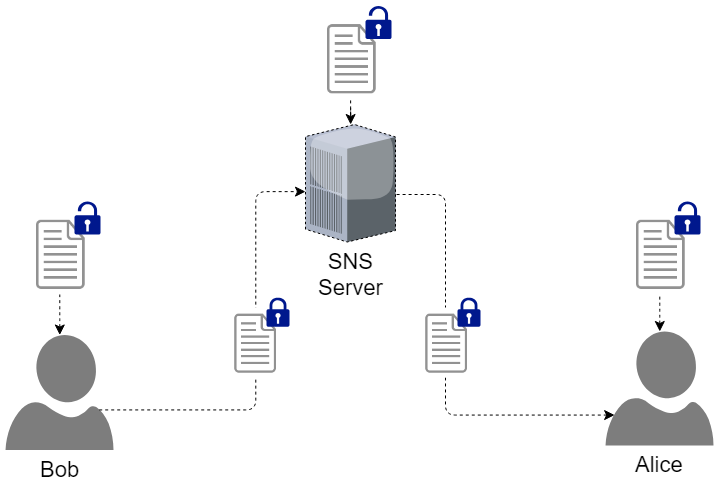
\includegraphics[width=\textwidth]{Figures/SNS}
  \decoRule
  \caption[SNS: False E2E encryption]{False end-to-end encryption used in some SNS. The service has access to the keys used to encrypt the data. This allows the service to decrypt the data you send.}
  \label{fig:sns}
\end{figure}

The use of cloud services has exploded in recent times. The situation today is that if the file attachment is too large, it will often be uploaded to a cloud-service instead and a link to said file attached. While this sort of functionality is easy to use, it makes users lose control over their data. The user is giving a company access to the file that was intended only for the receiver. In reality, the user is giving away ownership of the data and longer has control over how long it is stored, how it is stored or who can access it. The user is at the mercy of the service provider. While it is doubtful that these service providers ignore attackers and disregard the privacy of their users, one would be very naive to assume that it cannot be stolen. There are countless examples of such services being successfully attacked or information being leaked on accident. A few examples are:
\begin{itemize}
	\item Celebgate/The Fappening:\\
	Attackers hacked celebrities' iCloud accounts and gained access to large amounts of private pictures, videos and other data \cite{CelebgateTwoMethodological}.
	\item Verizon leak:\\
	A misconfiguration in the cloud storage of telecommunications company Verizon, exposed the personal information of up to 14 million American customers \cite{CloudLeakHow}.
	\item INSCOM leak:\\
	A large amount of critical data belonging to the United States Army Intelligence and Security Command was leaked onto the public Internet \cite{osullivanBlackBoxRed}.
\end{itemize}

There are also a plethora of SNS that support file transfers. Many of these services boast of being E2E-secure and protecting users privacy. Unfortunately, since there is no way for the users to know how each service handles their information, there is no way to know how secure their solutions really are. There is a precedent for being wary of these services though, as some have been revealed to only encrypt data between end nodes and the server, as shown in \Cref{fig:sns}.  One example of this is Skype \cite{greenwaldMicrosoftHandedNSA2013,popaSkypeProvidedBackdoor,ItSafeTransfer}. While other services may not work the same way, the fact of the matter is that anything going through or being stored on their servers, is out of reach for you as an end user. Would it not be better if you could transfer the file directly to the intended receiver and be in full control over where the file is?
%
\section{Contributions}
%
The intended use case for SendIt as a system is when transferring sensitive files. For whatever reason one might have to keep data private and confidential, when transferring such data online, SendIt will be able to provide the necessary service.

One example may be for companies transferring personnel-files between their offices. A lot of companies outsource data storage and management. As such, sending personnel-files, which then get uploaded to a cloud storage, may in fact be illegal, since the company is no longer in full control of the data. This is an unnecessary risk as direct transfer is quicker, easier, and limits liability in these cases. Not only that, but it also removes the need for storing the file somewhere in transit, which removes the risk of it being stolen if an attacker gains access at a later date. We can conclude that in cases such as these, SendIt is an overall improvement compared to the current alternative. The arguments for this example can be used for any transfer of sensitive or private data, and as such is applicable to a variety of scenarios. Thus, the use cases of SendIt are many, but mainly focused around transferring confidential or private data.

Many solutions to share files already exists, with a few mentioned previously (\Cref{sec:related}). The exchange and management of identities combined with peer-to-peer transfer and trust evaluation is original to SendIt. The combination of these technologies into a singular system constitutes my original research activity. 
\paragraph{}
This thesis' contributions can be summarized as follows:
%
\begin{itemize}
	%
	\item Serverless implementation of WebRTC in larger systems:\\
	This thesis goes to show that serverless implementations of WebRTC can be used in larger systems. The thesis evaluates the advantages and disadvantages of such a solution in contrast to more commonly used solutions, both for WebRTC and other technologies. The advantages of not having a server broker all connections are many, and if IPv6 becomes more popular, an increase in such solutions are likely to occur due to the fact that NAT traversal will no longer be necessary. This in turn makes it easier to connect directly to endpoints. It would also allow for companies to provide services while lowering the cost of providing such services since they no longer need to provide servers to broker connections, greatly increasing profit margins. This would be very beneficial, especially for VOIP solutions, which is currently one of WebRTCs main usages.
	%
	\item Client-only development:\\
	A benefit following the serverless approach is that only a client application is necessary to use the service. No centralized program or dedicated servers are required for the service to stay operational. This reduces development time, resources needed, lowers attack surface and results in simpler implementations. Many programs exist only locally, but being able to communicate over the internet using such programs, is rare. Usually at least one connection to a centralized server or node is required for such programs to work. This is not the case for SendIt, and as such, opens up a new venue for application development.
	%
	\item Propose a new system that can be expanded as needed:\\
	A system offering endpoint authentication and direct P2P connections, while still being easy to use, is non-existent in todays technical environment. By introducing such a system, better security becomes available to the masses. It also functions as a platform which one can modify and build on to improve current functionality, or add new ones. It is easily expandable and can be used as a platform for any kind of application over the internet. It lays the groundwork so others can focus on the specifics of their solution, instead of worrying about connection setup or authentication of users.
	%
	\item Direct connections between users:\\
	%
	As mentioned in the \Cref{sec:motivation}, one of the goals of this thesis is to go back to the idea of a decentralized internet. A direct connection, when possible, is a big step in the right direction. By utilizing P2P this is easily achievable. The problem comes down to identification, authentication, and protecting the integrity of the data sent. This is rarely needed, however, as P2P is not commonly used in systems that require any kind of authentication. In such systems, tokens issued by a server can be used as authentication. By creating a system using P2P and avoiding the use of a central server, problems arise. These problems can be solved by combining P2P and public-key cryptography, but this again raises the issue of creating trust and trust management, since this is usually taken care of by the server. By using the web of trust model, this problem can be mitigated. This type of complete system for direct connections is new and original.
	%
	\item New perspective on e-mail attachments:\\
	%
	It is about time this functionality gets a rework and improved implementation. It has been largely unchanged since it was implemented and is in desperate need of being replaced. This thesis suggests a new system that can easily be implemented in both online, as well as local e-mail clients. It can be used as either a supplementary system, or a replacement. To properly replace the current system, some updates and extended functionality would have to be added to the proposed system, but most of the work is already done. To clarify: this thesis is only one of many ways to improve the current system. A combination of solutions will probably yield the best results. What this thesis aims to do is be one of the better, if not the best, currently available solution for those who value usability and security.
	%
	\item Security to the people:\\
	%
	From a layman's perspective, computer security as a discipline is difficult. The computer only became mainstream in the last \textasciitilde25 years, and as such, society has not yet completely adjusted to this new technology, especially the security aspect of it. While most of the workforce has adjusted and can now perform their tasks on a computer, they do not have a deep understanding of how computers work. Most users are not qualified to make judgments about how secure a solution is, or how it should be used. They rely on the IT departments to serve them easy to use applications that are customized for the intended purposes. These people occasionally need access to equally secure solutions as someone with a security background, but do not have the skills to use the same tools as the security professionals. As such, applications abstracting away all the technology and allowing for easy to use, secure systems are needed. This seems largely ignored by the security community today, as most applications are command-line utilities, or have extremely underdeveloped GUIs. SendIt tries to remedy this by being a system that allows users to focus on the task they want to accomplish, file transfer(s), while taking care of the security and technical challenges on behalf of the user.
	%
	\item All of the previous points combined:\\
	All items on this list may not be original, but combined they result in a unique approach to a problem that is largely overlooked. No other system has the combined properties outlined, which makes SendIt the first of its kind. Hopefully, this thesis will contribute to, and put focus on, the issues previously stated and lead the way for improvements and better solutions in the future.
	%
\end{itemize}
%
%
\section{Organization}
%
The thesis is organized as follows:\\
% 
\begin{itemize}
	\item \Cref{Chapter2} explains the technology and principles used in SendIt and gives a thorough review of the background for choosing them.\\
	%
	\item \Cref{Chapter3} goes through the concepts and design of the base system. It reviews the basis for the functionality of SendIt. It also discusses the design of the ACS server.
	%
	\item \Cref{Chapter4} examines the implementation of SendIt, based on the concepts and design discussed in the previous chapter. It shows how the application looks and functions, as well as how the ACS server is implemented. It will also give an overview of the extendability of the system.\\
	%
	\item \Cref{Chapter5} will discuss the design and implementation chosen for the two modes. It will show the use cases for each mode, discuss advantages and drawbacks and indicate how to best take advantage of the given functionality of each mode.\\
	%
	\item \Cref{Chapter6} will discuss the experiments done as part of the research. It will give an overview of the motivation for doing the experiments, the methods used and the impact and findings of the experiments.\\
	%
	\item \Cref{Chapter7} examines and evaluates SendIt as a system and compares it to existing systems. The analysis is focused on the security and usability of these systems.\\
	%
	\item \Cref{Chapter8} concludes the thesis by summarizing the contributions and work done. It also discusses future work and possible improvements.
\end{itemize}

% Chapter 2
%
\chapter{Technology and Basic Principles} % Main chapter title
\label{Chapter2} % For referencing the chapter elsewhere, use \ref{Chapter2} 
%
%2. Technology and basic principles
    %
    %Public Key Cryptography
        
        %Key management

        %Certificates
        %\label{sec:cert} %Discussion of what data certificates usually contain

        %\label{sec:pgp_enc} %Demmonstration/Example of PGP encryption

    %Web of Trust
        %Overview

        %Ceritifcates

        %Certificate sharing

        %Sylbil attack
        %\label{sec:trust_syl} %Sylbil attack theory

    %WebRTC
    %\label{sec:webrtc}
        
        %Connection setuo
            %ICE, STUN \& TURN
            %\label{sec:webrtc_icetri} % WebRTC ICE trickling
            %SDP and DTLS-SCTP
            %Offer and Answer
            %\label{sec:webrtc_off} 

        %Signaling server

    %WS
    %\label{sec:ws}
    
%
% THIS SHOULD GO THROUGH THE TECHNOLOGY OBJECTIVELY AND HOW IT WORKS!
%
This chapter will go over the technologies proposed and used in SendIt and give an introduction to their functionality, as well as the reasons for choosing that technology. It will give a basic understanding of the technology, which the rest of the thesis is built upon.
%
\section{Cryptography}
\label{sec:pkc}
%
    %TODO
    %Key pairs
    The encryption and authentication scheme used in SendIt is based on public key cryptography and symmetric cryptography. Public key cryptography is a technology that creates a public and a private key pair. The public key is used for encryption. The encrypted data can \emph{only be decrypted by the corresponding private key}. The inverse is also true. Anything encrypted with the private key, can be decrypted by the public key. The common usage is to spread the public key around, hence the name public. The private key (also called secret key) is kept safe, and only the identity that is the owner of the key pair should have access to it \cite{trcekManagingInformationSystems2006}.

    In contrast, symmetric cryptography utilizes the same key for encryption and decryption. The advantage of symmetric cryptography is that it can encrypt larger amounts of data. The disadvantage is that anyone with the key, can read any message. Symmetric keys usually also needs a value called IV (\emph{Initialization Vector}), that is used to randomize the encrypted values. It allows for two identical messages to have different ciphers. There are two forms of IV schemes. One is using completely random number(s) each time. This is called a randomized scheme. The other scheme is called stateful, and requires each IV to be unique \cite{bellareIntroductionModernCryptography2005}.

    SendIt uses public key cryptography to exchange encrypted messages that only the person having the correct key can decrypt. This is the same principles as used in Public Key Infrastructure. The difference lies in that PKI relies on a central authority for signing and verifying the keys used, in the form of certificates. SendIt tries to avoid any central form of governance, and as such implements the web of trust model instead, to avoid this central management. This is discussed more in \Cref{sec:trustmodel}.

    \subsection{Key management}
    This means that the keys have to be the same every time, which requires each user to store their keys for later. This should be done with some consideration, since a stolen private key means anyone can now take your identity and successfully authenticate as you. As such the need for secure storage arises. This can be solved by encrypting the keys with a password, then storing them on the local machine. Only when a key is in use, will it be read and decrypted. This decreases the chance of the key being stolen, since it minimizes the attack surface by only having the key available when it is in use.

    When storing keys it is necessary to keep more information than just the key. For example it is also necessary to know who it belongs to. For the proposed system, information relevant to the trust-level of each key also needs to stored. The easiest way to do this, is to store the certificate of each key with the key. That means the trust for a key will have to be re-calculated every time it is loaded. This is costly when it comes to computational resources, but allows the system to re-calculate the trust  in a key before each use. This gives a flexible and up-to-date environment where trust is evaluated similar to in the real world.

    \subsection{Certificates}
    \label{sec:cert}
    %
    SendIt also proposes to use digital certificates, like the ones used in the web of trust model \cite{ar_pgp}. Certificates traditionally contain lots of information. The certificate is then signed by any number of “introducers”, by encrypting it using their private key. An introducer is an identity who trusts another identity and vouches for the legitimacy of that identity \cite{ar_pgp}.
    
    Certificates used in PKI are required to contain enough information to provide a third party with the subject's public key. Usually certificates used in PKI contain more data than required. The minimum require data can be summed up in four points \cite{vaccaPublicKeyInfrastructure2004}:\\
    \begin{itemize}
        \item CA identification information
        \item Subject identification information
        \item Subject public key
        \item Validity (time)
    \end{itemize}
    More information on introducers and certificates can be found in \Cref{sec:trustmodel}.

    \subsection{Authentication}
    \label{sec:pgp_enc}
    The last part of the puzzle is: how can a user be authenticated based on this information? There are many different schemes but SendIt focuses on the one suggested by PGP for securely exchanging messages \cite{b_pgp}. The system is based on public key encryption. It also uses a session key, which is a random, one time generated symmetric key. The system guarantees the authenticity, confidentiality and integrity of the data. Encryption and decryption using the PGP system is shown in \Cref{fig:enc} and \Cref{fig:decr}.

    The way PGP works is by first generating a symmetric key and encrypting the data to be transferred with this symmetric key. This results in a cipher. Let us call this \emph{Cipher 1}. Then the symmetric key is encrypted with the recipients public key. This also results in a cipher. Let us call this \emph{Cipher 2}. The data transferred to the recipient is Cipher 1 and Cipher 2.

    The recipient then retrieves the symmetric key, by decrypting \emph{Cipher 2}, using their private key. Then, using the retrieved symmetric key, \emph{Cipher 1} is decrypted and the original data is available.

    This solution is made with a one-directional exchange of data in mind. We will be using this system to authenticate both endpoints, which means we will have bi-directional communication. The way to solve this issue, is by taking advantage of the way symmetric keys encrypt data. The initial exchange from Sender to Receiver gives proof to the Sender that the recipient is as intended. This is not the case if we re-use the same IV for the reply back. As such, it should be changed.

    Usually the IV is shared in cleartext, since knowledge of the key is required to decrypt it, so it is not sensitive data. In SendIt we encrypt the IV used in the reply with the recipients public key. That means that in order to be able to access the data, the private key is needed, and as such, the Sender is also authenticated. This solves the issues of mutual, bi-directional authentication.

%
\section{Web of trust}
\label{sec:trustmodel}
%
    This section is a suggestion and evaluation of the system only. This has not been implemented in SendIt due to time constraints, but is considered a part of the design.

    \subsection{Overview}
    The model suggested is based on the web of trust model. The web of trust model says that trust should be split in to two groups: \textbf{Trustworthiness of public-key certificate} - \emph{How willing are you to trust this key pair when it is being used to communicate?} and \textbf{Trustworthiness of introducer} - \emph{How willing are you to trust this key pair when it is being used to introduce another key?}.

    It also suggest that the trust level given to a key should be based on points given to a certificate, based on the sum of introducer's and their respective trust level. There is no concrete policy or algorithm suggested for evaluating which level of trust is assigned. The paper does define levels of trust, but they are different for the two groups mentioned above. 

    There is also no recommendation of which trust level should be considered safe or unsafe. This is left up to each individual user \cite{ar_pgp}. There exist many ways to rate and evaluate trust. For this system, a simple point-based system is likely to be the best fit. The web of trust model has also been recommended by other researchers, albeit for a more traditional WebRTC authentication system \cite{ar_whois}. For a look in to more options, J\o sang et al. 2007 \cite{a_trustserv} gives a good overview over possible alternatives.

    \subsection{Certificates}
    %
    The way one infers, evaluates and determines trust is by using certificates. The trust is evaluated based on interactions with others and the interactions between trusted introducers and others. This means that information from identities one does not trust will be disregarded (their introductions mean nothing), while still valuing and receiving updated information from identities one does trust.In other words, many untrusted identities introducing someone does not hold any value, while introductions from a few trusted identities has a significant impact on the trust level assigned to a certificate.

    \subsection{Certificate-sharing}
    The exchange of keys and the trust each identity assigns these keys are central to the web of trust model, as described above (\Cref{sec:trustmodel}). Since the connection used for communication is already secure and each party authenticated, this data can be transferred without additional encryption. This section will describe how this is intended to be implemented in SendIt. This is included as part of this Chapter since it has not been implemented in practice.
    %
        \subsubsection*{Request certificates:}
        SendIt will have an automated, bi-directional sharing of certificates, that happens on every exchange. This sharing will be part of the file transfer-protocol and will happen after the file-transfer has completed (before terminating the connection). This automatic sharing will abstract the system away from the user, to make the system easy to use and understand, while still updating the trust-level for different identities according to recent changes in the system. The choice to make this part mandatory also allows for the system to avoid being biased by only receiving updates from certain identities.
        %
        \subsubsection*{Evaluate certificates:}
        While exchanging certificates with all communication-partners is important to avoid biases, it is also important to let the user influence and differentiate the level of trust given to each partner. This is where settings and evaluation comes in to play. Each user can change the level of trust in each partner manually, based on his own preferences.

        As an extension of the trust given to each partner, the information they share, is also evaluated based on how trusted the partner is. The trust evaluation of each key, and by extension each identity, will vary depending on user settings and preferences. It will however always follow the scheme as described above. The effect of this evaluation will result in a corresponding trust-level associated with the identity. Identities that have too low a trust level to be used can either raise a untrusted-user warning before communication occurs, or a connection terminated message, depending on the users settings. These keys will still be stored in the users key-chain and stay available for future evaluation, even if their current level of trust is low.

    \subsection{Sylbil attack}
    \label{sec:trust_syl}
    A common attack in decentralized reputation systems is the Sybil attack. It is an attack that takes advantage of the fact that the system can be manipulated by having a large number of identities share the same, false information to innocent identities. In SendIts case, that a certain key pair belongs to a certain identity, while in fact it does not. Through sheer numbers, the attack manipulates identities in the system to believe that the attacker should be the trusted identity, not the original identity. This misleads users to connect to the wrong identity, which makes them vulnerable to attacks. It can also lead to being unable to connect to the legitimate identity, since all traffic for that identity is instead routed to the attacker \cite{lncs_sybil}.

%
\section{WebRTC}
\label{sec:webrtc}
%
    WebRTC is a fairly new technology developed for real-time communication between web entities. It focuses on allowing video, audio and data transfers over P2P, through an easy to use API. It does this without the need to install plugins or having to download native applications, since it is already implemented in most of today's popular browsers. 

    %Connection setup
    \subsection{Connection setup}
    \label{sec:conn_setup}
    %
    To set up a connection using WebRTC, there are different variables one has to take in to account. First, what are the network conditions for each endpoint? To be able to create a connection, we need to find a way to address each endpoint directly. To do this WebRTC utilizes STUN \cite{ar_stun} and/or TURN \cite{ar_turn}, and ICE \cite{ar_ice}. 
    %
    \subsubsection*{ICE, STUN \& TURN}
    \label{sec:webrtc_icetri}
    %
    The ICE-protocol works by trying to connect directly to the endpoint. If an endpoint is behind symmetrical NAT, however, a TURN server is required. A TURN-server acts as a relay-server that both endpoints connect to, and there is no longer a direct P2P-connection. Instead each endpoint is connected to a server by a P2P-connection, and the server forwards information to the other end. It is the ICE-protocol that manages these issues and tries to find the best possible connection \cite{ar_webrtc_sign}.

    %Add more detail on ICE trickling! Picture? TODO
    ICE is a protocol for NAT-traversal used in offer/answer protocols. In regular WebRTC-applications, something called ICE-trickling is used. This is because generating the offer and the answer is quick, but gathering ICE candidates takes time. This allows the setup of the channel to happen first, then ICE-candidates to be shared afterwards \cite{ar_ice_trickle}. In SendIt this functionality is utilized in the ACS mode.

    In serverless mode all the information is gathered, then attached to the offer/answer and then shared. ICE is used to be able to address and reach computers behind NAT \cite{ar_ice}. The easiest way to describe the whole process is to imagine ICE as the decision maker, utilizing STUN and TURN to find information about the endpoint. Once all the information from STUN and TURN is gathered, ICE prioritizes the information, and shares it as separate possible ways to connect to the endpoint. These connection alternatives are called ICE candidates.
    %
    \subsubsection*{SDP and DTLS-SCTP}
    %
    SDP stands for Session Description Protocol, and is a format for session descriptions. This is a protocol for formatting data, for example discovered through the ICE-protocol, to be shared with the other endpoint \cite{ar_sdp}. For the serverless mode, it is up to the users how they share the offer and answer, and as such it does not use a transfer-protocol. In the ACS mode, secure WebSockets are used for sharing the information.

    The WebRTC datachannels used for direct communication uses DTLS-SCTP as their transport-protocol \cite{ar_webrtc_dc}.
    %
    \begin{quotation}
        \enquote{DTLS itself is modelled upon the stream-orientated TLS, a protocol which offers full encryption with asymmetric cryptography methods, data authentication, and message authentication \cite{StudyWebRTCSecurity}.}
    \end{quotation}
    %
    In other words, the communication is securely transported between the endpoints, once the connection setup is done.

    %WRITE XEXPLICITLY! TODO
    The encapsulation of SCTP over DTLS, ICE- and SDP-protocols are complex. For those unfamiliar with the technology, an in depth explanation is given in Holmberg, H.-C. (2015)\cite{url_webrtc_data}. In summary: each endpoint gathers the necessary connection data and then formats it according to the SDP-protocol, for session-negotiation and initiation. Then the datachannel is created and the connection is made.
    %
    \subsubsection*{Offer and Answer}
    \label{sec:webrtc_off}
    %
    Following is how the relevant RFC describes how endpoint guarantee is done:
    %
    \begin{quotation}
        \enquote{A certificate fingerprint is a secure one-way hash of the DER (distinguished encoding rules) form of the certificate. If the X.509 certificate presented for the TLS connection matches the fingerprint presented in the SDP, the endpoint can be confident that the author of the SDP is indeed the initiator of the connection \cite{ar_tls_sdp}.}
    \end{quotation}
    %
    This explanation can be a little hard to understand, so let us break it down. Both the offer and the answer generated by the WebRTC API has a fingerprint of a certificate attached. The endpoint generates a X.509 certificate and a corresponding private key. By matching the fingerprint received during signaling, with the certificate used during the setup of the DTLS-SCTP connection, one can be certain that the endpoint is the same. This is illustrated in \Cref{fig:DTLS_setup}.
    %
    \begin{figure}[t]
      \centering
      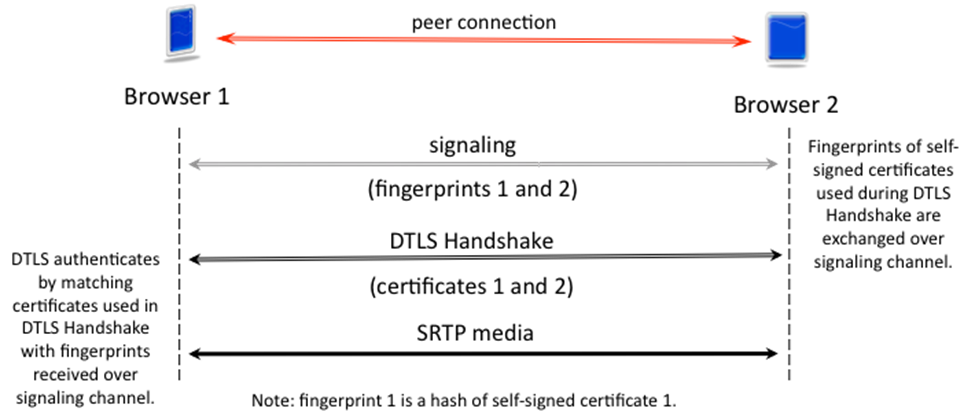
\includegraphics[width=\textwidth]{Figures/DTLS_Exchange}
      \decoRule
      \caption[DTLS setup]{Illustration shows and describes how DTLS is setup between two endpoints. The final channel in the illustration is of the type SRTP, but the same procedure is true for SCTP \cite{WebRTCManMiddle2015}}
      \label{fig:DTLS_setup}
    \end{figure}
    %
    \subsection{Signaling server}
    \label{sec:sign_serv}
    %
    In the usual use-case of WebRTC, a signaling-server is used to share SDP offers and answers, as well as continuously sharing ICE-candidates. This separate channel allows for re-negotiation of communication, if the connection breaks down. An offer is the exchange of SDP information from the sender, to the receiver. An answer is the exchange of SDP information from the receiver, to the sender.

    There is several reasons for the usage of a signaling-server. One is the ability to reconnect in the event of a failure in the established connection. Another is that it allows the offer and answer to not be created until both endpoints are online, then immediately created and shared. This is the case when using ACS. When using serverless mode, however, this is not the case. This means it is affected by the fact that network conditions can change rapidly and as such ICE-candidates may no longer be viable, leaving endpoints with no way to make a connection or renegotiating the connection. For more information on the lifetime of the exchange, see \Cref{Chapter5}.

    Another use of the signaling-server is that it allows for encrypted communication between the parties, via the server. As long as you trust the signaling-server, your communication is confidential. This is important in regards to the exchange of the offer/answer, as they contain information that allows a secure connection to be set up, as described in the section above.

    In the Serverless mode we do not have a secure channel over which we exchange the offer/answer. That means it would be vulnerable to a MitM-attack. To combat this the offer and answer will be encrypted by each endpoints public key, on all connections after the first (See \Cref{fig:enc} for illustration). With this protection in place an attacker can not get a hold of the offer/answer, without stealing the private key that can decrypt the cipher.

%
\section{WebSockets}
\label{sec:ws}
%
To understand why WebSockets are necessary, let us first examine how normal communication between client and server is done. The client sends a request and the server sends a response. If the data contained in the response is time critical, it will in many cases already be outdated by the time it is rendered by the client. A manual way to combat this is to refresh the page. A more elegant way is the use of polling. Polling is a regularly timed, synchronous call the client makes to the server, to look for new information. This works well if you can predict when new data will be available. The problem is that this is often not the case. There are other alternatives as well, for example long polling or streaming, but they all come with certain issues regarding real-time, two-way communication. Especially latency and overhead are big issues.

This is where WebSockets come in to play. WebSockets offer real-time, duplex, bi-directional connection. It makes communication between a client and server easier and faster. It also supports real-time communication, which is an added bonus. WebSockets are commonly used in a lot of real-time applications in today's online environment. From transferring game data to simple chat applications. It is also commonly used for signaling in WebRTC applications. This is also how it is used in SendIt, specifically in the ACS mode.

Another great thing about WebSockets, is that it supports the traditional use of TLS. This means that the WebSocket protocol can use the same security mechanisms as traditional HTTPS traffic. This makes it easy to protect the confidentiality, integrity, and availability of your network communications. Finally, all modern browsers have native support for the WebSocket protocol and as such it is incredibly easy to deploy \cite{wangDefinitiveGuideHTML52013}. For these reasons, the WebSocket protocol was chosen to take care of the communication between endpoints and the Server, required by the ACS mode.


% Chapter 3
%
\chapter{Concept and Design of SendIt} % Main chapter title
%
	%Concepts
		%First trust
		%Trust building & factors (timing etc)
		%Authentication
			


\label{Chapter3} % For referencing the chapter elsewhere, use \ref{Chapter1} 
%
This chapter will discuss the overall concepts and design of SendIt. It will illustrate how SendIt utilizes the solutions discussed in \Cref{Chapter2} and how this is beneficial to the system as a whole. In addition, general information relevant to the application and system will be discussed here. It will also discuss the design of the ACS server.

%
\section{Concepts}
%Concepts
%
The following concepts and assumptions build the base of how the technology is applied, while also being a product of the technological limitations and how this technology is implemented. The concepts introduced are a mix of new concepts and ideas and concepts borrowed from previous research. The assumptions are a result, and consequence, of the initial idea of the system, as well as the technological limitations imposed by the chosen technologies, combined with the lack of better options. These assumptions were necessary to narrow down the work and to be able to keep the system simple for the end users. While these assumptions may limit or reduce some of the security measures available, the limitations they would impose on the usability were considered more important.

%
	\subsection{First trust}
		%
		The first trust, or initial trust, is the basis of every interaction in every computer system, as well as in the real world. In the real world, you can see the other person, and as such, easily identify who it is. This is not the case in computer systems, therefore, a way to identify entities is necessary. In this system, the choice was made to use e-mail addresses as a basis for uniquely identifying each entity. Since one of the main goals is to improve e-mail attachments, it felt like a natural choice, as well as being easy to implement. Since there is now a way to address each entity, the necessity for confirming that identity arises. This process is called authentication, and how it is done will be discussed more in-depth later.

		To be able to authenticate an identity, the fact that the identity has to possess something unique has to be addressed. If not, someone else can impersonate them. In the real world, everyone has a unique (or close to unique) appearance, which is almost impossible to fake. This is not the case for computers. Usually the PKI model (explained in \Cref{sec:pkc}), is used to vouch for the validity of an identity in computer systems. As explained previously, this requires a lot of setup and cannot be done easily. Because of this, it is not fit to be used in combination with SendIt. 

		SendIt is built on the idea of trusting the first interaction, based on non-absolute authentication methods. This means the first Answer and Offer exchange (connection setup) is done assuming the other endpoint is not malicious. It is done in an unencrypted manner, without any guarantee of the integrity of the message or using any authentication mechanisms. The reason for choosing this solution is that it allows for an easy and convenient way to start communicating with new partners. It is important that the system is kept simple, to keep it user friendly.

		It also allows for an intuitive approach to the first interaction. Instead of having someone's pre-shared secret or other means of authentication, the timing and files shared can be a means of authentication. It feels unnatural to have someone randomly send files to you, unless it is somewhat expected. It is also strange to receive files where the content seems unknown or strange, without any previous communication or knowledge. As such, the argument can be made that this system is more intuitive than the alternatives.

		While the timing and files shared do continue to count towards the trustworthiness of an identity, it is important to note that \emph{only the first interaction is inherently trusted}. All subsequent communication is end-to-end encrypted and the endpoint is \emph{always authenticated} before communication starts. As such, if the user takes care to be certain of the endpoints identity for the first interaction, all subsequent interactions are guaranteed to be with the same identity, barring that user having their credentials stolen.

		The take away from this is, while the timing and files shared should still be considered, all subsequent interactions are, by and large, guaranteed to be with the same identity. As such users are encouraged to take extra care during the initial setup, but can relax and trust the endpoint during all future interactions and rely on the system to warn them if something is amiss.

		To sum it up by using a comparative example: If someone were to place a random package outside your door at a random time, with no information on it, one would naturally be wary of the contents and motives of that person. In contrast, if a friend made an appointment to deliver a package that day, one would be much less suspicions, even if it was identical to the package described in the previous scenario. There is no guarantee that the package is from your friend, but it is likely.

		This is the basis of the first trust in SendIt, and allows for an unauthenticated interaction to be the basis of the trust building.  The added benefit is that unlike in the real world, SendIt can guarantee that the package is unaltered and from your friend for \emph{every interaction after the first one}, no matter when it is delivered and what the package may look like.

		There is no denying that this decision leaves the system and end user open to be attacked during this first interaction. The advantage is that it keeps the system easy to use, and allows for a relatively secure system, which relies on human and intuitive factors for establishing the first trust. It relies on machine made, absolute authentication from that point on.

	%
	\subsection{Trust building}
		%
		Trust building in the suggested system, is based on several factors. Before getting into the specifics, it is necessary to point out that the trust system is only a theoretical approach and has not been implemented in the prototype. The proposed system uses trust transitivity \cite{lcns_semantic} (\emph{Trusting in Alice and Alice trusting Bob, means that we trust Bob more, than if Alice was not involved}).

		Other means of building trust includes frequency of communication and bi-directional communication (Acting as both sender and receiver with the same identities involved). Trust built by such activities will gradually accumulate, in contrast to transitive trust. Transitive trust is just a way of assigning an identity a trust level based on the introducers of that identity, and their respective level of trust in said identity. (\emph{How many trusted identities signed, how much do we trust those identities and how much do they trust the certificate?})

		Trust can also be reduced. One event that can cause this is if a user tries to communicate with a previous partner, but that partner is not authenticated according to the key associated with that partner. SendIt's trust system works in a way that gives more weight to reduction in trust. This means it will be harder to gain trust, than to lose it. This is because it is generally a safer approach to be wary, than to assume good faith. In other words, a negative incident will reduce the trust significantly more than a positive incident will increase it. This will help maintain a balanced system that detects untrusted behavior rapidly and acts accordingly.

		%\paragraph{}
		Trust is shared by using certificates. Unlike regular certificates (see \Cref{sec:cert}), SendIt proposes a minimal and simple solution. It proposes that a certificate is just a list of identities and the corresponding cipher. The cipher is made by encrypting the public key of the identity being vouched for, with the users own private key. This way all that is needed to verify the authenticity of a key, is to find the introducer's public key and decrypt the cipher. As such, certificates will contain these fields: Introducer's name, Cipher, and Trust. The cipher is as just described. The trust field is a value of either 1 or 2, where 1 indicates full trust and 2 indicates partial trust. The trust value is included so it is possible to assess how much trust the introducer has in the introduced key.
		%
		\begin{figure}
		  \centering
		  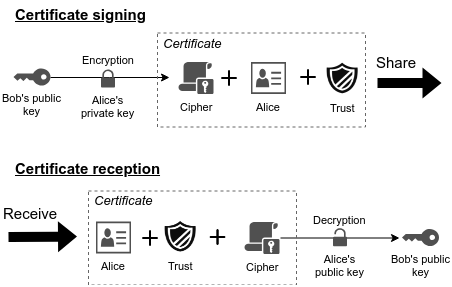
\includegraphics[width=85mm]{Certificate_explained}\\
		  \vspace{1cm}
		  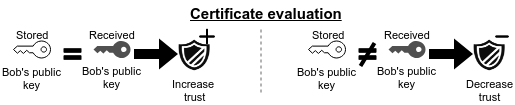
\includegraphics[width=85mm]{Certificate_eval}
		  \centering
		  \decoRule
		  \caption[Certificate transfer and evaluation]{Certificate operations example where Alice signs Bob's certificate.}
		  \label{fig:cert_ex}
		\end{figure}
		%

		When it comes to transitive trust, the specific values and model for assigning trust is not specified, but the idea is to assign different levels of trust, based on the amount of introducers from different trust levels. The level of trust a user has in the introducer of a certificate, directly affects the trust level given to the certificate.

		Once an endpoint has received the certificates, they will be evaluated based on the signatures attached and potentially existing trust values. When the value has been calculated and the new trust level assigned, the key is available like any other and will be used in communications with that identity. See \Cref{fig:cert_ex} for an example. Do note that one certificate can hold many signatures.

		%\paragraph{}
		The practical evaluation scheme for the system is not implemented in SendIt, but the initial idea was to assign these trust-levels based on a point system, where an identity accumulates points by getting verified by introducers that the user trusts. An option is to have different levels of trust, where an identity is assigned a trust level according to the amount of points it has accumulated.

		The amount of points granted for each introducer depends on the trust level the user assigns to the introducer. It also depends on how much this introducer trusts in the key. This is so the nuance of transitive trust is clearer, since the system is based on these nuances of trust. SendIt should have an easy and intuitive trust evaluation, while also having a simple way to fairly assert the trust level of an identity. Unlike the web of trust model, different levels of trust for communication and for introducing keys should not be applied. There should only be one trust level assigned to each identity and it should apply to both uses equally.

		The practical impact of the different trust levels should be visible to the user as a warning, if the receiver does not have a trust level that is sufficient according to the users settings. The user should be able to choose if he wants to ignore the warning or cancel the transfer. If the receiver meets the requirements, no notifications or warnings should appear.

		SendIt should come with pre-configured values so novice users can rely on the standard settings. If they want to change these settings, they should have the option to choose to do so. The users should have an overview of all identities and should also have an overview of the respective trust-levels available in the settings menu, and the option to manually change these levels. This allows the users to override the system in cases where they deem themselves better equipped to evaluate the trust-level of the identity.

		%\paragraph{}
		As noted in \Cref{sec:trust_syb}, the Sybil attack is a problem in decentralized, reputation based networks. The proposed system will not be completely immune to such attacks, but instead look towards making it hard to propagate and become regarded as trustworthy by the majority of identities. This will be achieved by requiring interactions with other identities, as well as a signed certificate from trusted introducers, to gain a high level of trust. By requiring these, in combination, an attacker can not simply create a large sub-network of controlled identities that all trust each other, and then spread it to the main network with the same level of trust.

		This allows for high resistance against this attack, since the attack exploits the fact that a large number of untrusted identities can manipulate how the main network regards the attacker. Since none of these identities will have a high amount of trust in the main network, they will not be regarded as safe. This is true even if they have a large amount of introducers, because the introducers are untrusted identities as well.

	%
	\subsection{Authentication}
		%Authentication

		The authentication scheme in SendIt is based on public-key cryptography. Each identity, or e-mail address if you will, is associated with a unique public and private key. These key pairs are used for authentication. In practice, this is done by encrypting the Offer and the Answer used to establish the WebRTC connection with the other endpoint's public key. This way the ability to connect to each other also acts as authentication, since only the identity with the correct private key can access the information. This explanation is a slight simplification and will be discussed in detail in \Cref{sec:crypto_des}.

		This is in contrast to usual solutions, where authentication is done before initiating a connection. SendIt's solution removes the extra step, and combines these two processes into one. The reason this is made possible is because of how WebRTC's connection setup is done. Because of the authentication built into the Offer and Answer exchange, the system guarantees authentication of both endpoints. For more details on WebRTC's built in authentication of endpoints, see \Cref{sec:conn_setup}.

		As recently noted, the authentication in SendIt relies on key pairs. The key associated with an identity is shared during the first interaction. While there is no authentication of the respective identities during this interaction, the keys are shared over the P2P channel. This channel is end-to-end encrypted, as to not be vulnerable to attacks that manipulate the data in transit. In summary, as long as you connect to the correct endpoint in your first interaction, there is no reasonable way an attacker can impersonate that endpoint at a later time.

		It is also important to note that while the proposed system suggests using e-mail addresses as identifiers, there is no direct connection between the identities in the system and the actual e-mail system. By using e-mail addresses, it makes it easier to add extra trust, by implementing an e-mail verification step if desired. The consequence of this initial separation does mean that the e-mail system has no direct influence or inherent effect on SendIt, but their close relation makes it easy to link the two. This gives all the benefit of the e-mail system, while not having to consider the risks or threats that are inherent to that system. It is left up to the developers and users of SendIt to decide if they believe such a link is a positive or negative addition, and as such their choice to make.
%
%Des
\section{System design}
%SendIt implementation
%
The following section will address the design of the general solutions used in SendIt. It will explore the functionality that is used for both modes, and explain how they work and why they are necessary. It will also build the basis for understanding how the two modes operate, and which functions they build upon in order to work.

	%
	\subsection{Cryptography}
	\label{sec:crypto_des}
%
	\begin{figure}[th]
	  \centering
	  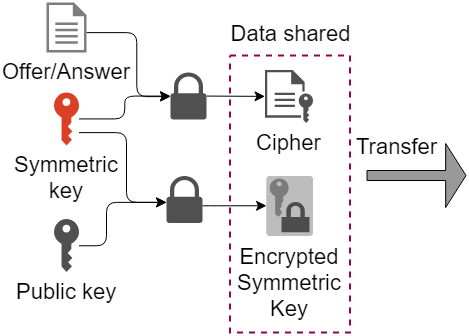
\includegraphics[width=100mm]{Figures/Encrypt}
	  \decoRule
	  \caption[Authentication exchange: Encryption]{In this figure it is shown how the Offer/Answer is encrypted with a symmetric key, creating a cipher. This symmetric key is then encrypted with the recipients public key. The cipher and the encrypted key are then shared.}
	  \label{fig:enc}
	\end{figure}
	\begin{figure}[th]
	  \centering
	  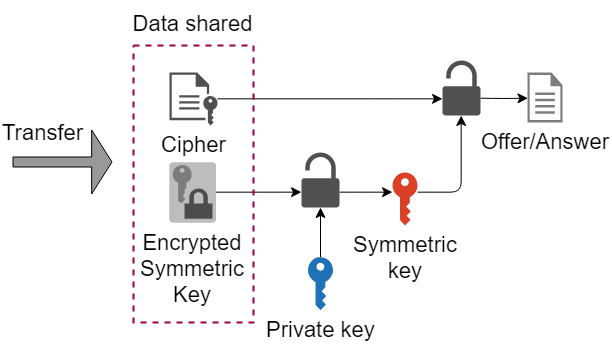
\includegraphics[width=100mm]{Figures/Decrypt}
	  \decoRule
	  \caption[Authentication exchange: Decryption]{Here one can see the received data and how it is decrypted back into the original Offer/Answer. Only the identity with the correct private key can access the original data.}
	  \label{fig:decr}
	\end{figure}

	When a new key pair is created it is not stored on the disk until the public key has been successfully exchanged with another identity, in order to avoid storing unnecessary keys. The file where the keys are stored should be password protected, or otherwise encrypted, to ensure that if it is stolen, it takes considerable effort to steal the keys.

	SendIt also utilizes symmetric keys for encrypting data. These symmetric keys are generated for every session, and used for one session only. The reason symmetric keys are necessary, is because the amount of data that can be encrypted with public-key cryptography is fairly small, and as such, a solution which can encrypt more data is needed.

	The biggest difference between the symmetric keys and the asymmetric key pairs in SendIt, is that the symmetric keys are not stored across multiple sessions. The asymmetric keys however, are stored and stay the same. This is because they are used for authenticating the identities. The way this is done is in a similar fashion to standard PGP encryption and decryption, as explained in \Cref{sec:pgp_enc}. See \Cref{fig:enc} and \Cref{fig:decr} for illustrations on, respectively, encryption and decryption.

	The plaintext in this case is the Offer or the Answer. If it is encrypted, it also contains the encrypted symmetric key, as well as the initialization vector for that key. The initialization vector consists of random integers. The IV is needed to correctly decrypt the data. 

	The difference between SendIt and PGP is that in order to authenticate the Sender, the Recipient needs to encrypt the IV with the Sender's public key and transfer this. If a connection is made, it means both endpoints had to have the correct keys. This is because of the way the connection setup works, as described in \Cref{sec:webrtc_off}.

	\subsection{Protocol}
	%FT protocol
		%How? Which fields? Additions?
	The base protocol used in SendIt is based on the one used in PubShare, an online WebRTC P2P file transfer solution \cite{url_pubshare}. This protocol has been extended and altered to fit with SendIt's needs. This protocol takes care of communicating the status of the file transfer, chunking the data, sharing file metadata, and verification of transfer completion. The protocol is also in charge of setting up authentication of the endpoints, since the data to authenticate eachother should be exchanged directly. This protocol is very limited, and as such, unlikely to have a large overhead and impact on performance, however, this is only an assumption. Following will be a description of the different functionalities of the protocol.

	\subsubsection*{Authentication setup}
	The authentication setup functionality consists of an Authentication setup packet and an Authentication setup reply packet. Both of these packets contain the identity and their associated public key. If one of these packets are received, the system checks that the information supplied does not conflict with existing data. If it does not, and the packet was of the type Authentication setup, the endpoint creates an Authentication setup reply packet and sends it back. If it was of the type Authentication setup reply, the transfer is initiated.

	\subsubsection*{Offer and Answer}
	The Offer packet contains metadata about the files to be sent, so the recipient knows how many files will be transferred, what type of files they are, and how big they are. The Answer packet is just a confirmation that this data was received and that the recipient is getting ready for the transfer.

	\subsubsection*{Request and Data}
	Once the recipient is ready to receive the first data, a Request packet is sent indicating which chunks it wants to receive. It is also used to confirm which packets it has previously received, and to request more data once all the previous chunks have been received. The Data packet contains information about which chunk is being sent, and the file-data for that chunk - the part of the file currently being transferred.

	Following is an example to illustrate how it works: The recipient sends a Request packet requesting chunks 10 through 20. This also confirms all chunks up until 10 is complete. The Sender then transfers these chunks to the Recipient. Once all chunks are received, it requests more chunks until all chunks have been received. If a chunk is not received, the chunk before is treated as the last chunk received, and the chunks afterwards are re-transmitted.

	\subsubsection*{Done}
	The Done packet contains no data field, and is a confirmation that the Recipient has received the file currently being transferred. If there are no more files to transfer, this indicates the end of the connection. If more files are waiting, transfer of the next file will begin once this packet is received.

	\subsubsection*{Cancel and Error}
	The Cancel packet is sent if the user for some reason decides to cancel the current transfer. This interrupts the transfer and closes the connection. If the Error packet is sent, it means an error occurred and the transfer is stopped and the connection closed.

	\subsubsection*{Request metadata}
	The Request metadata packet is only used in the ACS mode. It is necessary so the Recipient can request data about which files are being offered by the Sender, before accepting the connection. 

	%
	\subsection{File transfer functionality}
	%File transfer
		%
		\begin{figure}[th]
		  \centering
		  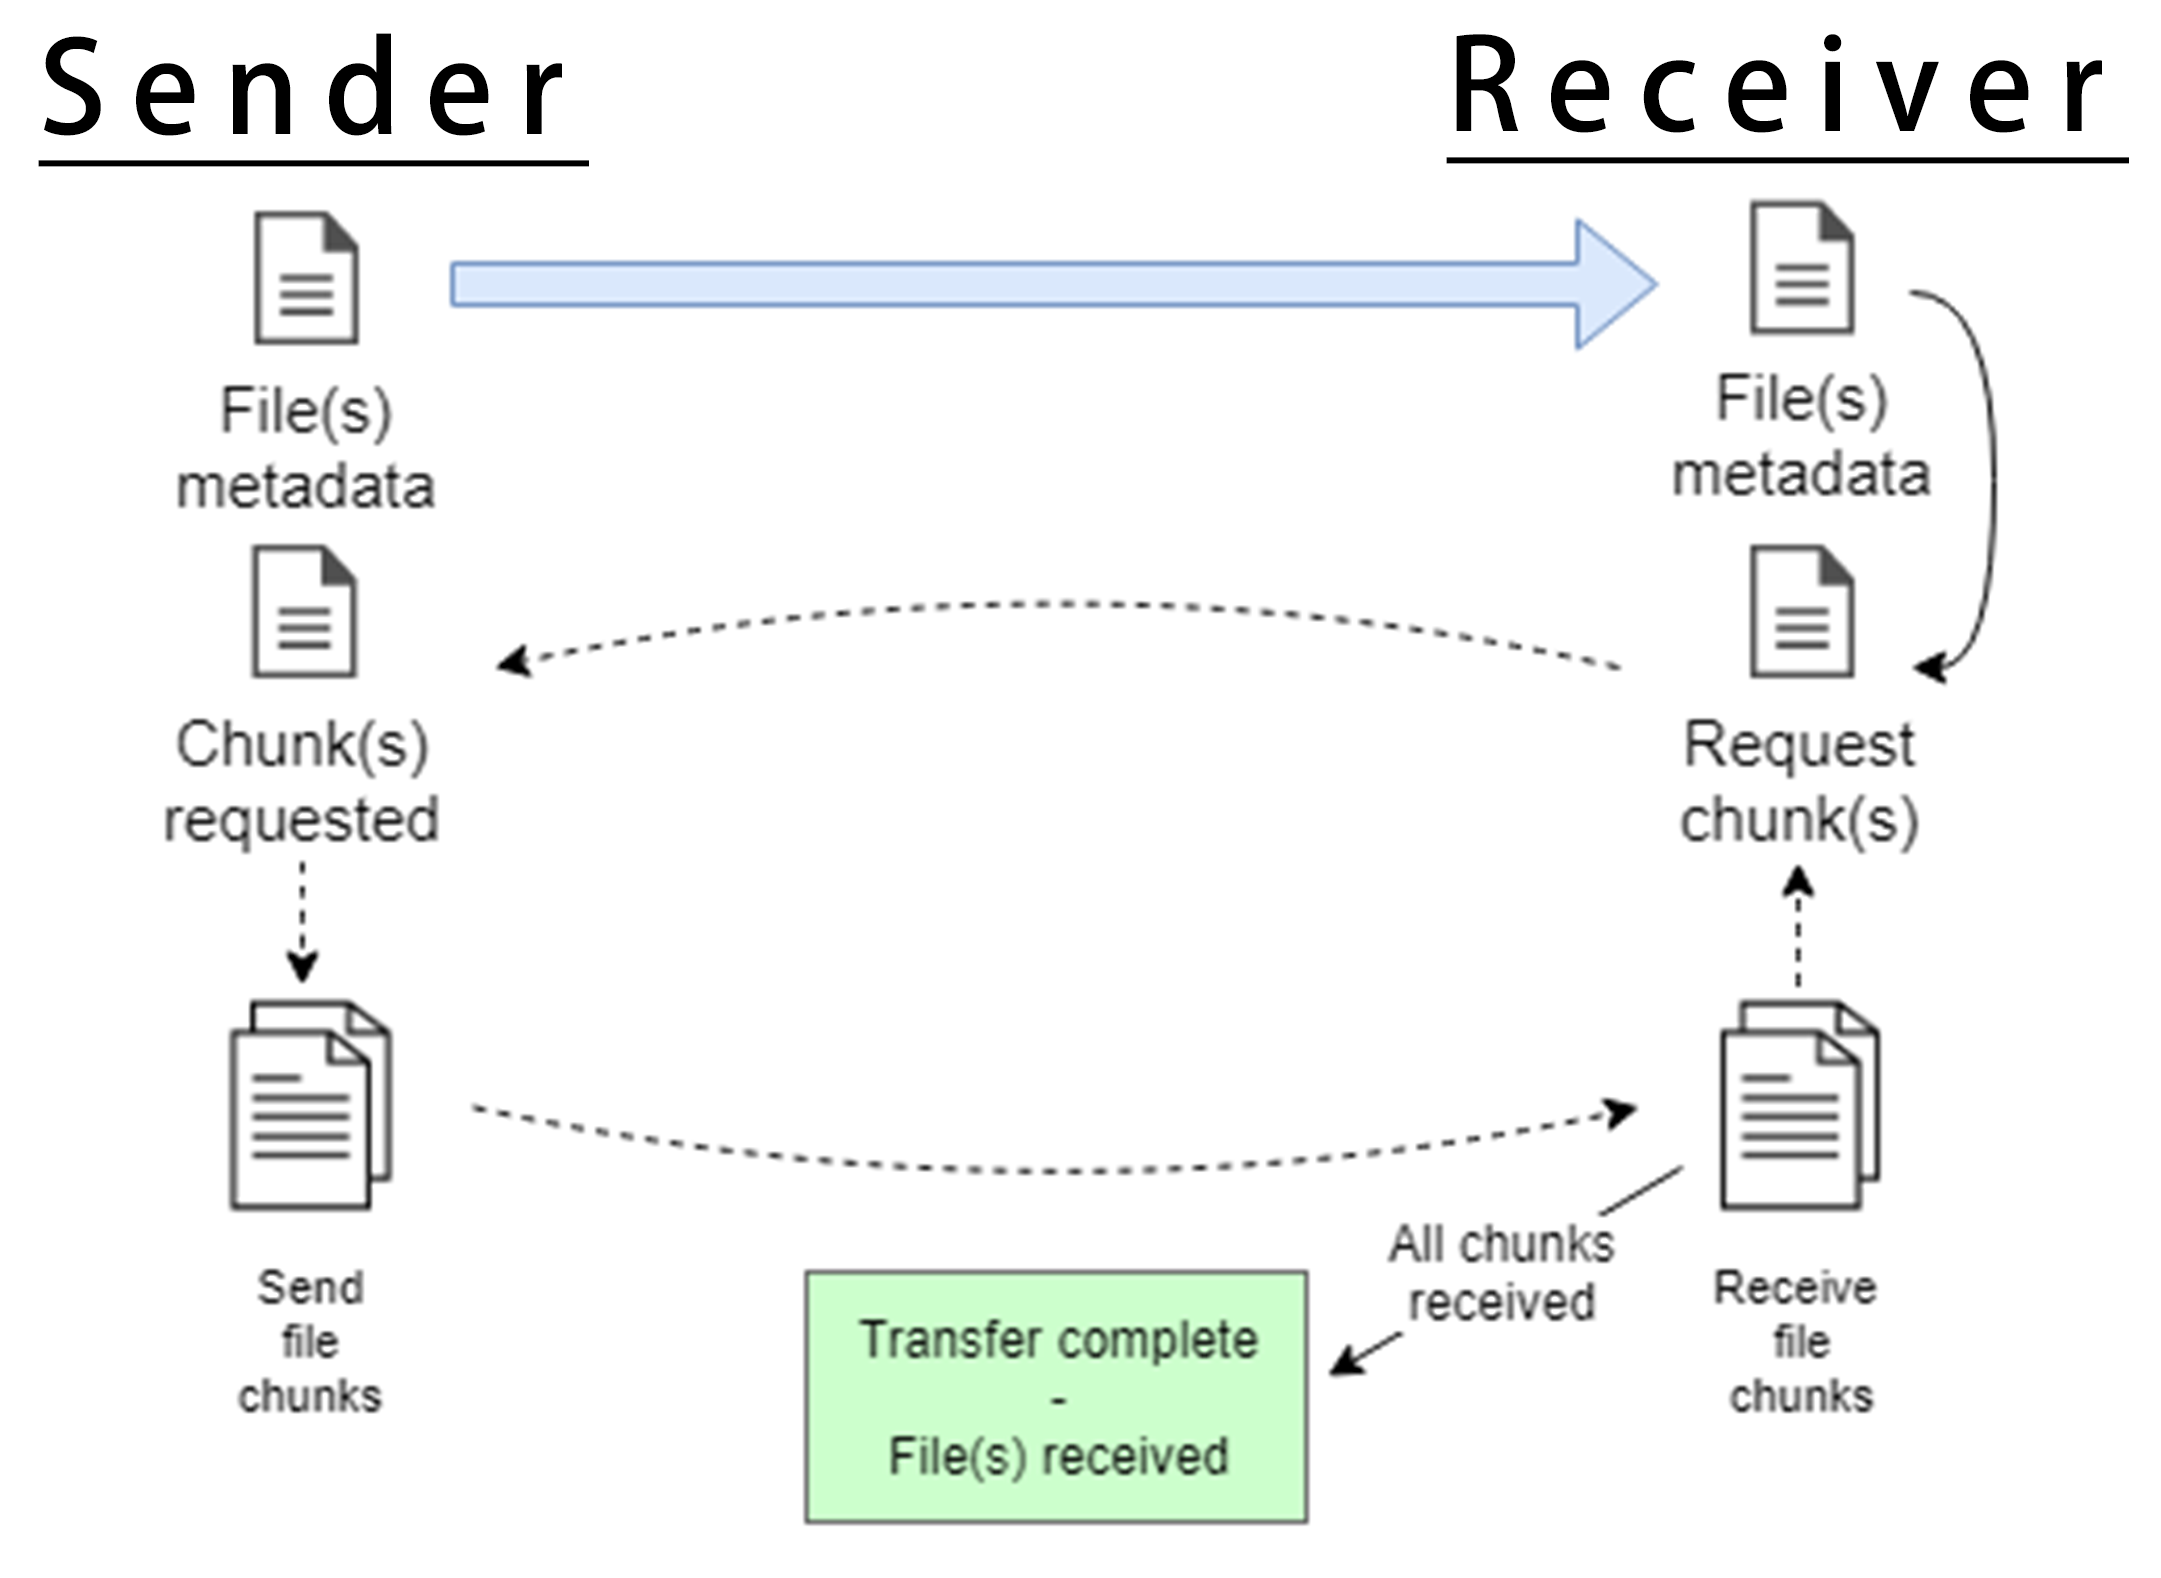
\includegraphics[width=100mm]{Figures/File_share_protocol}
		  \decoRule
		  \caption[File sharing process]{This illustrates the process of transferring file(s).}
		  \label{fig:file_off}
		\end{figure}

		The file is always transferred over a secure P2P channel and with end-to-end encryption. It is transferred using the protocol mentioned in the previous section, in order to manage the transfer.

		Implementing support for bigger files, which means additional chunking, should be relatively easy. As a result, transport of data larger than the current limitations, was not implemented. If this becomes necessary in the future, it can be added as an extra feature. For more on this subject, see \Cref{sec:bigfile}
		
		%File manager
		The chunking, as well as managing which files are to be sent and which files have been received, is done by the File Manager. The File Manager reads a file into memory, then separates the data into chunks. These chunks are then sent through the P2P channel. Once the recipient has received all the chunks, indicated by the metadata previously received, the transfer of that file is regarded as complete. This triggers the chunks to be combined into the original file, and then stored on the recipients computer. It also notifies the sender to start transfer of the next file, or that the transfer is complete.

	\subsection{Modes}
	%
		SendIt operates with two unique modes. One is the ACS mode, which acts as a helper in establishing the P2P connection. The other mode is the Serverless mode, which leaves it in the hands of the end user. What is important to note is that these modes can be selected as the user sees fit. It will also retain information used and gathered in one mode, and utilize it for future connections in the other mode. What it cannot do is transfer data from one endpoint in one mode, to another endpoint in a different mode. Both endpoints have to be in the same mode in order to be able to establish a connection. However, they can switch modes and still connect at a later time, as long as they both utilize the same mode. These modes will be further discussed in \Cref{Chapter5}.

\section{ACS server design}
	\label{sec:acs_serv_des}
	%ACS Server
	%
	The ACS server is in charge of forwarding information from one endpoint to another. It also has some other functionality, like authenticating identities, for the sake of forwarding information to the correct endpoint. The functionality of this server is kept minimal and, as such, should be easy to utilize. It is also easily extendable and deployable, which makes it easy for users to host their own, for their own needs, if they for any reason do not trust any available service.
%
	\subsection{Authentication}
	\label{sec:wsprot_auth}
	%Authentication
		%How? Setup? Usage?
		%
		\begin{figure}[th]
		  \centering
		  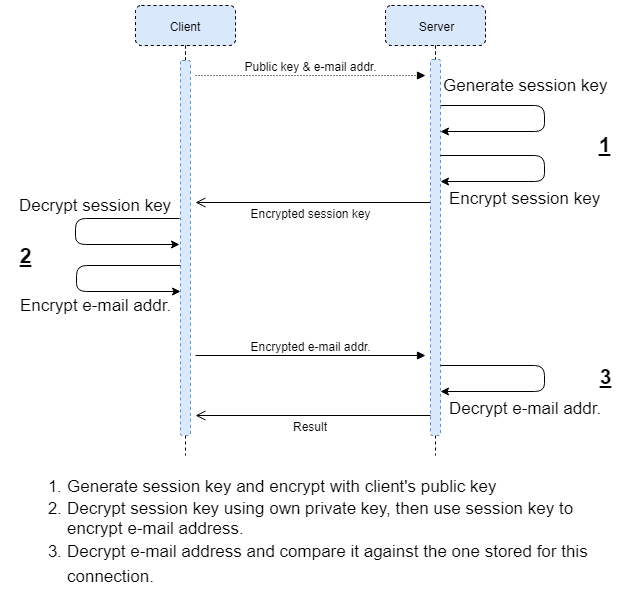
\includegraphics[width=\textwidth]{Figures/ACS_Prot/ACS_server_auth}
		  \decoRule
		  \caption[ACS server authentication scheme]{This figure illustrates how the ACS server authenticates clients. The initial transfer from client to server only happens if they are communicating for the first time.}
		  \label{fig:ACS_serv_auth}
		\end{figure}
		%
		The authentication scheme for the ACS server is extremely simple and just meant as an example for more sophisticated solutions. It works by having the ACS server create a symmetric key and encrypt it using the endpoint's public key. To prove to the server that the endpoint could decrypt the session key, it encrypts it's own identity (e-mail) using the symmetric key and sends it back. If the identity matches the one stored, then the endpoint is authenticated.

		If it is the first time an endpoint connects to the server, the endpoint shares their public key and identity with the server. The server then generates a symmetric key, encrypts it with the public key supplied, and shares it with the endpoint. The authentication scheme is illustrated in \Cref{fig:ACS_serv_auth}.
		
		The reason for incorporating this into the server is that forwarding data to the wrong endpoint could potentially reveal information not meant for that identity. As such, some basic form of authentication should be added to ensure that the information ends up at the right identity. This authentication does not replace or interfere with the regular authentication between endpoints in any way. It is simply a feature added to make sure the data arrives at the intended endpoint.
	%
	\subsection{Communication}
	%
	No code needs to be sent from the ACS server to the endpoint in order to communicate, since all the code is pre-programmed into the client software. As such, the server cannot manipulate nor control the clients behavior in any way, except that intended by the protocol. In this section, when WebRTC is specified, it can be substituted with any Offer/Answer based model or protocol.

	\subsection{ACS Protocol}
	\label{sec:wsprot}
	%
	\begin{figure}[th]
	  \centering
	  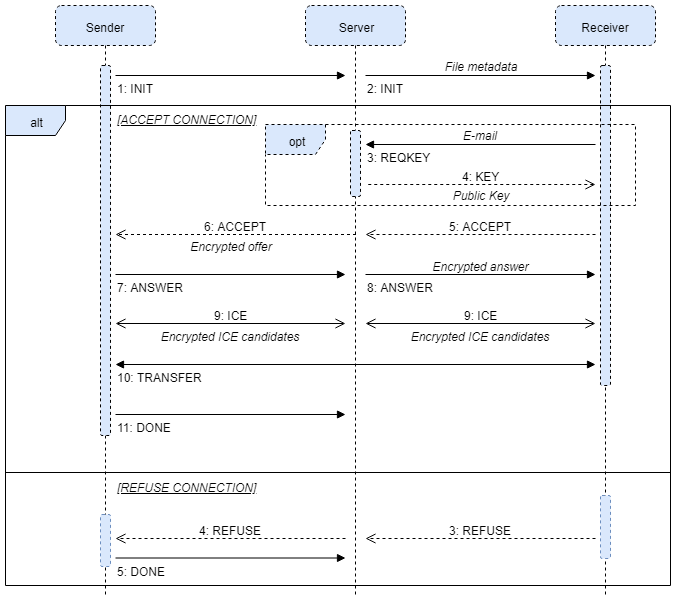
\includegraphics[width=\textwidth]{Figures/ACS_Prot/Communication}
	  \decoRule
	  \caption[ACS protocol: Communication]{This is the main functionality and flow when using ACS mode to transfer files. Do note that the area marked OPT is not implemented.}
	  \label{fig:prot_comm}
	\end{figure}

	%
	The protocol used to negotiate and broker a connection in the ACS mode is made specifically for use with Offer/Answer based protocols. It is kept as minimal as possible, with some of the functionality not yet implemented. This functionality is not necessary, but would improve the system. The basic format of every interaction is shown in \Cref{tab:basic}.

	For an overview of the general communication flow, once authenticated and properly connected, see \Cref{fig:prot_comm}. This is where the main functionality of the ACS server is shown. For information about the specific implementation of this protocol see \Cref{sec:prot_imp}.
	%
	\begin{table}
		\caption[ACS protocol: Basic format]{Basic protocol format}
		\label{tab:basic}
		\centering
		\begin{tabular}{l l l l}
	        \toprule
			\tabhead{Field Name} & \tabhead{Type} & \tabhead{Description} & \tabhead{Required} \\
			\midrule
			Function & String & Name of function & Yes\\
	        Origin & String & E-mail address & Yes\\
	        Destination & String & E-mail address & No\\
	        Data & JS Object & Relevant data & No\\
			\bottomrule\\
		\end{tabular}
	\end{table}
	%
	\paragraph{}
	%
	\begin{figure}[th]
	  \centering
	  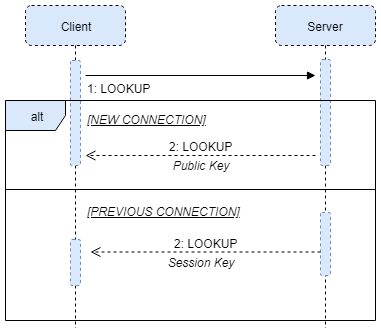
\includegraphics[width=80mm]{Figures/ACS_Prot/Connect}
	  \decoRule
	  \caption[ACS protocol: Lookup]{The lookup function exists so that the endpoint knows whether to start an authentication setup or an authentication process with the server.}
	  \label{fig:prot_lookup}
	\end{figure}

	\subsubsection*{Lookup}
	%SMALL PART IS IMP!
	The first interaction between the client and the server is the \emph{lookup} packet. The client connects to the server, and sends a \emph{lookup} packet containing the identity's e-mail address. If the server has previously communicated with the identity, it will create and send a session key (symmetric key) encrypted using the key associated with the identity. If it has not previously communicated with the identity, the servers public key is sent.

	The flow of this procedure is shown in \Cref{fig:prot_lookup}. This functionality is necessary so the endpoint knows if it should initiate an authentication setup (if there is no associated key in the server) or an authentication process (if there is an associated key in the server).

	%
	\begin{figure}[th]
	  \centering
	  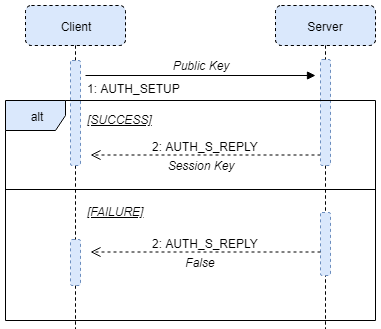
\includegraphics[width=80mm]{Figures/ACS_Prot/Auth_Setup}
	  \decoRule
	  \caption[ACS protocol: Authentication setup]{This shows how the authentication setup happens, and the data which is exchanged between the server and client in the two scenarios. The setup fails if the ACS server already has information stored for the given key or e-mail address.}
	  \label{fig:prot_setup}
	\end{figure}	

	\subsubsection*{Authentication setup}
	The authentication setup between a client and the ACS server is illustrated in \Cref{fig:prot_setup}. This happens the first time an identity communicates with an ACS server and allows the ACS server to be sure that it is always communicating with the same endpoint for any given identity. The endpoint sends it's public key, attached to an \emph{Authentication setup} packet, to the server. The server then checks if the e-mail is already registered. If it is, it notifies the endpoint by sending an \emph{Authentication setup reply} packet, indicating that the setup failed. If the setup is successful, the server sends a symmetric key attached to an \emph{Authentication setup reply} packet. This symmetric key is encrypted with the endpoint identity's public key, as part of the authentication. 

	%
	\begin{figure}[th]
	  \centering
	  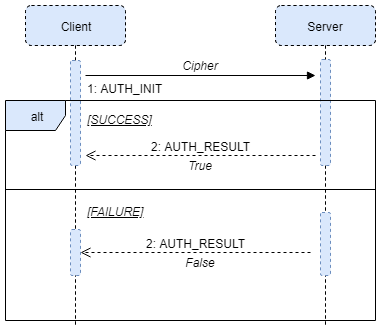
\includegraphics[width=80mm]{Figures/ACS_Prot/Auth_Init}
	  \decoRule
	  \caption[ACS protocol: Authentication]{This shows how the server authenticates the user. If the decrypted cipher matches the expected value, the authentication is successful.}
	  \label{fig:prot_auth}
	\end{figure}

	\subsubsection*{Authentication}
	The authentication is done as described in \Cref{sec:wsprot_auth}. The endpoint encrypts it's e-mail address using the symmetric key, and sends it to the server in the data field of an \emph{Authentication init} packet. The server then decrypts the cipher and compares the e-mail stored to the one received. If there is a match, the authentication is successful. If it does not match the connection is dropped. The result of the authentication is sent as part of the \emph{Authentication reply} packet. See \Cref{fig:prot_auth} for a diagram of this process. 
	
	\subsubsection*{Init}
	Once the endpoint has been authenticated by the server, it is available to receive offers and send offers. This is where the \emph{Init} functionality comes in. This is an offer to send files to an identity. It contains information about who the sender is, who the intended recipient is, and metadata about the file to be shared. See \Cref{fig:ACS_rec} for an example. If the server receives this type of request, it is forwarded to the indicated endpoint. The file metadata can be end-to-end encrypted without impacting the functionality.

	\subsubsection*{Accept}
	Once an endpoint receives an offer to receive files (in the form of an \emph{Init} packet), the user has the choice to accept or refuse the connection. If the user accepts, an \emph{Accept} packet containing a WebRTC Offer is sent back through the ACS server.

	\subsubsection*{Refuse}
	In the same way as explained for the \emph{Accept} functionality, the \emph{Refuse} functionality declines the offer to connect to the other endpoint. It terminates the connection setup between the two identities.

	\subsubsection*{Answer}
	If the Sender receives an \emph{Accept} packet, it means the other endpoint accepted the connection. As such, the Sender processes the WebRTC Offer received, and generates a WebRTC Answer. This is then shared back to the Recipient through the ACS server in the form of an \emph{Answer} packet.

	\subsubsection*{ICE}
	Since this solution utilizes ICE trickling (Described in \Cref{sec:webrtc_icetri}), it needs a protocol to continuously share ICE candidates between the two endpoints. This function exists to allow the sharing of such candidates. In other words, the ICE candidate is attached as the data portion of the \emph{ICE} packet.

	\subsubsection*{Done}
	This functionality indicates that the previous connection, for whatever reason, has ended. If one endpoint sends such a packet to the ACS server, the server should consider both endpoints available for new connections.

	\subsubsection*{Error}
	If for any reason an error occurs on either side, this functionality allows for sharing what went wrong with the other endpoint. As such, the reason for the error is added to the data portion of the packet. There is no requirement to share error messages with the connection partner, but it can be useful in order to discern between an intended pause/stop in the connection, or if something went wrong.

	\subsubsection*{Wait}
	This functionality is primarily aimed at allowing semi-asynchronous communication. It is used as a message to the endpoint from the ACS server, if they try to reach an identity currently connected to another endpoint. This indicates that the intended recipient is busy, but online. If one implements queuing, it can be used to tell the sender to wait until the endpoint is ready and then automatically connect.
%
	%Forwarding
	%
	\subsection{Forwarding}
	The ACS is a service that exclusively forwards information, regardless of whether it is encrypted or not. This is done by having the Sender, Recipient, and type of communication unencrypted. The server needs this information in order to handle the requests, and as such, these fields are left in cleartext. Using this information, the ACS picks the correct functionality and executes it. For most functionality, that means just forwarding the information to the correct endpoint. It does, however, need to authenticate the user and take care of that authentication setup, therefore it supports functionality beyond just forwarding information. While some of the data is unencrypted, it is important to note that the communications channel is encrypted, so an attacker cannot gain access to any of the data.
	
	%
	%Semi-asynchronous transfer
	%
	\subsection{Semi-asynchronous transfer}
	The ACS solution can allow for semi-asynchronous messaging. This means that one can issue the connection request at any time, but wait for it to be handled until the other endpoint comes online. It also allows for a queuing system that stores requests and handles them at the first available opportunity. This still requires the sender to be online, connected to the ACS, and available for transfer. As such, while the actual transfer is synchronous, the request and user interactions are not, thus 'semi-asynchronous'.

	This brought forward the need for the \emph{wait} and \emph{busy} functionality in the protocol, as well as a queue of jobs for each connection, temporarily kept in the ACS server. This type of transfer is not implemented in SendIt, but some of the frameworks and systems needed for such functionality is implemented and ready to be used.
% Chapter 4
%
\chapter{Implementation of SendIt} % Main chapter title
%
\label{Chapter4} % For referencing the chapter elsewhere, use \ref{Chapter1} 
%
In this chapter the implementation specifics of SendIt will be discussed. It will go through how the application looks and functions, how the ACS server is implemented, and finally, how the application can be extended and improved.

\section{Application}
%
  In this section, everything regarding the implementation of the application will be discussed, except the usage modes. It will go through the implementation and usage of SendIt and clearly explain how the different concepts and technology works.
  %
  \subsection{Cryptography}
  \label{sec:crypto_imp}
    In SendIt's implementation, the Web Crypto API (SubtleCrypto module) is used for generating and handling keys \cite{ar_webcrypto}. This allows for an easy and reliable way to standardize the handling of keys, encryption and decryption, in every system. The Web Crypto API is available in most internet browsers. It has been available through the Chrome browser, since the release of version 37 \cite{url_webcr_supp}. Using a pre-developed, and tested API for SendIt's cryptographic functions allows for a more reliable system. Since the implementation of the cryptographic functions and debugging has already been done, it allows more time to be spent on developing other functionality. This is the reasoning for using the Web Crypto API.

    The system begins with creating a unique key pair, if no such key pair already exists. This check is done at the time of choosing to send or receive a file so that, if desired, the user can change to the correct identity for this connection. The key pairs used consists of two RSA-OAEP 2048 bit keys with SHA-1 hashing, but this is easy to change if the need arises. The choice of key-type was based on the recommendation of the WebCrypto API specification \cite{ar_webcrypto}.

    The key-exchange is done over the secure DataChannel created by WebRTCs PeerConnection \cite{ar_webrtc}. Once a key exchange (successful connection) has taken place, the created key pair and the other identity's public key will be written to the disk.

    SendIt imports the file into memory once a key is needed. After which it extracts the keys stored. Once the keys have been used and the communication has finished, SendIt will overwrite the existing file with the new, updated information. The file containing the keys has information exceeding just the known keys. Both the identity associated with a key, and the key itself, has to be stored.

    As discussed in \Cref{sec:crypto_des}, SendIt uses symmetric and asymmetric keys, since asymmetric keys can only encrypt small amounts of data. The maximum amount of data the asymmetric key pair mentioned previously (\emph{RSA-OAEP 2048 bit with SHA-1 hashing}) can encrypt is 214 bytes \cite{PKCSV2RSA2012}. SendIt uses an AES-GCM symmetric key, with a length of 256 bits, which allows for encryption of up to \emph{2\textsuperscript{39}-256} bytes of data \cite{ar_webcrypto}. This is well within the limits of what is necessary in SendIt. 

%
  \subsection{Connection setup}
  \label{sec:conn_set_imp}
  %Connection setup - Offer&Answer generation & Processing
    This section will explain the functionality of generating the connection information and how each endpoint processes that information in order to create the connection. SendIt implements two different ways to share the connection information, in order to create a P2P connection between two endpoints. These two modes will be explained in \Cref{Chapter5}.

    %Offer / Answer generation
    The Offer and Answer generation and processing is done as described in \Cref{sec:webrtc}. The difference from the normal usage is that they can also be encrypted before being transferred, which means they have to be decrypted before being used. The original form of the data is a JavaScript object.

    To encrypt the data, it is first turned into a string, then to an ArrayBuffer, after which it is encrypted. To decrypt the data, it is converted from a string to an array of integers. It is then converted to an Uint8Array before being decrypted. The decrypted data is also an Uint8Array, which is turned into a string, and then back into a JavaScript object. All the conversions just mentioned, stem from the different data formats required by the different libraries and frameworks. For more information on how the data is exchanged, see \Cref{Chapter5}.

    %ICE and SDP? How and waht differs?
    The actual setup of the connection and the creation of the DataChannel is done according to the examples and descriptions in \Cref{sec:webrtc}. The only difference in connection setup between the two modes, is if ICE trickling is used or not.

    When the Offer and Answer is successfully exchanged, a direct connection is created. There are scenarios, when this is not case. Known causes of issues with completing the connection are:
    %
    \begin{itemize}
      \item Setup not completed within a certain time frame (see \Cref{Chapter6})
      \item One or both endpoints are behind symmetrical NAT
      \item One or both endpoints change network location (For example, connect to a different network.)
    \end{itemize}
    %

    When implementing SendIt, the choice was made to not support symmetrical NAT, as it requires a TURN server. This means the connection would no longer be a direct end-to-end connection. 
    Widespread use of IPv6 would solve this issue, as it would eliminate the need for NAT traversal and TURN servers. As for changes in network conditions, there is nothing to be done on the application side, except including a signaling server. As such, the system assumes that users will stay in the same network conditions for the duration the connection is active. For the ACS mode, automatic reconnection is an option which can be added as an extra feature.
  
  \subsection{File transfer functionality}
    %Chunking & Size limit
    The communication will consist mostly of file data, and as such, it is interesting to know how much data can be handled. In theory, splitting files into chunks during reading, and then transferring these chunks, allows for infinitely large transfers. The default max size for Node.js is approximately 1 GB for 32-bit machines, and 2 GB for 64-bit machines. This indicates the maximum amount of data that can be kept in memory. The reason for this limit is because this is the max amount of data the V8 JavaScript engine used by Node.js can have in memory at the time \cite{url_node,url_v8}.

    The current functionality separates each file into chunks of 1200 bytes, as is the limit imposed by the Chromium implementation of WebRTC \cite{SctptransportCcCode}. The max file size is set to 160 megabytes during development, since it was the max size used by PubShare \cite{url_pubshare}. It is likely that this can be increased without any issues, since Node.js has support for keeping larger files in memory, but it would require some testing before being ready to deploy. See \Cref{fig:file_off} for an illustration of the previous explanation.

  \subsection{Programming languages, libraries and frameworks}
    SendIt is developed in JavaScript utilizing the Electron framework. These technologies were chosen because they allow for easy implementation, while supporting multiple operating systems. Easy connection setup and direct communication via P2P is also available, through pre-developed and tested frameworks. In addition, it also allows for the use of existing libraries and standardizations developed for web browsers, in desktop applications. 

    To clarify, this means that the user does not need to open their web browser to utilize SendIt, but can install it and run it like they would run any desktop program with a GUI. It also allows for easy creation of an installer file, which means the end user only needs to download and run the installer, for the program to be usable.

    %
    \begin{figure}
    \centering
    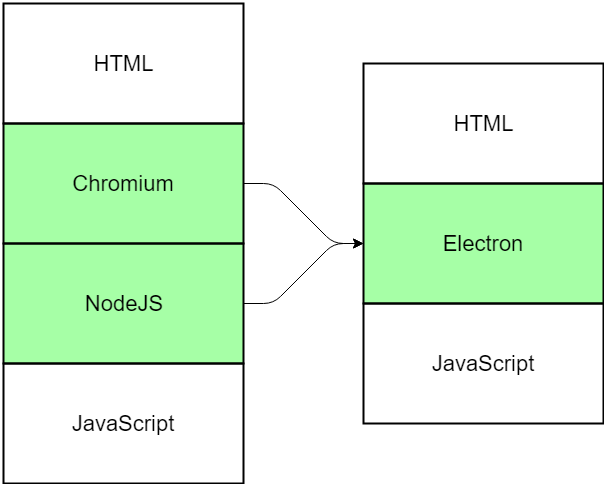
\includegraphics[width=60mm]{Dev_Stack_New}
    \caption[Application stack]{The stack for the prototype application. It is built using HTML, Electron, and JavaScript.}
    \label{fig:dev_stack}
    \end{figure}

    The electron framework uses Node.js for the back end and Chromium for the front end \cite{url_electron}. In practice, this means that the system is built on: HTML, Electron and JavaScript, where Electron utilizes Chromium and Node.js. (see \Cref{fig:dev_stack}) This allows us to use modules and frameworks from any of the previously mentioned entities independently. Our implementation uses these libraries and frameworks:
    %
    \begin{itemize}
    \item Node.js API - Used for reading and writing to the disk and finding correct files and folders \cite{url_node}.
    \item Chrome Web Cryptography API - Used to handle the creation and exportation of keys, encryption, and decryption \cite{ar_webcrypto,url_webcr_supp}.
    \item Node.js Clipboardy - Utilized to automatically copy the generated Offer/Answer to the clipboard \cite{url_clipboardy}.
    \item Node.js Electron-prompt - Used to create pop-ups for requesting user input \cite{url_ele-prompt}.
    \item Chrome Native WebRTC - Used for creating and managing WebRTC connections \cite{url_webrtc_chrome}.
    \item jQuery v3.2.1 - Utilized to manage front end actions and dynamic updates \cite{url_jQuery}.
    \item Bootstrap v3.3.7 - Used to manage front end modules and dynamic updates \cite{url_bootstrap}.
    \end{itemize}
    %

  %
  \subsection{Program flow}
  \label{sec:progflow}
  %Program Flow
  The general appearance of the program will be explained in the following section. The functionality which is unique to each mode will be discussed in \Cref{Chapter5}. That means that most of the actual functionality is not explained here, but rather the installation, setup, and settings available. In addition, it will also explain the screens not related to the connection setup. These include the waiting screen, the transfer status screen, and the transfer complete screen.
  %
    \subsubsection*{Installation and launching application}
    %Installation and launch
      %Screenshots and explanation
    The application comes in the form of installer files for Linux, Mac, and Windows. These files are in the format of \emph{.deb} for Linux, \emph{.dmg} for Mac, and \emph{.exe} for Windows. The installers are very basic and require no interaction except executing them. After that is done, the image shown in \Cref{fig:inst} will appear and display a small animation. Afterwards, SendIt is installed and will be available. In most cases, the icon will be available on the desktop. Once the application is launched for the first time, a pop-up window will appear, as indicated in \Cref{fig:popup}. Afterwards, the user is taken to the Home screen. This pop-up window will only be displayed the first time the program is opened.
    \begin{figure}[H]
      \centering
      
\includegraphics[width=60mm]{Figures/Base/installer}
      \decoRule
      \caption[SendIt: Install animation]{While the installation of SendIt is ongoing, this small box, with basic animations, will appear. Once it disappears, the program is installed.}
      \label{fig:inst}
    \end{figure}

    \begin{figure}[H]
      \centering
      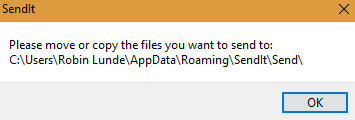
\includegraphics[width=80mm]{Figures/Base/start_up}
      \decoRule
      \caption[SendIt: First launch pop-up]{This pop-up appears the first time the program is started. It informs the user of the default location of the upload folder. The files the user wants to send should be placed in this folder.}
      \label{fig:popup}
    \end{figure}  
    %
  \subsubsection*{Home screen}
  %Home screen
    %Screenshot & explanation. Include popup!
  The Home screen is the first screen the user sees. On this screen, there is not much detail or information. The logo and acronym for SendIt is displayed, as well as the navigation bar. From here on, it is all about choosing the desired functionality or tweaking the settings to fit the users desire. The only difference between the Home screen for the two modes, is the formatting of the word 'Serverless' at the bottom of the screen, as well as the ACS mode not having a receive button on the navigation bar.
    \begin{figure}[H]
      \centering
      
\includegraphics[width=\textwidth]{Figures/Base/Home_Screen}
      \decoRule
      \caption[SendIt ACS mode: Home screen]{The Home screen displayed when the application is in ACS mode. The navigation bar has no button for receiving files. The 'Serverless'-part of SendIt's acronym is also crossed out, at the bottom of the page.}
      \label{fig:hs_acs}
    \end{figure}

    \begin{figure}[H]
      \centering
      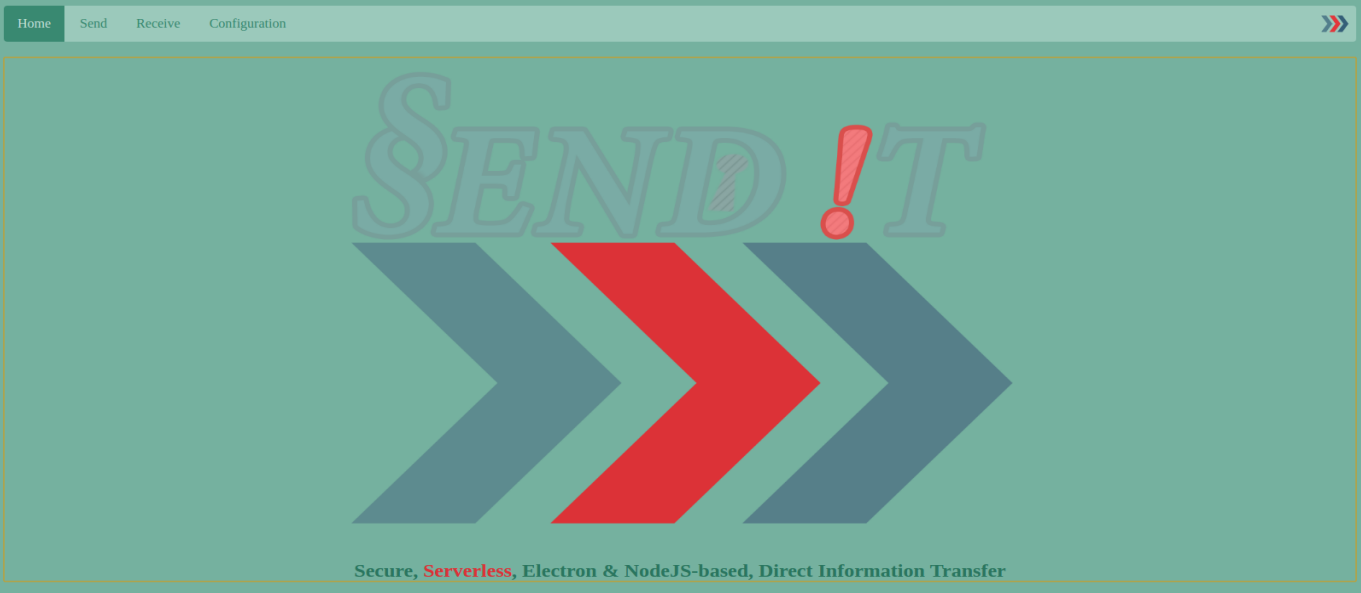
\includegraphics[width=\textwidth]{Figures/Base/Home_Screen_SL}
      \decoRule
      \caption[SendIt Serverless mode: Home screen]{The Home screen displayed when the application is in Serverless mode. The navigation bar has a button for both sending and receiving files.}
      \label{fig:hs_sl}
    \end{figure}

  \begin{figure}[H]
      \centering
      
\includegraphics[width=\textwidth]{Figures/Base/navbar_sl}
      \decoRule
      \caption[SendIt: Navigation bar]{The navigation bar displayed in Serverless mode. The receive-button is not present in the ACS mode, since a separate page will be displayed if someone offers to send file(s) to you. This bar is always displayed at the top of the window.}
      \label{fig:hs_nb}
    \end{figure}
  %
  \subsubsection*{Settings}
  %Settings screen
    %Screenshot and explanation.
    The base view of the settings page is represented in \Cref{fig:sett}. At the top one can input which identity (or e-mail address if you will) to use. Further down, one can remove the configuration file, the file which stores all the data about which identity and which settings to use. Following are radio buttons, where one can choose which mode to use and if one wants to use custom locations, for example, where to store downloaded files. At the bottom, information about the current settings are displayed. Finally, there is a 'save changes' button, to store the changes made.

    In \Cref{fig:set_det}, more detailed options are displayed. These appear when clicking the non-default option of the radio buttons. If the ACS option is selected for \emph{Mode selection}, the field for indicating the address of the server is displayed, as well as a 'save' button and a 'reset' button. Afterwards, there is an option for manually selecting a file from which to load keys. One can also remove the file currently used, by pressing the 'remove ALL current keys!' button or remove individual keys by clicking on the corresponding e-mail address. Finally, one can customize the download and upload folder location.
    %Base screen
    \begin{figure}[H]
      \centering
      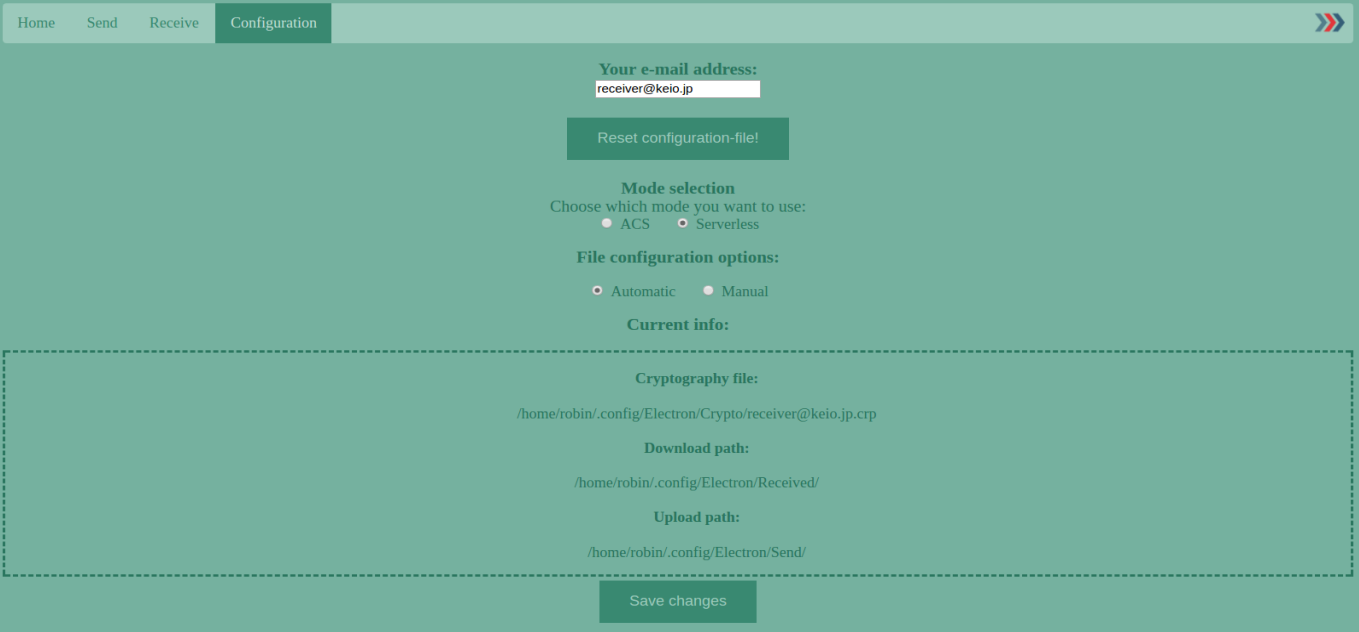
\includegraphics[width=\textwidth]{Figures/Base/Settings}
      \decoRule
      \caption[SendIt: Settings screen]{The screen used for indicating user preferences, upload and download locations, identity management, and mode selection.}
      \label{fig:sett}
    \end{figure}

    %Details screen
    \begin{figure}[H]
      \centering
      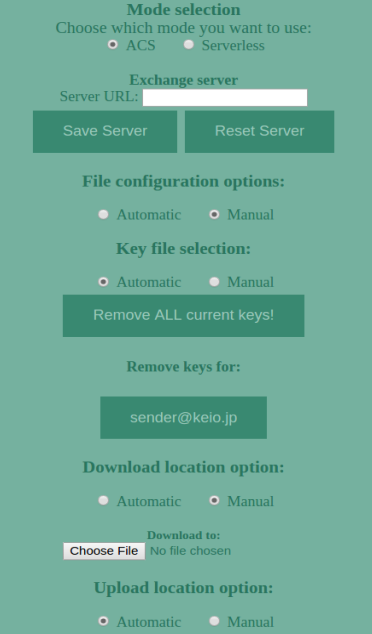
\includegraphics[width=70mm]{Figures/Base/settings_expanded}
      \decoRule
      \caption[SendIt: Detailed settings screen]{The expanded version of the settings screen with the selections and menus displayed.}
      \label{fig:set_det}
    \end{figure}

  \subsubsection*{After successful connection setup}
  \label{sec:file_recv}
  %
    All the following examples are taken from the Serverless mode, but they look identical in the ACS mode, with the exception of the navigation bar. These are the different screens shown once the endpoint has completed their part of the connection setup exchange.\\
     
    \noindent
    \underline{Waiting screen}\\
    The waiting screen is displayed while the endpoints are waiting for WebRTC to establish the P2P connection.
    \begin{figure}[H]
      \centering
      
\includegraphics[width=\textwidth]{Figures/Base/waiting}
      \decoRule
      \caption[SendIt: Waiting for connection screen]{This screen is displayed while waiting for the endpoints to connect via P2P (WebRTC).}
      \label{fig:SL_wait}
    \end{figure}

    %
    \noindent
    \underline{Transfer screen}\\
      It displays details about the current file being transferred; it's name and type, as well as the total number of files to transfer. It also shows the percentage of data transferred for the current file. Finally, there is a cancel button in case one end wants to stop the transfer.
    \begin{figure}[H]
      \centering
      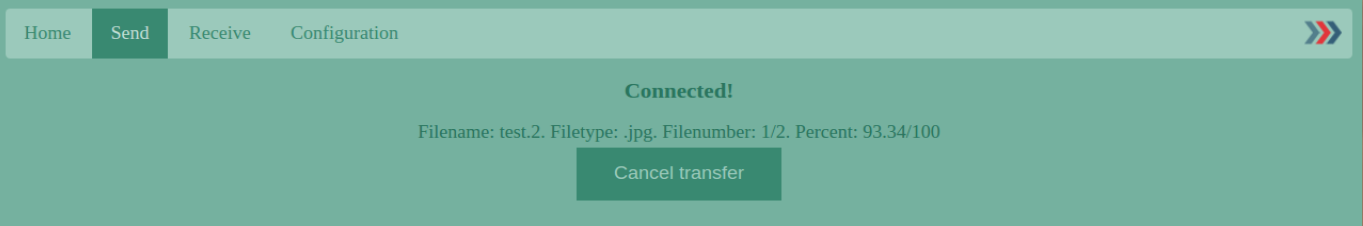
\includegraphics[width=\textwidth]{Figures/Base/transfer}
      \decoRule
      \caption[SendIt: Transfer screen]{This screen displays details about the status of the current transfer.}
      \label{fig:SL_trans}
    \end{figure}

    %
    \noindent
    \underline{Connection completed screen (\emph{Sender})}
    \begin{figure}[H]
      \centering
      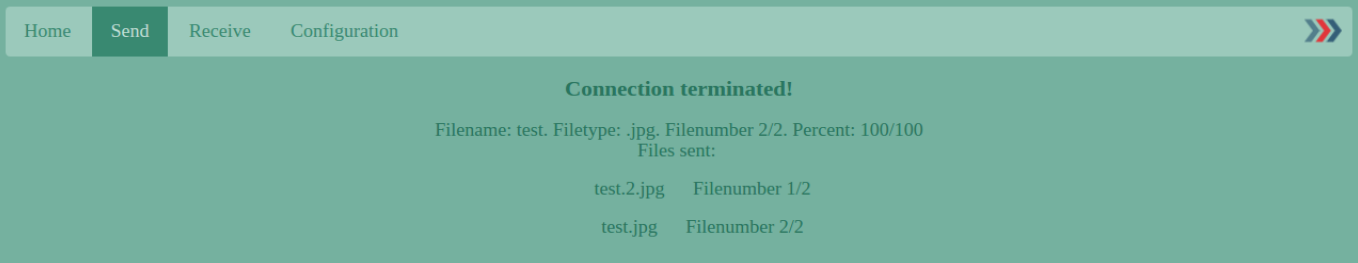
\includegraphics[width=\textwidth]{Figures/Base/sender_complete}
      \decoRule
      \caption[SendIt: Final screen (Sender)]{This screen displays details about which files were transferred.}
      \label{fig:SL_rec1}
    \end{figure}

    %
    \noindent
    \underline{Connection completed (\emph{Receiver})}
    \begin{figure}[H]
      \centering
      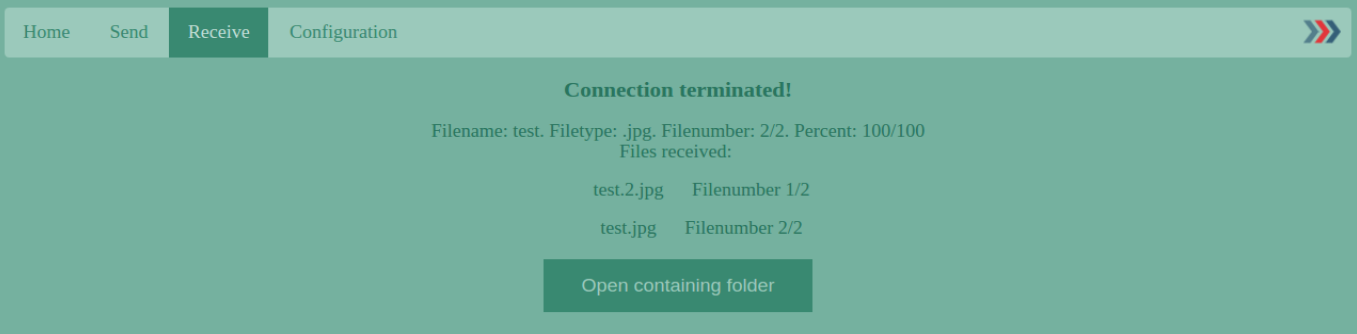
\includegraphics[width=\textwidth]{Figures/Base/receiver_complete}
      \decoRule
      \caption[SendIt: Final screen (Receiver)]{This screen displays details about which files were received. It also has an 'open containing folder'-button for easy access to the received files.}
      \label{fig:SL_rec2}
    \end{figure}
%
\section{ACS server implementation}
\label{sec:acs_serv_imp}

  The ACS server is implemented in JavaScript, using the Node.js environment. It uses a library implementing the Web Crypto API for Node.js \cite{WebcryptoW3CWeb2018}, which allows for the use of the same keys, the same encryption scheme and generally the same cryptographic solutions as in the application. This makes it easy to use and means there is no need for developing support for, or using other cryptographic methods, to authenticate with the ACS server.

  \subsection{WebSockets}
  \label{sec:acsws}
  %WS
    %How is it used, secure, advantage
    %IMPLEMENTATION
    All communication between endpoints and the ACS server is done over WebSockets using HTTPS. This enables bi-directional communication at any time and creates an easy interface to use for communicating with different endpoints. The communication is exclusively done using the protocol described in the next section.
    
    The WebSocket interface and API also allows for easy handling and management of clients. Clients can connect and disconnect randomly without affecting the service as a whole. All clients are treated equally and it is easy to address each client individually. Because of this, it is very easy to receive information from one client and immediately forward it to the intended recipient. 

  \subsection{Protocol}
  \label{sec:prot_imp}
  This section reviews the implementation of the protocol discussed in \Cref{sec:wsprot}. For an overview of the packet format, see \Cref{tab:basic}. The format indicated for each of these packets, goes in the data field of the general packet format. Following is the practical implementation of the protocol.
  %
  \subsubsection*{Lookup}
 %
  The \emph{Lookup} packet from client to server does not contain any data. The packet sent from the server to the client can contain the data indicated in \Cref{tab:lookup}. If \emph{res} is \emph{true}, the data will consist of the fields \emph{res}, \emph{wrap} and \emph{key}. The \emph{wrap} field consist of the symmetric key, encrypted with the other endpoint's public key. If \emph{false}, it will consist of \emph{res} and \emph{key} only.
%
  \begin{table}
    \caption[ACS protocol: Lookup packet]{Lookup packet}
    \label{tab:lookup}
    \centering
    \begin{tabular}{l l l l}
      \tabhead{Name} & \tabhead{Type} & \tabhead{Argument details} & \tabhead{Required} \\
      \midrule
      res & Boolean & Indicates if authentication setup is needed or not & Yes\\
      key & JWK & Server's public key in JWK format & Yes\\
      wrap & Array & Encrypted symmetric key& No\\
      \bottomrule\\
    \end{tabular}
  \end{table}
%
  \subsubsection*{Authentication setup}
  %
  The possible arguments used by the Authentication setup and Authentication Setup Reply functionality are shown in respectively \Cref{tab:auth_set} and \Cref{tab:auth_s_r}. The public key of the client is sent to the server. The server tries to set up authentication for subsequent connections. The authentication setup is considered a success if no previous data is stored for this e-mail or public key. If this is the case, the \emph{Authentication Setup Reply} packet will contain \emph{res} and \emph{wrap}, where \emph{res} is set to \emph{true}. The \emph{wrap} field consists of the symmetric key, encrypted with the other endpoint's public key. If the setup fails, the \emph{wrap} field is not included.
%
  \begin{table}
    \caption[ACS protocol: Authentication Setup packet]{Authentication Setup packet}
    \label{tab:auth_set}
    \centering
    \begin{tabular}{l l l l}
      \tabhead{Name} & \tabhead{Type} & \tabhead{Argument details} & \tabhead{Required} \\
      \midrule
      key & JWK & Client's public key in JWK format & Yes\\
      \bottomrule\\
    \end{tabular}
  \end{table}
%
  \begin{table}
    \caption[ACS protocol: Authentication Setup Reply packet]{Authentication Setup Reply packet}
    \label{tab:auth_s_r}
    \centering
    \begin{tabular}{l l l l}
      \tabhead{Name} & \tabhead{Type} & \tabhead{Argument details} & \tabhead{Required} \\
      \midrule
      res & Boolean & Authentication result & Yes\\
      wrap & Array & Encrypted symmetric key& No\\
      \bottomrule\\
    \end{tabular}
  \end{table}
%
  \subsubsection*{Authentication}
  %
  \Cref{tab:prot_auth} and \Cref{tab:prot_auth_rep} shows the possible arguments for the authentication packets. The \emph{ciph} field contains the client's email address, encrypted with the symmetric key. The \emph{Authentication Result} packet returns a boolean value directly in the data field, indicating the result of the authentication process. Successful authentication returns \emph{true}.
%
  \begin{table}
    \caption[ACS protocol: Authentication packet]{Authentication packet}
    \label{tab:prot_auth}
    \centering
    \begin{tabular}{l l l l}
      \tabhead{Name} & \tabhead{Type} & \tabhead{Argument details} & \tabhead{Required} \\
      \midrule
      ciph & Array & Client's encrypted e-mail address & Yes\\
      \bottomrule\\
    \end{tabular}
  \end{table}
%
  \begin{table}
    \caption[ACS protocol: Authentication Result packet]{Authentication Result packet}
    \label{tab:prot_auth_rep}
    \centering
    \begin{tabular}{l l l l}
      \tabhead{Name} & \tabhead{Type} & \tabhead{Argument details} & \tabhead{Required} \\
      \midrule
      - & Boolean & Authentication result & Yes\\
      \bottomrule\\
    \end{tabular}
  \end{table}
 % 
  \subsubsection*{Init}
  %
  The \emph{Init} packet can consist of the data shown in \Cref{tab:init}. It contains information about the files being offered. Each object in the \emph{files} array has information about the file name, file type and the size of the file.

   \begin{table}
    \caption[ACS protocol: Initiate Connection packet]{Initiate Connection packet}
    \label{tab:init}
    \centering
    \begin{tabular}{l l l l}
      \tabhead{Name} & \tabhead{Type} & \tabhead{Argument details} & \tabhead{Required} \\
      \midrule
      files & Array & Array of objects with file data & Yes\\
      \bottomrule\\
    \end{tabular}
  \end{table}
%
  \subsubsection*{Accept}
  %
  The \emph{Accept} packet contains the WebRTC Offer generated and indicates that the endpoint wants to receive the data previously offered. The WebRTC Offer can either be encrypted or in cleartext. See \Cref{tab:acc} for more information about the data transferred. If the Offer is sent in cleartext, the data transferred is just the WebRTC Offer object. If not, the data consists of the other three fields (\emph{wrap}, \emph{iv}, and \emph{ciph}). The \emph{wrap} field consists of the symmetric key, encrypted with the other endpoint's public key. The \emph{ciph} field consists of the WebRTC Offer, encrypted with the symmetric key.

  \begin{table}
    \caption[ACS protocol: Accept packet]{Accept packet}
    \label{tab:acc}
    \centering
    \begin{tabular}{l l l l}
      \tabhead{Name} & \tabhead{Type} & \tabhead{Argument details} & \tabhead{Required} \\
      \midrule
      - & Object & The WebRTC Offer generated by the endpoint & No\\
      wrap & Array & Encrypted symmetric key & No\\
      iv & Array & Initialization vector for the symmetric key & No\\
      ciph & Array & Encrypted WebRTC Offer & No\\
      \bottomrule\\
    \end{tabular}
  \end{table}
  %
  \subsubsection*{Refuse}
  The refuse packet contains no data. If this packet is received the connection setup is stopped.
%
  \subsubsection*{Answer}
%
 The \emph{Answer} packet contains the WebRTC Answer generated by the endpoint. The WebRTC Answer can either be encrypted or in cleartext. See \Cref{tab:ans} for more information about the data transferred. If the Answer is sent in cleartext, the data transferred is just the WebRTC Answer object. If not, the data consists of the other two fields (\emph{iv} and \emph{ciph}). The \emph{iv} field consists of the initialization vector, encrypted with the other endpoint's public key. The \emph{ciph} field consists of the WebRTC Answer, encrypted with the symmetric key.
 %
\begin{table}
    \caption[ACS protocol: Answer packet]{Answer packet}
    \label{tab:ans}
    \centering
    \begin{tabular}{l l l l}
      \tabhead{Name} & \tabhead{Type} & \tabhead{Argument details} & \tabhead{Required} \\
      \midrule
      - & Object & The WebRTC Answer generated by the endpoint & No\\
      iv & Array & Encrypted initialization vector for the symmetric key & No\\
      ciph & Array & Encrypted WebRTC Answer & No\\
      \bottomrule\\
    \end{tabular}
  \end{table}
%
  \subsubsection*{ICE}
%
  This packet contains the data showed in \Cref{tab:ice}. The data can either be encrypted or sent in cleartext. If it is not encrypted, it will be sent as an ICE candidate object. If it is encrypted, it will consist of the fields \emph{ciph} and \emph{iv}. The \emph{ciph} field consists of the ICE candidate, encrypted with the symmetric key.
%
  \begin{table}
    \caption[ACS protocol: ICE packet]{ICE packet}
    \label{tab:ice}
    \centering
    \begin{tabular}{l l l l}
      \tabhead{Name} & \tabhead{Type} & \tabhead{Argument details} & \tabhead{Required} \\
      \midrule
      - & Object & The ICE candidate generated by the endpoint & No\\
      ciph & Array & Encrypted ICE candidate & No\\
      iv & Array & Initialization vector for the symmetric key & No\\
      \bottomrule\\
    \end{tabular}
  \end{table}
%
  \subsubsection*{Done}
%
  The \emph{done} packet contains no data, and indicates that the connection is terminated and that the endpoints are ready for a new connection.
%
  \subsubsection*{Error}
%
  The \emph{error} packet can contain data about which error occurred. If the server receives an \emph{error} packet with an indicated destination, it will forward it to the correct endpoint. The data will have the format indicated in \Cref{tab:err}.
%
  \begin{table}
    \caption[ACS protocol: Error packet]{Error packet}
    \label{tab:err}
    \centering
    \begin{tabular}{l l l l}
      \tabhead{Name} & \tabhead{Type} & \tabhead{Argument details} & \tabhead{Required} \\
      \midrule
      - & String & Error details & No\\
      \bottomrule\\
    \end{tabular}
  \end{table}
%
  \subsubsection*{Wait}
%
  The \emph{wait} packet does not contain data. It indicates that an endpoint is busy, and, as such, cannot partake in a connection at this time. If a destination is specified, the server forwards the packet to the correct endpoint.
%
\section{Extendability and improvements}
%
In this section the extendability of SendIt, in general, will be assessed. SendIt can be used as a platform to build extended functionality, and as such, it should be noted in what way this can be done, and how one stands to benefit from doing it. It will also discuss possibilities for improving the current implementation.

  \subsection{Key storage encryption}
  %
    The file where keys are stored should be encrypted and password protected, or otherwise access restricted. The key file should only be usable if the correct password is provided. If the wrong password is provided, the keys should not be accessible. The key file should be updated every time it is used by the system. This will allow users to change the password used to access the keys between each use and also make it easy to update information regarding each key. In addition, it gives no guarantee that the same encryption is used each time, which makes attacks over time harder to execute, since there is no reliable way to analyze changes or patterns in the way the file is stored. This functionality should be implemented and would improve the solution. It is not currently implemented in SendIt, due to time constraints. 

  \subsection{E-mail verification}
  %E-mail verification
    One way to extend the current functionality is to add e-mail verification to the process of registering an identity. This would increase the trustworthiness of each identity since proving ownership of the registered e-mail address would be a necessity. It would however, also include all the issues stemming from how the e-mail system is implemented. It would also make the registration process harder and require more from the users before being able to use the system. Because of these issues, it is not included in the system by default, but can easily be added. It is left up to the end users to develop and extend the proposed system, if such functionality is desired.

  \subsection{Support for bigger files}
  \label{sec:bigfile}
  %
    Supporting bigger files can be achieved by reading in chunks of the file. Then, once a chunk is completely transferred, the next chunk is read into memory. This will allow both endpoints to handle smaller amounts of data at a time, while still having transmitted the whole file after the transfer of all chunks have been completed. It is not recommended to implement this until after the 'resume transfer' feature is implemented, as transferring large amounts of data, without any way of resuming it in case of failure, is less than optimal.

  \subsection{Resume transfer}
  \label{sec:res_trans}
    %
    \begin{table}
      \caption[Record of communication]{Fields included in the record of communication.}
      \label{tab:comm_rec}
      \centering
      \begin{tabular}{cccc}
            \textbf{Sender} & \textbf{File(s)} & \textbf{Date} & Completed \\
            \midrule
            test@email.com & picture.jpg & 2018-03-20 & 0\\
            another@email.com & document.doc & 2018-05-13 & 4\\
            \bottomrule
      \end{tabular}\\
    \end{table}
    %
    This functionality can easily be implemented based on a communication record. Since every identity will have a list of previously transferred files, it will have the file name included. If the transfer is not completed, this record can store information about which chunk of the file was the last to be received, and the endpoint can request the transfer to be continued from there.

    If the sender is not willing to resume the previous transfer, it can either start over, or the sender can offer to transfer another file. This decision is up to the sender's settings and/or preference. If the sender choses to not resume the transfer, the data previously stored on the receiver's local system should be removed, and the record updated as a failed transfer. The system should only allow for the requested file to be shared on the subsequent connection. 

    To clarify: Alice tries to send Bob \emph{File A}, but the connection is broken. If Alice tries to send \emph{File A} again, it will resume from the last chunk received. If it fails again, it will also allow for the transmission of \emph{File A} to be resumed. However, if Alice contacts Bob again, but tries to send \emph{File B} this time, the previously transmitted information (\emph{File A}) stored by Bob should be removed.

    The record of communications can be implemented by creating a log that contains the fields indicated in \Cref{tab:comm_rec}. The last field can either be \emph{-1} (meaning failed), \emph{0} (meaning success) or the number of the last received chunk. This is useful for being in compliance with the GDPR, allowing the user to keep track of their interactions for reviewing their activity, and implementing a 'resume transfer' functionality, as mentioned.

  \subsection{WebRTC IDP inclusion}
  %WebRTC IDP
    WebRTC comes with a suggested standard for implementing Identity Provider services. An Identity Provider is a trusted third party that corroborates an identity. An example would be connecting ones Facebook account to an identity, as a means for other endpoints to verify the authenticity of that identity. This is possible for many different services and can be a means of increasing trust in identities. Currently, there are some arguments and disagreements on how this should be implemented in WebRTC, and as such, there are very few existing frameworks that can be used. This is expected to change, and at that point, using these services will allow for an easier way to increase trust in endpoints.

    The trust is of course reliant on the end user already trusting the service that is used as the Identity Provider, and that the identity is as expected. For example:\\
    If the Identity Provider used is a known service (such as Facebook), one can reasonably trust the data received. If it is from a service unknown to the user, then the identity provision does not increase the trust at all, since the data may be created for malicious purposes. In the same way, if the endpoint is expecting to be communicating with Alice, but Bob's identity is asserted by the provider, the end user should be sceptical.

    In summary, this functionality would allow one to link accounts from other, independent services with their WebRTC connection, in order to corroborate the endpoint's identity and increase trust.

  \subsection{SendIt as a platform}
  %
    This is an interesting idea since the proposed system allows for connection setup and identity assertion. One can use SendIt for this functionality and build any kind of additional functionality on top, if so desired. Especially combining with VOIP, which WebRTC is often used for, can be useful. It allows the developers to focus on their services and additional functionality, while allowing the easy to use and secure setup offered by SendIt to take care of identity management and authentication. The design and implementation of SendIt is modular, which means one can easily pick and choose which functionality one wants to utilize, and discard the rest. This makes it easy to take advantage of the wanted functionality, while not complicating the solution by including the functionality that is not useful to the specific scenario at hand. 
% Chapter 5
%
\chapter{Operation modes} % Main chapter title
%
%4. Specific design
	%Serverless
		%Use Case
		%Program Flow
		%Specific implementation (of technology)

	%Assisted connection setup
		%Use Case
		%Program Flow
		%Specific implementation (of technology)

\label{Chapter5} % For referencing the chapter elsewhere, use \ref{Chapter1} 
%
In this chapter the in-depth design and functionality of SendIt will be discussed. The program flow and use of the application will be illustrated and the two different modes will be contrasted and compared.

SendIt consists of two modes: Serverless and Assisted Connection Setup (ACS). The difference between these modes is how the setup of the connection is completed, as illustrated in \Cref{fig:mode_comparison}. This affects the flow of the program and also impacts how easy it is to use. In the following sections, the differences will be clearly shown and suggestions on how to best utilize the system will be given. It is important to note that neither mode changes the required technical knowledge to use the program - only the interactions required. This is to make sure all users can utilize both modes.

%
\begin{figure}
	\centering
	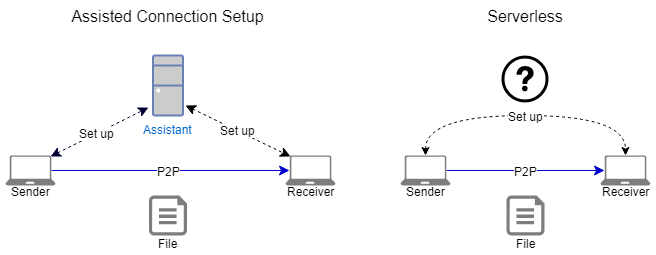
\includegraphics[width=\textwidth]{Figures/SendIt_mode_comparison}
	\caption[SendIt mode comparison]{Left: Assisted Connection Setup mode, Right: Serverless mode} \label{fig:mode_comparison}
\end{figure}

%
\section{Serverless mode}
%
Serverless mode is a mode completely independent of servers (as the name indicates) when establishing the connection. This mode allows the users to be unpredictable in how the Offer and Answer exchange is done and maximizes the improved security of SendIt. It does, however, slightly lower the ease of use and requires more from the end user.
%
\subsection{Use case}
%
As indicated previously, the use case for this mode is by and large for those who value security over usability. This mode should be used if you are already having a conversation with the other endpoint and can quickly take care of the connection setup. Say Alice is talking to Bob and wants to transfer a file. Alice and Bob then take care of the connection setup using an instant messaging service. This allows for a quick and easy file transfer, while getting the added bonus of having the file transferred in a very secure manner. Another example is if Bob wants to transfer an extremely sensitive file to Alice. They can then make a plan on what time they are to do the transfer, in order to be able to take care of the connection setup quickly. This way the file transfer is done with the highest level of security achievable in the system.

As illustrated above, at the cost of some of the usability this mode gives full control to the end user as to how the sharing of the Offer and Answer is done. It does require more manual interactions as well as more planning. This is because the lifetime of the Offer and Answer exchange is short, and as such, puts a time limit on the exchange. It is also because the user has to manually transfer the Offer/Answer generated by their own application and manually input the Offer/Answer received from the other endpoint. There is no change in the technical knowledge requirements to use this mode, just the time constraint and manual interactions as mentioned previously.
%
\subsection{Program flow}
%
The program flow is explained from after the functionality is chosen. For information about functionality other than Send and Receive, see the explanation in \Cref{sec:progflow}.
The program flow of the Serverless mode varies depending on if the user is taking the role of Sender or Receiver. As such, the next section will take you through the two different roles, the choices and screens showed, as well as what is going on. If the user has not yet chosen an identity, this screen will always be the first to appear after choosing the intended functionality (\emph{Send/Receive}):
\begin{figure}[H]
  \centering
  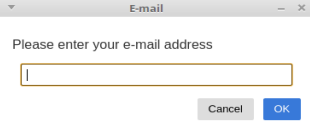
\includegraphics[width=60mm]{Figures/SL/pop_up_own}
  \decoRule
  \caption[Serverless mode: Register identity screen]{This screen displays a pop-up forcing the user to choose which identity (e-mail) to use.}
  \label{fig:serv_popown}
\end{figure}

%If user not stored, username required!

\subsubsection*{Sender:}
%
\noindent
\underline{First screen}
\begin{figure}[H]
  \centering
  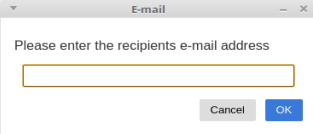
\includegraphics[width=60mm]{Figures/SL/send_pop_up}
  \decoRule
  \caption[Serverless mode: Register recipient screen]{This screen displays a pop-up forcing the user to input the Recipient's identity (e-mail).}
  \label{fig:serv_s_pop}
\end{figure}
%1.1 Input recipients email
%	Required for encryption and authentication

%
\noindent
\underline{Second screen}\\
On this screen, an empty white box appears. Once the Offer is ready, it will appear in the box along with a notification informing the user that it has been copied to the clipboard automatically. The Offer can either be in cleartext or encrypted. Underneath, there is data about which file(s) are to be transferred. It also indicates the file in red if it is not included in the transfer. Finally, there is a continue button that is only clickable after the Offer has been shown.
\begin{figure}[H]
  \centering
  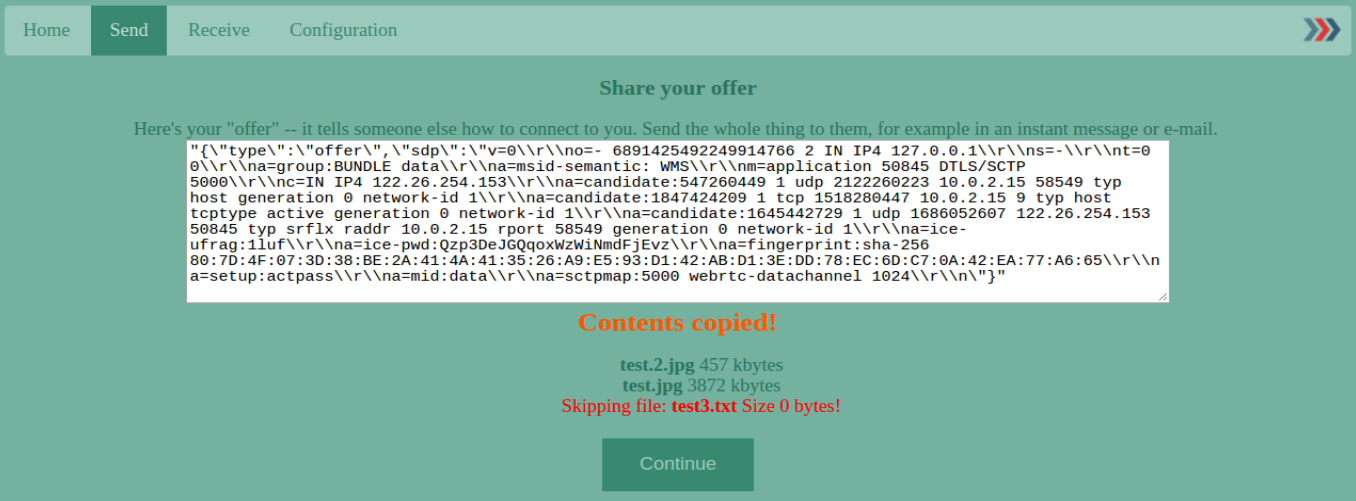
\includegraphics[width=\textwidth]{Figures/SL/offer}
  \decoRule
  \caption[Serverless mode: Display Offer screen]{This screen displays the Offer and the file(s) to be shared. The user should share this Offer with the intended Recipient.}
  \label{fig:serv_s_off}
\end{figure}
	%1.2 send screen - show Offer details, files to send \& recipient
	%-> Share with other user
	%	Displays the files ready for transfer: Name, type, size. After a short delay, the Offer will appear in the box. Either encrypted (if previous communication has happened.) or in cleartext (If first time communicating). This is automatically copied to clipboard. Press continue once Offer has been shared.

%
\noindent
\underline{Third screen}
\begin{figure}[H]
  \centering
  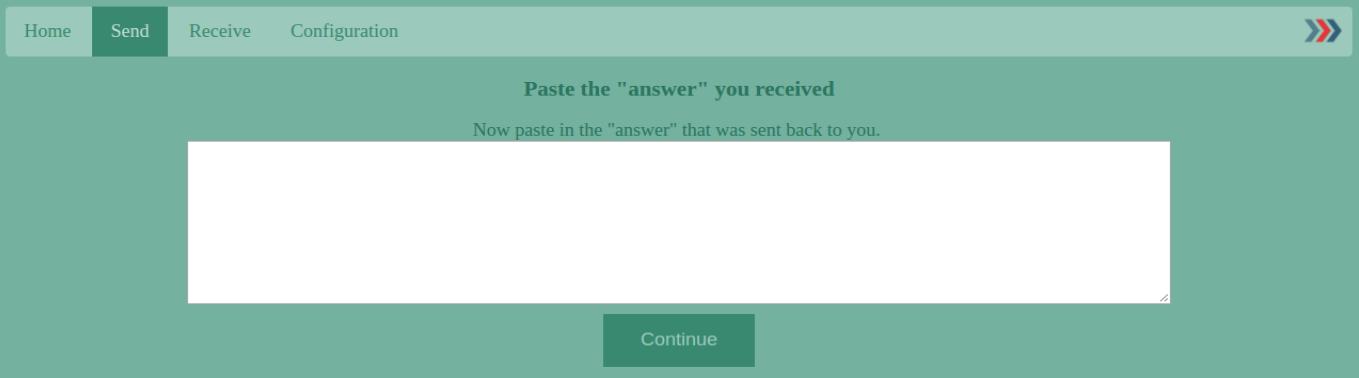
\includegraphics[width=\textwidth]{Figures/SL/sender_answer}
  \decoRule
  \caption[Serverless mode: Input Answer screen]{This screen displays another white box where the user should paste the Answer received from the Recipient. The continue button is only clickable after some information has been entered into the box.}
  \label{fig:serv_s_ans}
\end{figure}
%2 Answer screen - input Answer
%		Displays a box where the user should paste the Answer received from the other endpoint. Once done, click the continue button
	%
\pagebreak
%
\subsubsection*{Receiver:}

%
\noindent
\underline{First screen}
\begin{figure}[H]
  \centering
  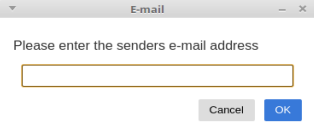
\includegraphics[width=60mm]{Figures/SL/receiver_pop_up}
  \decoRule
  \caption[Serverless mode: Register Sender screen]{This screen displays a pop-up forcing the user to input the Sender's identity (e-mail).}
  \label{fig:serv_r_pop}
\end{figure}

%
\noindent
\underline{Second screen}
\begin{figure}[H]
  \centering
  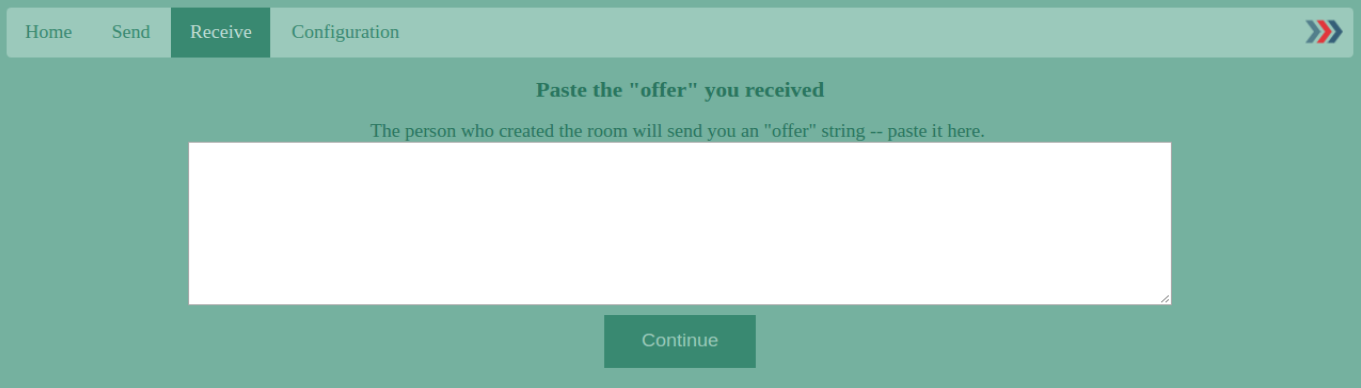
\includegraphics[width=\textwidth]{Figures/SL/receiver_offer}
  \decoRule
  \caption[Serverless mode: Input Offer screen]{This screen displays a white box where the user should paste the Offer received from the Sender. The continue button is only clickable after some information has been entered into the box.}
  \label{fig:serv_r_off}
\end{figure}
%	1. Input Offer \& senders mail
%		Box for pasting Offer and indicating who the sender is, for correct encryption and authentication. Click continue once the Offer is pasted. (Offer can be cleartext or cipher!)

%
\noindent
\underline{Third screen}
\begin{figure}[H]
  \centering
  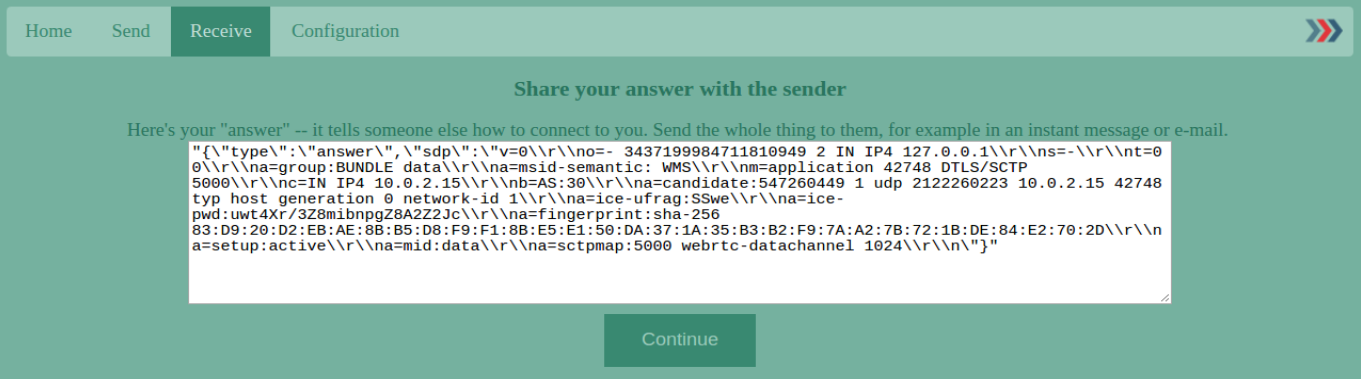
\includegraphics[width=\textwidth]{Figures/SL/answer}
  \decoRule
  \caption[Serverless mode: Display Answer screen]{This screen displays an empty white box until the Answer is generated. Once it is generated, it appears in the box along with a notification that it has been copied to the clipboard. The user should share this Answer with the Sender.}
  \label{fig:serv_r_ans}
\end{figure}
%	2. Show Answer
%		Shows box for displaying the Answer. After a short wait, the Answer will appear in the box, as well as automatically be copied to the clipboard. This can be either encrypted or cleartext, depending on if it is the first time communicating or not.

\subsubsection*{Shared:}
After the steps previously explained, the functionality and screens are the same for both the Sender and the Recipient. When these steps are completed, if no error or problems occur, it will follow the description given in \Cref{sec:file_recv}.
%

\subsection{Implementation specifics}
%
The biggest difference in implementation is of course the connection setup. Since the serverless solution has no set way of doing this, the connection setup will be discussed as part of the ACS mode, in \Cref{sec:acsimp}. In Serverless mode, the Offer and Answer is displayed in the form of a string. The string can either be a cipher or a cleartext representation of the Offer/Answer.

Since this part of SendIt has user interactions and relies on converting user input into JavaScript objects, it was at risk for XSS attacks and other code execution/injection attacks. As such, input sanitation was added to make sure that such attacks can not be executed. All data in this phase, both exported and imported, has to conform to the JSON format, which is then parsed and turned into JavaScript objects and used for establishing the connection via WebRTC.
%
\subsection{Possible improvements \& extendability}
%
This mode allows for no server-involvement, which in itself is a great way for companies to reduce expenses. For SendIt, it is only applied to file transfers via DataChannels. If this is applied to VOIP, which is currently one of the the most used applications of WebRTC, it could allow companies to increase profit margins. This does, however, set requirements for improving the lifetime of the connection setup. Specifically, the Answer will probably need to have it's lifetime doubled or tripled, for it to be usable in this scenario.

If one can somehow make changes to the current WebRTC system and make endpoints permanently addressable by a specific Offer and Answer combination, or allow the Offer and Answer to be re-usable, it would also benefit this solution a lot. Of course these permanent addressing or reusable Offers and Answers would have to be unique for each pairing, which might also raise some new issues. Working on extending the lifetime of the connection setup is objectively the best and most effective way to improve this solution.
%
%
\section{Assisted Connection Setup mode \textbf(ACS)}
%
%
Assisted Connection Setup mode alleviates some of the difficulties and problems from the Serverless mode, by automatically taking care of the connection setup. This is done through a server communicating by WS over HTTPS. It uses a custom protocol on top of WS, designed for sharing connection information for WebRTC, to control and understand the communication between the endpoints.

The server can be explicitly chosen by the users. They can host their own or choose to use an existing one offering this service. The only requirement is adhering to the pre-configured protocol. For details about the protocol, see \Cref{sec:wsprot} Because of this, the system is still unpredictable and hard to attack.

Another security feature is that there is no need for the server to send code to be executed or loaded by the client, as this functionality is pre-programmed in the client application. As such, the server has \emph{no influence} over the functionality of the client. The server only authenticates the user and forwards the connection information to the other endpoint.
In addition, all communication with the ACS happens over a secure channel, so an attacker would have to break the server itself to gain access to the information relayed. For more information about how the ACS server and the client communicates, see \Cref{sec:acsws}
%
\subsection{Use case}
%
The use case for this mode is when planning or co-ordinating with the other endpoint is not done in advance or hard to do. It is for when one is willing to sacrifice a small degree of security to improve the usability. This mode allows the connection request to be sent first, and only when the other endpoint has agreed to take part in the exchange, is the connection setup done. As such, the lifetime of the Offer and Answer is not an issue, since the exchange does not happen until both endpoints are online and ready to exchange information. It happens through an intermediary, so the exchange is almost instant. Since this intermediary is a point of attack and monitoring, it adds a small weakness to the system compared to the Serverless mode.
%
\subsection{Program flow}
%
The program flow is explained from after the functionality is chosen. For information about functionality other than Send and Receive, see the explanation in \Cref{sec:progflow}.
The ACS mode program flow differs depending on if the user has the role of Sender or Receiver. As such, the program flow of both of the roles will be shown and explained below.

Both roles begin with this screen, when entering ACS mode (This can be when starting the application, or when switching modes):
%
\begin{figure}[H]
  \centering
  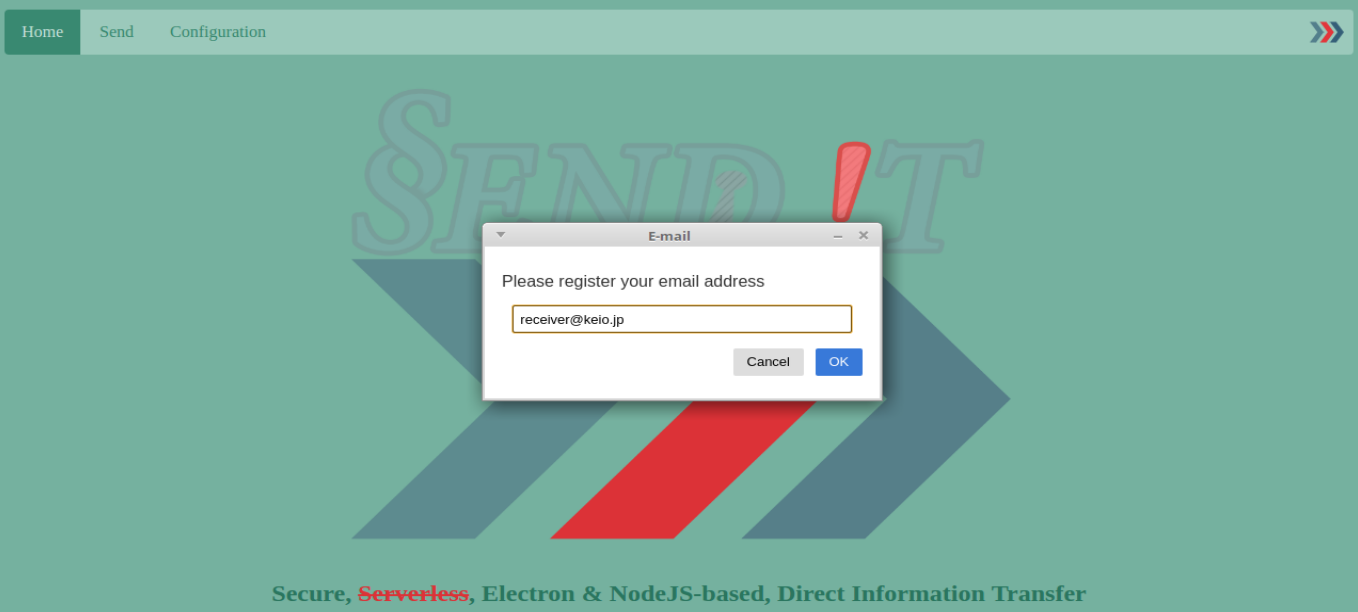
\includegraphics[width=\textwidth]{Figures/ACS/pop_up}
  \decoRule
  \caption[ACS mode: Identity selection screen]{The ACS mode requires an identity to be given, in order to be able to authenticate with the ACS server. This is also done so the ACS server knows where to forward data for each identity.}
  \label{fig:ACS_pop}
\end{figure}
%
\pagebreak
%
\subsubsection*{Sender:}
%
\noindent
\underline{First screen}
\begin{figure}[H]
  \centering
  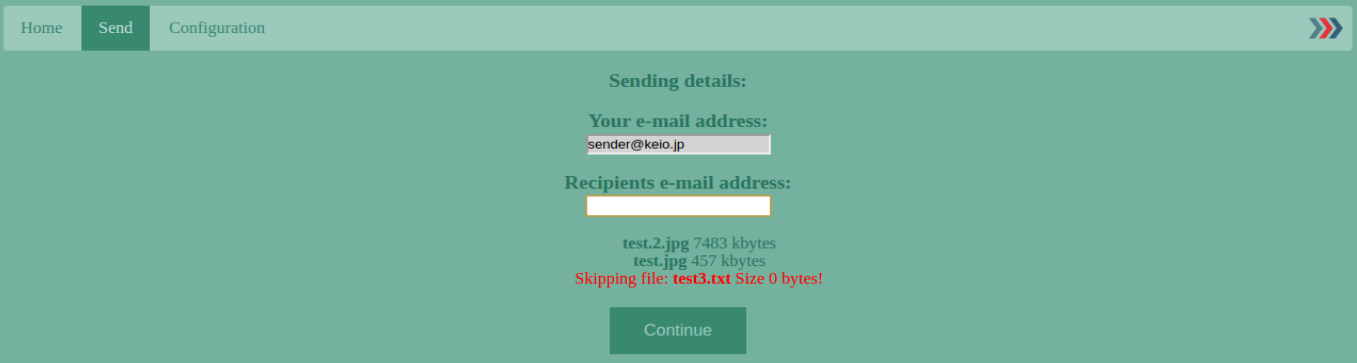
\includegraphics[width=\textwidth]{Figures/ACS/sending}
  \decoRule
  \caption[ACS mode: Sender screen]{This screen displays the e-mail address for the current identity, a field to indicate the Receivers e-mail address, and information about the file(s) to be transferred. If a file is marked in red, it means it will not be included.}
  \label{fig:ACS_send}
\end{figure}

\subsubsection*{Receiver:}
%
\noindent
\underline{First screen}\\
	It displays the e-mail for the current identity, the e-mail address of the intended Receiver (as indicated by the Sender), the Senders e-mail address, and data about the file(s). The user has two buttons: Accept and Decline. If the decline button is pressed, the user returns to the home screen.
\begin{figure}[H]
	\centering
	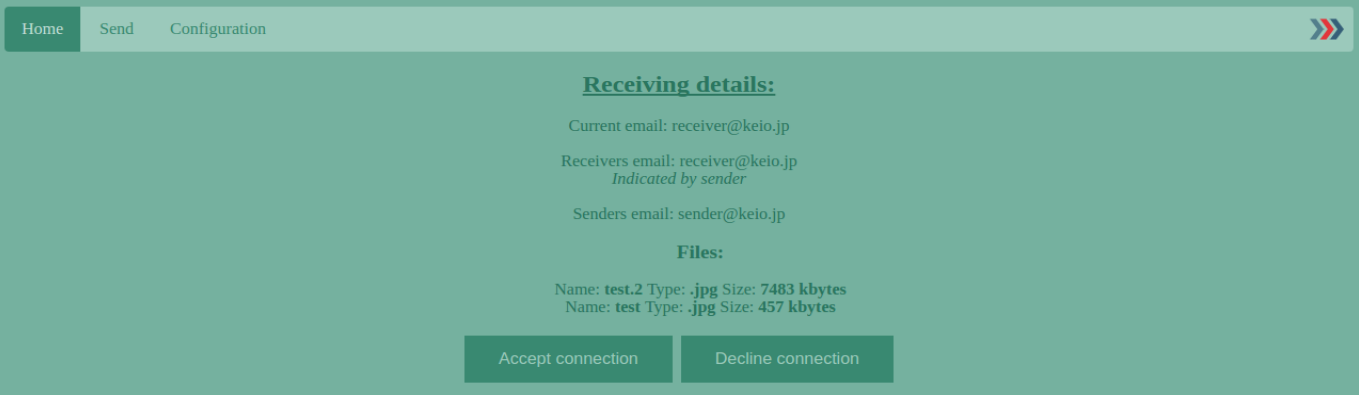
\includegraphics[width=\textwidth]{Figures/ACS/receiving}
	\decoRule
	\caption[ACS mode: Recipient screen]{This screen notifies the user that a connection request has been received and displays details about the Sender and the file(s) offered.}
  \label{fig:ACS_rec}
\end{figure}
%
\subsubsection*{Shared:}
After the previously explained steps are completed, if no error or problems occur, it will follow the description given in \Cref{sec:file_recv}. If an error occurs, a message will appear in the position shown in the next illustration, but on the screen currently being displayed.

\pagebreak
%
\noindent
\underline{Error screen}
\begin{figure}[H]
  \centering
  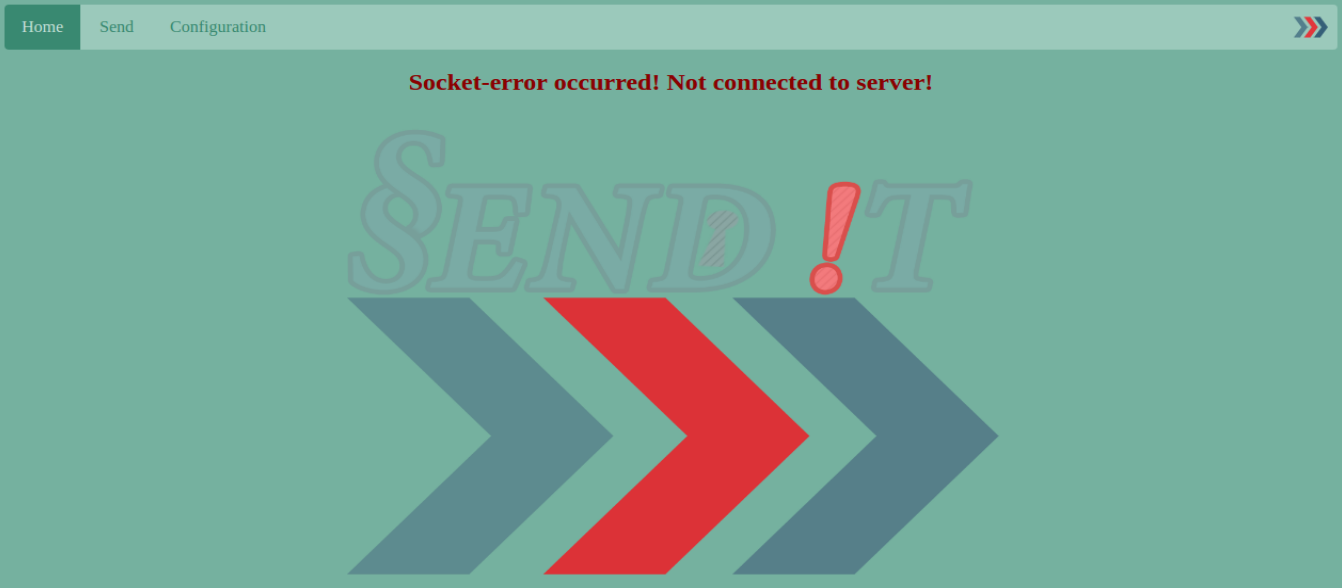
\includegraphics[width=\textwidth]{Figures/ACS/error}
  \decoRule
  \caption[ACS mode: Error screen]{This screen shows where the error will appear, if there is one. The message varies depending on which error occurs.}
  \label{fig:ACS_err}
\end{figure}

%
\subsection{Implementation specifics}
\label{sec:acsimp}
%
The biggest difference in implementation comes in the form of how the connection setup is exchanged and processed. The way of communicating with the ACS server and how the WebRTC connection setup is done, will be explained in this section. The functionality for actually sending the file(s) stays the same, but since the connection setup happens through a server, it needs a secure way to interact with the server. In this section the client-side implementation will be described. For more information about the server and the protocol used, please see \Cref{sec:acs_serv_des}. 
%
\subsubsection*{Communication:}
%
The ACS mode utilizes WebSockets to communicate with the server. It also forces the use of HTTPS to make sure that the communication is secure. All communication has to be in the format of the protocol described in \Cref{sec:wsprot}. This means that all information shared has to be processed and then correctly represented. Based on the information exchanged with the endpoint via the ACS, a P2P connection is established, just like in the Serverless mode. At this point the ACS server is no longer utilized. Once the connection has finished, for whatever reason, the ACS server is notified that the connection is over and that the endpoint is ready for a new connection.
%
\subsubsection*{WebRTC Connection setup:}
There are two major differences in how the connection setup for the P2P channel changes in this mode. First of all, the exchange does not just happen in the form of one Offer and one Answer. The method called ICE trickling, as described in \Cref{sec:webrtc_icetri}, is used. This separates the Offer and Answer from the ICE candidates. It allows for continuous exchange of ICE candidates, as well as a faster exchange of the Offer and Answer, since they can be shared without waiting for all the ICE candidates to be gathered before being shared. As such the lifetime of the Offer and Answer is irrelevant in this mode.

Secondly, the connection setup does not happen until both endpoints have agreed to connect to each other. This means that the endpoints are ready to receive and process the Offer and Answer, which allows the exchange to happen almost instantaneously. This minimizes the risk of any issues arising when doing the exchange and allows for an efficient connection setup. It also means that the endpoints do not redundantly create an Offer, thereby wasting time, in the case that the other endpoint declines the connection.

Finally, the roles of Sender and Receiver in SendIt, compared to in WebRTC, is reversed. This is to avoid the redundant creation of an Offer, as mentioned in the previous section. The Receiver in SendIt will receive a connection offer in the form of the screen showed in \Cref{fig:ACS_rec}. If the endpoint accepts this connection offer by pressing the accept-button, a WebRTC Offer will be generated and exchanged via the ACS server. Afterwards, functionality will be the same as in Serverless mode.
%
\subsection{Possible improvements \& extendability}
%
%REVIEW
Most of the improvements and extendability for this mode will rely on making changes to the current functionality of the ACS server. It would also require changes to the ACS client code, and as such, the discussion will be done in this section.

\subsubsection*{Key request:}
%Review
%REVIEW
Allowing the endpoints to request the key for an identity via the ACS server, would allow for encrypted end-to-end communication at all times. This requires some guarantee from the owner of the key to be attached, so the ACS server can not easily set up a MITM-attack. This would remove some of the issues with trusting the first exchange, and also allow for better trust evaluation and improved key exchange. The difficulty arises in the fact that the information needs to have a guarantee that it belongs to the correct identity, without having any previous or additional communication. One way to achieve this functionality is to go through the additional channel of using e-mail as a means of exchanging some shared secret, but this is left up to future work.
%
\subsubsection*{Multicast:}
%Review
Extending SendIt to allow \emph{false multicast} messages would mimic the way current e-mail attachments work and make sharing a file with multiple recipients at once easier. The reason for calling it \emph{false multicast} is because the transfer would still be one to one, but for the sender, it would seem identical to sending data to a multiple recipients. While this may allow for rapid spreading of malicious files, it would also improve usability in legitimate use cases. A way to achieve this is to have each client connect to a 'room' in the server, where the sender has to authenticate endpoints before/upon entering. After being authenticated, a P2P connection between the sender and the endpoint can be established and the file transferred.
%
\subsubsection*{Automatic reconnect:}
%Review
Automatically reconnecting after an endpoint has been disconnected or gone offline, would be a huge improvement to usability and user friendliness. It would allow for a very smooth user experience and increase the stability and reliability of the system. A way to achieve this would be to classify a connection as broken in the ACS server. This can be done by having endpoints report to the server if their connection is broken. The server then classifies the other endpoint as unavailable. Once the ACS server detects that the endpoint is once again available, it would automatically start the connection setup for both endpoints. The endpoints should have functionality that automatically accepts and connects, if this is the case.
%
\subsubsection*{Pausing connections:}
%Review
Allowing for pausing connections would increase user friendliness and help alleviate some issues that present when using synchronous communication. It would require some way to resume transfers from their previous point, but with such functionality in place, it should not be too hard to implement pausing connections. This would primarily be useful when being in the middle of a connection, when the need for transferring another file urgently occurs. Say the user is transferring a movie to a friend, when all of a sudden an important document from work needs to be received. Being able to temporarily pause the movie-transfer, receive the document, then resume the movie-transfer would be very useful. Having it automatically done through the ACS server, would be preferred.

% Chapter 6
%
\chapter{Conclusion} % Main chapter title
%
\label{Chapter6} % For referencing the chapter elsewhere, use \ref{Chapter6} 
%
This thesis has given an introduction to the current solutions available for file transfers and reviewed the advantages and pitfalls of these solutions. Afterwards, the basic technology and principles of SendIt were explained. Then the design and implementations specific to the base system were explained. After which it went through the specifics of each mode. Following, was a review of the experiments done and their contribution to the System, and an evaluation of SendIt and comparable systems. Finally, this chapter will summarize the work done and explore directions for future research.
%
\section{Summary}
%
This thesis has introduced a system and a prototype for improving the current situation of file transfers, focusing on e-mail attachments specifically. It did so by finding technology that fit well with the requirements and by developing an alternative solution. In an effort to return to the original idea behind the internet as a decentralized system, this thesis suggests a serverless system and shows a prototype of an implementation of such a system.

A serverless implementation also follows the logical idea of file transfers as a transaction only between two end-nodes. There is no reason to involve a third party unless absolutely necessary to do so. In addition, it also reduces the cost of running services, since central servers do not need to be hosted or managed. The disadvantage of such solutions is that there is no central management where one can access information easily or who can co-ordinate communication.
%
\paragraph{}
%
Since P2P technology allow us to avoid including a third party, this becomes the natural choice to use for the actual transfer of the files. While the usual way of creating P2P connections is by getting information from a server, or through DHT, SendIt suggests leaving it up to the users, since it will make the system more unpredictable while also allowing for easier use.

Since this creates additional burden on the user, the assisted connection setup mode was also developed. Endpoints send connection setup information to a server over secure WebSockets, which then relays it to the correct endpoint. While this does use a server, the server acts solely as a forwarding agent. Users can either use the default server, or host their own. An example of the default server is available with the code and installation files for SendIt. This is mainly to cater to the inexperienced users who cares more about usability than maximizing security. The opposite is true for the completely serverless version.

An added benefit, and another reason for choosing P2P communication was that it minimizes the attack surface of the application. Restricting the time of which the file or meta data about the file is available online greatly reduces the risk of an attacker gaining access to it.

The contrast from the proposed system compared to regular solutions is enormous considering the fact that files are usually left on servers even after the transfer has completed, which leave the information accessible for infinitely longer than with a direct solution. As such the suggested system is a clear improvement and has distinct advantages when it comes to reducing the attack surface of file-transfers. The drawback of P2P is also the inherit advantage. It is synchronous communication, which means that it is up to developers to find ways to facilitate asynchronous transfers by other means, if such functionality is wanted.
%
\paragraph{}
%
When choosing how to implement these features, WebRTC came forward as the logical option, because of its inherit support for many of the desired features. It offers serverless connection setup, creates P2P connections and also incorporates security functionality.  It offers authentication of peers based on the offer and answer and automatically encrypts the communications channel. It is also easy to deploy because it is a web technology, which means it can be used in an internet browser. That makes it easy to deploy and install.

There are two drawbacks of using WebRTC. The first is that it offers no consistent way to reach or address endpoint which means the connection setup has to be repeated every time a connection is to be made. The second is that there is also no way to consistently identify or authenticate users. For the first issue, there are no easy remedies, the second can be solved by adding an additional identification and authentication scheme.
%
\paragraph{}
%
For such a scheme, there are many options available. The most used one in public key cryptography, and for good reason. As outlined in \Cref{sec:pkc}, it is a system for encryption and decryption that ensures confidentiality and integrity, while also being easy to manage. By associating each identity with a public key, we can easily ensure that only the entity with the corresponding private key can access the information. This protects users privacy as well as make sure that it is not possible for attackers to see or manipulate the contents of the data.

The downside of public key cryptography is that it is hard to understand and manage correctly by people who are less technically capable. They have a hard time understanding the concept behind how it works, the difference between the two keys, and how to utilize it in practice. In the proposed system, this is taken care of programmatically and the users do not have to worry about such issues.

In order for the encryption and decryption to be useful, we have to make sure that we are using the correct key when communicating with a user. That is where identity management and trust comes in to the picture. To be able to use public key cryptography you need to exchange keys, and only then can you encrypt data.

The exchange of keys is usually done through a trusted third party, in the form of a server. Since SendIt does not have a central server to rely on, the first connection and with it the exchange of keys, is regarded as a trusted connection. What this means is that we assume the information is correct and not being supplied by a malicious user. Afterwards the system can guarantee all the benefits of public key cryptography, but it relies on this first setup being correct. In order to reduce the risk of an attacker exploiting this, a trust system is suggested.

The web of trust model allows users to re-evaluate and nuance our trust in endpoints. This gives a collective view of who is trustable and who is not, and can also help detect attackers trying to abuse the first trust. While this initial trust is detrimental to the security of the system, changing it would affect usability severely. As such the system is built upon this first trust, with the web of trust model as a continuous evaluation to detect attackers and minimize the effect of potential attackers. It is possible to extend or change this functionality, if one so pleases, when using SendIt as a platform for further development.
%
\paragraph{}
%
These features creates the basis for a reasonably secure system. In addition, the system is made to be as user friendly as possible. Installation is extremely easy as all that is required is downloading the installer and executing it. There are no options or dialogs during the installation. There is also no requirement to sign up, to do any key management, or any other aspects that may take focus away from the main goal: transferring files.

The user only has to care about placing the files in the correct folder and initiating the transfer to the correct destination. In a similar fashion, when receiving files, all one has to do decide is accept or decline such an offer. The functionality is clear and easy to use. The flow of the program is easy to follow and requires little interaction from the user.

Once the transfer is complete, the connection is automatically torn down and the user can start a new transfer. All of these features is to make sure that people with low technical understanding can still get the benefit of using the system. The difficult technical parts are automatically set up and taken care of for the user. Advanced users are also kept in mind, however, as they are allowed access to details and can make changes in settings window.
%
\paragraph{}
%
Comparing SendIt to existing solutions clearly illustrates the advantage of direct communication and the increase this yields in regards to protecting users security and privacy. It gives the user better control over where their data is, and also reduces the chance that an attacker can gain access to the data.

Additionally, it requires no setup on the user side and can be used directly after installation has finished. While other solutions have encryption and authentication, the systems are not clear to the user and they can easily be tricked by false E2E encryption. This is not the case for SendIt as it can be easily inspected and managed. One can also easily switch identities if desired, without any issues or having to do a lot of setup, unlike the comparative solutions.
%
\paragraph{}
%
The contributions of this thesis can be summed up as a user-friendly system that allows for direct, secure file transfers. SendIt can also serve as a platform to expand for a wide range of functionality and services. SendIt as a platform would like be used for its identity management and authentication functionality, not the file transfer functionality. While this is one use case, another can be adding more functionality to the file transfer aspect, as it would allow it to become more of a complete solution that could function as a stand alone system, instead of a complimentary one.

It also contributes to exploring new implementations of e-mail attachments. The serverless functionality also opens for a new way of software developing, and contributes and encourages a break with the current server-based development. Finally, it shows that secure solutions do not necessarily have to be hard to use and incentivizes development of more user-friendly security applications.
%
\paragraph{}
%
In conclusion: This thesis introduced a system that improves the current implementation of e-mail attachments. It does so by directly transferring files, lowering the attack surface significantly. It also guarantees end-to-end encryption and endpoint authentication, which is not commonly used in e-mail attachments, making it resistant to both active and passive attacks. It achieves this while keeping the system easy to use to doing key-management and authentication on behalf of the user, without the need for any setup or central corraboration. SendIt outperforms e-mail attachments in regard to security, as well as usability and cost efficiency.The drawback of SendIt is the limitation of only supporting synchronous transfers as well as its inherent trust in the first connection.
%
\section{Future work}
%
There are still many venues and ways of improvement for systems such as SendIt, and e-mail attachments in general. By separating future works in to two sections, it is easier to get a clear view of which improvements are necessary for SendIt, and which are more for e-mail attachments in general.

SendIt has the core features and design developed, but since it has been a one person job, the depth and complexity has been limited. With more time or more manpower, a lot of the issues currently existing can be fixed and a complete replacement to the current e-mail attachments can be completed. As such the future research for SendIt focuses more on implementations and testing of the system.

For e-mail attachments in general, a more holistic approach is taken in regards to future work. Things like large scale evaluation and system design becomes more important and needs to be prioritized and given a greater importance than when designing a simpler system.
%
\subsection{SendIt}
%
The following topics can be future research for the development for SendIt:
\begin{itemize}
	\item Developing and testing extendability of the connection setup for the serverless mode. Adding to the lifetime of the connection setup would greatly increase the usability and reliability of this mode. Adding some kind of connection-manager or middleware, was considered as part of this research, but could not be done in time.
	\item Improving reliability of connections and connection setup. In the same vain as the point above, increasing the success rate of the connection setup would make the system more reliable and easier to use. Making sure connections are stable and do not disconnect also helps the usability and stability of the system.
	\item Exploring more ways to evaluate trust. Testing, implementing and comparing different systems in practice, as well as finding an algorithm for evaluation. This work would add great value to the trust management of SendIt.
	\item Improve the initial trust. Finding a way to increase the trust in the first connection or some way of authentication that does not rely on a central service would be a big improvement. In addition, allowing for sharing keys across applications may also be a way to bridge this initial trust issue. Such problems are left up to future research.
	\item Adding support for pausing transfers. Having a way to pause transfers should be easy to implement, and will benefit the system greatly. Especially for big transfers, this will allow users to take breaks temporarily, if needed.
	\item Checking overhead of file-transfer and optimizing the protocol. Making sure and optimizing the speed of the file transfer can be useful for having as effective communication as possible. This would allow for shorter transfer-times, less data transferred and higher efficiency.
	%\item Finalize protocol and ACS server. Completing this work will add extra trust to the system and help make the key-exchange go smoothly. While this is not critical to the system in any way, it would make for an increase in security and improve the trust in an identity.
\end{itemize}
%
\subsection{E-mail attachments}
%
The following topics can be future research for e-mail attachments and how to improve the current system:
\begin{itemize}
	\item Finding a better way to asynchronously transfer files. Any improvement to the way e-mail attachments currently work would be a welcome contribution, but particularly an improvement to user privacy is necessary. Avoiding server-storage would be optimal, but finding a way to ensure that the file does not reside on the server after the message has been transferred, would also be good.
	\item Exploring other systems and alternatives to SendIt. Evaluating their usability and functionality. By doing this work, one can clearly indicate which solution is optimal and recommend a new standard which can be adopted by e-mail clients.
		\item Creating alternative solutions to complement SendIt. As mentioned in the introduction (\Cref{Chapter1}), replacing the current email attachment system with SendIt alone is not recommended. Developing a complementary system to SendIt, which in combination can be implemented to completely replace the current system would go a long way towards changing the current ecosystem.
\end{itemize}
%
\section{Final remarks}
%
As a final note, I would like to add that the source code for both SendIt and the ACS server will be made available \href{https://github.com/Robiq}{on github}\footnote{\href{https://github.com/Robiq}{https://github.com/Robiq}} once it has been cleared for release. I hope it will be developed further and that it can succeed as an open source application.
\chapter{System evaluation} % Main chapter title
%
\label{Chapter7} % For referencing the chapter elsewhere, use \ref{Chapter7} 
%
To understand the contribution and usability of SendIt, an analysis of existing solutions is needed. By comparing SendIt with existing solutions it is possible to get an idea of what has been improved, what stayed the same, and what still needs to be improved. In the following section the e-mail system, a generic SNS system and SendIt will all be evaluated and analyzed.

 It will also discuss and compare SendIt to other solutions, and evaluate how SendIt matches up against these solutions.
%
\section{Evaluation of SendIt}
%
  SendIt has fewer weaknesses than the other two systems. The main advantage is the direct transfer, which minimizes the attack surface compared to the other two solutions. This evaluation will not include all attacks made possible by the technology chosen, but rather focus on the weaknesses that come as a consequence of the proposed system. By this it is meant that attacks that are present in all JavaScript solutions will not be discussed. If the attack is possible because of the way JavaScript is used in this solution, it will be included.
%
  %First trust!!!
  \subsection{First trust}
  %
  The main weakness, as mentioned previously, is the first trust. This can allow an attacker to appear as the legitimate owner of an identity, without this being the case. This is a risk that any user should be aware of, as it is a critical part of the system. Even though it is a part of the design choice, it has to be acknowledged that this is less than optimal.

  The mitigation for such attacks is split in two parts. The first is relying on the user to evaluate whether the user is legitimate. By using social cues like timing, each user should evaluate if it is likely that the other identity would initiate a transfer. One can also contact the other endpoint and confirm that it is actually them. This is, of course, only necessary for the first connection.

  The second is the trust model, which is an automatic part of the system. It combats this issue by sharing information and allowing users to have as much data as possible, for all identities. This allows for detection of false identities and will eventually make these identities untrusted entities in the whole system.
%
  \subsection{DHT}
  While P2P transfer is direct communication between two endpoints, it needs some way to set up the connection. Traditionally this has been done using servers or DHT networks. Since the whole point is to avoid using servers, the only option left is DHT. DHT solutions rely on connecting to specific endpoints, called bootstrapping, to enter the network. This is predictable behavior that can be exploited by attackers, and it also increases the difficulty of using the system.

  As such, the system suggested in this thesis leaves it up to the end users to decide how to share the information, as it is unpredictable and allows for easier usage of the system. It removes the need for any bootstrapping or server, and does not specify any set way to share the connection information.
  
  %ACS!!!
  \subsection{ACS}
  %
  Another attack vector is the ACS server. If it is not trusted, it can pose a security risk, as the endpoint has to rely on the fact that the ACS server relays the data to the correct recipient. If the data sent is encrypted, it will not pose any immediate risk, but it will stop the endpoint from connecting to anyone, as the other endpoint will not get authenticated properly. If it is the first time these endpoints are connecting, however, it puts the victim at risk of being put in touch with the wrong identity.

  The ACS server can also act as a logger that keeps track of which identities are communicating with each other. While not directly an attack, it can raise privacy issues, since it allows for monitoring of traffic. It can also be argued that it can be used for reconnaissance, which allows for a targeted attack on one of the endpoints. Because of this, endpoints should only use ACS servers they trust.

  %MITM
  The ACS server can also deploy MITM-attacks during the connection setup, which leads to the attacker gaining full access to the data transferred. The biggest problem with this type of attack is that, in most cases, it cannot be detected until after the data has already been shared and the attacker has full access to it. It will eventually be detected by the trust system, but at that point it might already be too late. While there is also a possibility for this to happen during the connection setup of the Serverless mode, it is much harder to do, since there is no pre-determined channel for sharing the Offer/Answer, and as such, the attacker has no set point to attack. 
%
  %XSS
  \subsection{Other}
  Finally, there is a theoretical possibility of having XSS attacks executed in the client, since the Serverless mode relies on user input. While there are countermeasures deployed, one can never guarantee that there are no such security holes.

%
%
\section{E-mail system comparison}
\label{sec:email_syst}
  %E-mail
  %Anything is an improvement
  Comparing the e-mail system to SendIt is a little like comparing your mailbox to a safe. While the mailbox can be locked and it can be made more secure, it is still outside your house, with no access control, not made to withstand attacks, and ultimately, it can just be stolen as a whole. In contrast, the safe is made to withstand attacks, and store your data privately.

  In a similar fashion, e-mail was made to send and receive information, like a mailbox. SendIt is made to make this process secure against outside tampering and allow for minimal risk while exchanging information. To continue the analogy, it is like meeting the Sender with your safe, giving the Sender a small slot to put the mail in, that only fits the letter you expect to receive, and immediately returning back to the safety of your house. SendIt would be the safe in the aforementioned scenario. To summarize, the email system offers some secure solutions, but guarantees none. In practice, that means one should assume that none is applied. Therefore, anything is an improvement.
%
%
  \subsection{Direct transfer}
  \label{sec:ev_dir}
  %No temporary storage - direct transfer
  The first major advantage SendIt has over traditional e-mails, is that it transfers the file directly. None of the issues stemming from files being stored in transit applies to SendIt. These issues range from attackers hacking the server and getting access to the files, to allowing attackers to monitor data going through the server, since the data will always pass through this point. As a general rule, a resource is more secure, the fewer copies exist, since it limits the attack surface.

  %Files will be broken if given enough time
  Another point to take into consideration is that even if only encrypted data is stored on a server, if an attacker gets access to the data, it is only a question of how long it takes to break the encryption. As such, minimizing the risk of leaking any data should be considered critical. This is why direct transfer of files offer such an advantage.

  %Lower attack surface - direct transfer (TIME!)
  The attack surface which is exposed is also important to evaluate. Having a server store the files, means the attack surface is quite large, since it is always online. With SendIt's direct transfer function, the file is only available during transfer. The time difference for how long the file is available to be attacked is huge. As such, this is another advantage of direct transfer, since the attack surface is significantly reduced.
%
  \subsection{Authentication}
  %No possibility to impersonate real Sender
  Sender and Receiver guarantee is another advantage of SendIt. In the e-mail system, the Sender's identity can be forged easily, which is not the case for SendIt. It also has some issues where the data sent is not kept confidential and can easily be stolen by a passive listening attack. These two combined make phishing attacks, as well as targeted exploits, easier to create, since you know what data or information the endpoint is seeking or expecting. By sending this data from a forged address, the chances of successful attacks increase. The e-mail system has S/MIME which allows for authentication, but as discussed in \Cref{sec:intro_email}, it is rarely used and is not user friendly.
  %
  \subsection{Content control}
  %All content received
  In the ordinary e-mail system, one is also not able to stop unwanted content. If someone sends an e-mail attachment, it will be delivered to the receiver's PC, or at least their e-mail server. This is unfortunate, since receiving malicious files may cause them to be executed at a later time, or by an unintended action. It is also possible that they may execute without the user knowingly doing so. As such, it is optimal for the user to be able to stop the transfer of unwanted files, something which SendIt supports.
  %Automated spreading
  Automatic spreading of malicious files is a big problem today. It is spread to all the victim's contacts and keeps spreading in a similar fashion. While SendIt has no direct solution to mitigate this, the fact that it does not support multicast, and that the files cannot be automatically received, will naturally take care of resolving this issue.
%
%
  \subsection{Connection setup}
  \label{sec:ev_con}
  % - Needs connection setup
  The disadvantage of SendIt is that it is required to complete a connection setup phase in order to communicate with the other endpoint. The e-mail system has no such need and one can easily transfer information at any time without the user having to worry about the connection setup. This is because all communication occurs between the client and a server that is publicly available.
%
  \subsection{Synchronous connection}
  % - Synchronous
  Another case where SendIt exhibits different behavior is during the actual transfer. While the advantages of direct transfers have been clearly indicated, SendIt does lack support for asynchronous transfers. This is a point where the regular e-mail solution has the edge over SendIt. It can be argued, however, that it is a small obstacle to overcome, for such an increase in security.
%
  \subsection{First trust}
  \label{sec:ev_first}
  % - First trust
  Finally, the e-mail system does not have to rely on the trusted first setup, that SendIt does. In the case that the e-mail system uses the security features available, it relies on PKI for the initial trust. This choice of a central service makes sense in the e-mail system which relies on servers, but not for SendIt.
%
  %
\section{SNS and Cloud systems comparison}
  %SNS
  While there is no one SNS or cloud based system to compare against, they all share certain functionality and design choices. As such, this generalization will be the model used for comparison. As discussed in \Cref{sec:ev_dir}, SendIt directly transfers the file, removing the need for central storage, thereby lowering the attack surface. While the original point is made in comparison to the e-mail system, this applies equally to SNS and Cloud based systems. This is why SendIt provides a clear use case and improvement to current systems.
  %No temporary storage - direct transfer
  %Files will be broken if given enough time
  %Lower attack surface - direct transfer (TIME!)
%
  \subsection{False E2E encryption}
  %'E2E encryption' not real - skype!
  As mentioned in \Cref{sec:cloudetc} and shown in \Cref{fig:sns}, false E2E encryption is sometimes utilized in these systems. This is a scary thing, as a consumer of these services, because both you and your communication partner are unable to verify if the communication has true E2E encryption or not. Effectively, this is a MITM-attack by design. As such, when using these services, one should assume that the data can be decrypted and read by the service and whoever they disclose the data to. For SendIt, the public-key cryptography guarantees end-to-end encryption, since the keys are exchanged over P2P, which means no central service can tamper with the keys sent. 
%
  \subsection{Identity swapping}
  %Hard to switch identities
  Another thing that is hard to do in these systems is swap identities, if the user desires. One may not want to associate an identity with both work and private life, which means the need for several identities arises. This requires logging in and out, managing two sets of credentials, and keeping track of which identity is currently in use. For SendIt, all the user has to do is swap to the file containing the correct keys and the identity has been changed.
%
  \subsection{Other}
  The points where SNS and Cloud based systems have clear advantages also resembles that of the e-mail system. The points made in \Cref{sec:ev_con} and \Cref{sec:ev_first} apply to these systems as well. For the first trust in these systems, they also rely on the PKI model, which is understandable, since they are also based around the server-client model.

  These solutions do have the advantage of storing a backup of your files, which can be desired in certain situations. Though this can easily be done after the transfer has completed, which gives the user more control over how it is stored. As such, these solutions are more suited for regular files, not files with high requirements in regard to privacy and security.
  % - Needs connection setup
  % - First trust
% Chapter 8
%
\chapter{Conclusion} % Main chapter title
%
\label{Chapter8} % For referencing the chapter elsewhere, use \ref{Chapter8} 
% REDO WHEN UPDATING 
This thesis has given an introduction to the current solutions available for file transfers, and reviewed the advantages and pitfalls of these solutions. Afterwards, the basic technology and principles of SendIt were explained. Then the general design and implementations were explained. After which it went through the specifics of each mode. Following, was a review of the experiments done and their contributions to the system, and an evaluation of SendIt and comparable systems. Finally, this chapter will summarize the work done and explore directions for future research.
%
\section{Summary}
%
This thesis has introduced a system and a prototype for improving the current situation of file transfers, focusing on e-mail attachments specifically. It did so by finding technology that fit well with the requirements, and by developing an alternative solution. In an effort to return to the original idea behind the Internet as a decentralized system, this thesis suggests a serverless system and shows a prototype of an implementation of such a system.

A serverless implementation also follows the logical idea of file transfers as a transaction only between two end-nodes. There is no reason to involve a third party, unless absolutely necessary. In addition, it also reduces the cost of running services, since central servers do not need to be hosted or managed. The disadvantages of a serverless implementation is that there is no central management where one can access information easily, nor a central entity who can co-ordinate communication.
%
\paragraph{}
%
Since P2P technology allows us to avoid including a third party, this becomes the natural choice to use for the actual transfer of the files. While the usual way of creating P2P connections is by getting information from a server, or through DHT, SendIt suggests leaving it up to the users, since it will make the system more unpredictable, and as such harder to attack, while also allowing for easier use.

Since this creates additional burden on the user, the Assisted Connection Setup mode was also developed. Endpoints send connection setup information to a server over secure WebSockets, which then relays it to the correct endpoint. While this does use a server, the server acts solely as a forwarding agent. Users can either use the default server, or host their own. An example of the default server will be available with the code and installation files for SendIt. This is mainly to cater to the inexperienced users who care more about usability than maximizing security. The opposite is true for the completely serverless version.

An added benefit, and another reason for choosing P2P communication, was that it minimizes the attack surface of the application. Restricting the time of which the file, or metadata about the file, is available online greatly reduces the risk of an attacker gaining access to it.

The contrast from the proposed system compared to regular solutions is enormous considering the fact that files are usually left on servers even after the transfer has completed, which leaves the information accessible for infinitely longer than with a direct solution. As such, the suggested system is a clear improvement, and has distinct advantages when it comes to reducing the attack surface of file transfers. The drawback of P2P is also the inherent advantage: It is synchronous communication. This means that it is up to developers to find ways to facilitate asynchronous transfers by other means, if such functionality is wanted.
%
\paragraph{}
%
When choosing how to implement these features, WebRTC came forward as the logical option, because of its inherent support for many of the desired features. It offers serverless connection setup, creates P2P connections, and also incorporates security functionality.  It offers authentication of peers, based on the Offer and Answer, and automatically encrypts the communications channel. It is also easy to deploy because it is a web technology, which means it can be used in an internet browser, making it easy to deploy and install.

There are two drawbacks of using WebRTC. The first is that it offers no consistent way to reach or address endpoints, which means the connection setup has to be repeated every time a connection is to be made. The second is that there is no way to consistently identify or authenticate users. For the first issue, there are no easy remedies, the second can be solved by adding an additional identification and authentication scheme.
%
\paragraph{}
%
For such schemes, there are many options available. The most used scheme is public-key cryptography, and for good reason. As outlined in \Cref{sec:pkc}, it is a system for encryption and decryption that ensures confidentiality and integrity, while also being easy to manage. By associating each identity with a public key, the system guarantees that only the entity with the corresponding private key can access the information. This protects user privacy, as well as, making sure that it is not possible for attackers to see or manipulate the contents of the data.

The downside of public-key cryptography is that it is hard to understand and manage correctly by people who are less technically capable. They have a hard time understanding the concept behind how it works, the difference between the two keys, and how to utilize it in practice. In the proposed system, this is taken care of programmatically and the users do not have to worry about such issues.

It is important to use the correct key for the corresponding endpoint, in order for the encryption and decryption scheme to be useful. This is why identity management and trust is necessary. To be able to use public-key cryptography, users need to exchange keys and, only then, can data be encrypted.

The exchange of keys is usually done through a trusted third party, in the form of a server. Since SendIt does not have a central server to rely on, the first connection, and with it the exchange of keys, is regarded as a trusted interaction. What this means is that the system assumes the information is correct and not being supplied by a malicious user. Afterwards, the system can guarantee all the benefits of public-key cryptography, but it relies on this first setup being correct. In order to reduce the risk of an attacker exploiting this, a trust system is suggested.

The web of trust model allows users to re-evaluate and nuance their trust in endpoints. This gives a collective view of who is trustworthy and who is not, and can also help detect attackers trying to abuse the first trust. While this initial trust is detrimental to the security of the system, changing it would affect usability severely. As such, the system is built upon this first trust, with the web of trust model as a continuous evaluation to detect attackers, and to minimize the effect of potential attackers. It is possible to extend or change this functionality, if one so pleases, when using SendIt as a platform for further development.
%
\paragraph{}
%
These features create the basis for a reasonably secure system. In addition, the system is made to be as user friendly as possible. Installation is extremely easy, all that is required is downloading the installer and executing it. There are no options or dialogs during the installation. There is also no requirement to sign up, to do any key management, or any other aspects that may take focus away from the main goal: transferring files.

The user only has to care about placing the files in the correct folder and initiating the transfer to the correct destination. In a similar fashion, when receiving files, all one has to do is decide whether to accept or decline such an offer. The functionality is clear and easy to use. The flow of the program is easy to follow, and requires little interaction from the user.

Once the transfer is complete, the connection is automatically torn down and the user can start a new transfer. All of these features are there to make sure that people with low technical understanding can still get the benefit of using the system. The difficult, technical parts are automatically set up and taken care of for the user. Advanced users are also kept in mind, as they are allowed access to details about the system and can make changes in the settings window.
%
\paragraph{}
%
Comparing SendIt to existing solutions clearly illustrates the advantage of direct communication and the increase this yields in regards to protecting users security and privacy. It gives the user better control over where their data is, and also reduces the chance of an attacker gaining access to the data.

Additionally, it requires no setup on the user side, and can be used directly after installation has finished. While other solutions have encryption and authentication, the systems used cannot be inspected by the user, and they can easily be tricked by false E2E encryption. This is not the case for SendIt as it can be easily inspected and managed. One can also easily switch identities, if desired, without having to create a new account or go through additional steps. This is in stark contrast to the comparative solutions.
%
\paragraph{}
%
The contributions of this thesis can be summed up as a user-friendly system that allows for direct, secure file transfers. SendIt can also serve as a platform to expand for a wide range of functionality and services. SendIt, as a platform, would likely be used for it's identity management and authentication functionality, not the file transfer functionality. While this is one potential use case, another can be adding more functionality to the file transfer aspect. This would allow it to become more of a complete solution that could function as a stand alone system, instead of a complimentary one.

It also contributes to exploring new implementations of e-mail attachments. The serverless functionality also opens for a new way of software developing, and contributes and encourages a break with the current server-based development. Finally, it shows that secure solutions do not necessarily have to be hard to use and incentivizes development of more user-friendly security applications.
%
\paragraph{}
%
\textbf{In conclusion:} This thesis introduced a system that improves the current implementation of e-mail attachments. It does so by directly transferring files, lowering the attack surface significantly. It also guarantees end-to-end encryption and endpoint authentication (\emph{based on the key exchange done as part of the first connection}), which is not commonly used for e-mail attachments, making it resistant to both active and passive attacks. It achieves this while keeping the system easy to use, by taking care of key management and authentication on behalf of the user, without the need for any setup or central corroboration. SendIt outperforms e-mail attachments in regards to security, as well as usability, and cost efficiency. The drawbacks of SendIt are the limitation of only supporting synchronous transfers, as well as, it's inherent trust in the first connection.
%
\section{Future work}
%
There are still many venues and ways of improvement for systems such as SendIt, and e-mail attachments in general. By separating future work into two sections, it is easier to get a clear view of which improvements are necessary for SendIt, and what changes are needed in regards to e-mail attachments in general.

SendIt has the core features and design developed, but since it has been a one person job, the depth and complexity has been limited. With more time or more manpower, many of the issues currently existing can be fixed, and a complete alternative to the current e-mail attachment functionality can be finalized. As such, the future research for SendIt focuses more on implementations and testing of the system.

For e-mail attachments in general, a more holistic approach is taken in regards to future work. Things like large scale evaluation and system design become more important and need to be prioritized more than when designing a simpler system.
%
\subsection{SendIt}
%
The following topics can be future research for the development for SendIt:
\begin{itemize}
	\item \textbf{Developing and testing extendability of the connection setup for the Serverless mode.} Adding to the lifetime of the connection setup would greatly increase the usability and reliability of this mode. Adding some kind of connection-manager or middleware was considered as part of this research, but could not be done in time.
	%
	\item \textbf{Improving reliability of connections and connection setup.} In conjunction with the point above, increasing the success rate of the connection setup would make the system more reliable and easier to use. Making sure connections are stable and do not disconnect will help the usability and stability of the system.
	%
	\item \textbf{Exploring more ways to evaluate trust.} Testing, implementing, and comparing different systems in practice, as well as finding an algorithm for evaluation. This work would add great value to the trust management of SendIt.
	%
	\item \textbf{Improve the initial trust.} Finding a way to increase the trust in the first connection, or some way of authentication that does not rely on a central service, would be a big improvement. In addition, allowing for sharing keys across applications may also be a way to bridge this initial trust issue. Such problems are left up to future research.
	%
	\item \textbf{Adding support for pausing transfers.} Having a way to pause transfers should be easy to implement, and will benefit the system greatly. Especially for big transfers, this will allow users to take breaks temporarily, if needed.
	%
	\item \textbf{Checking overhead of the file transfer and optimizing the protocol.} Optimizing the speed of the file transfer, as well as, minimizing the overhead of the protocol, will ensure that the communication is as effective as possible. This would allow for shorter transfer-times, less data transferred, and higher efficiency.
	%
	%\item Finalize protocol and ACS server. Completing this work will add extra trust to the system and help make the key exchange go smoothly. While this is not critical to the system in any way, it would make for an increase in security and improve the trust in an identity.
\end{itemize}
%
\subsection{E-mail attachments}
%
The following topics can be future research for e-mail attachments and how to improve the current system:
\begin{itemize}
	\item \textbf{Finding a better way to asynchronously transfer files.} Any improvement to the way e-mail attachments currently work would be a welcome contribution, but particularly an improvement to user privacy is necessary. Avoiding server-storage would be optimal, but finding a way to ensure that the file does not reside on the server after the message has been transferred would be an acceptable compromise.
	%
	\item \textbf{Exploring other systems and alternatives to SendIt.} Evaluating their usability and functionality. By doing this, one can clearly indicate which solution is optimal, and recommend a new standard which can be adopted by e-mail clients.
	%
	\item \textbf{Creating alternative solutions to complement SendIt.} As mentioned in the introduction (\Cref{Chapter1}), replacing the current email attachment system with SendIt alone is not recommended. Developing a complementary system to SendIt, which in combination can be implemented to completely replace the current system, would go a long way towards improving the current situation.
\end{itemize}
%
\section{Final remarks}
%
As a final note, I would like to add that the source code for both SendIt and the ACS server will be made available \href{https://github.com/Robiq}{on github}\footnote{\href{https://github.com/Robiq}{https://github.com/Robiq}} once it has been cleared for release. I hope it will be developed further, and that it can succeed as an open source application that provides improved security and privacy for everyone.

%----------------------------------------------------------------------------------------
%	THESIS CONTENT - APPENDICES
%----------------------------------------------------------------------------------------

\appendix % Cue to tell LaTeX that the following "chapters" are Appendices

% Include the appendices of the thesis as separate files from the Appendices folder
% Uncomment the lines as you write the Appendices

% Appendix Template

\chapter{ACS Server} % Main appendix title

\label{AppendixA} % Change X to a consecutive letter; for referencing this appendix elsewhere, use \ref{AppendixX}

\begin{lstlisting}[caption=ACS Server, style=htmlcssjs]
const HTTPS_PORT = 7443;

const fs = require('fs');
const https = require('https');
const WebSocket = require('ws');
const WebSocketServer = WebSocket.Server;
const q = require('./resources/queue.js');
const crypto = require('@trust/webcrypto');
var uuid=1;
var sockuuid=1;
var sUUID = 0;
var conn = {};
var key = new Object();

var wss_prot = {
//Authentication	
	AUTH_SETUP: "setup", //Register keys
	AUTH_S_REPLY: "setup_reply", //Registration OK/NOT OK
	AUTH_INIT: "auth_init", //Start authentication
	AUTH_RESULT: "result", //Authentication result

//All directions
	ERROR: "error", //error occured - specified in data
	WAIT: "wait", //Waiting for other end - specified in data

//Client-Server messages
	INIT: "start", //Offer sending - forwarded
	DONE: "done", //Connection finished
	REQKEY: "request_key", //Request public key - Include own public key!

//Server-Client messages
	KEY: "key", //Share keys for other end

//Client-Client messages
	ACCEPT: "accept", //Accept offer - contains offer!
	REFUSE: "refuse", //Refuse offer
	ANSWER: "answer", //Contains answer
	ICE: "ice", //Contains ICE-candidates
	LOOKUP: "lookup" //For looking up email presence
};

//console.log("Argv1: " + process.argv[2]);

// Yes, SSL is required
const serverConfig = {
    key: fs.readFileSync('server-key.pem'),
    cert: fs.readFileSync('server-cert.pem'),
};

start();

// Create a server for the client html page
var handleRequest = function(request, response) {
    // Render the single client html file for any request the HTTP server receives
    console.log('request received(https): ' + request.url);
    try{
    	//If testing, serve files
    	if (process.argv[2] === 'test'){
	    	if(request.url === '/') {
	            response.writeHead(200, {'Content-Type': 'text/html'});
		        response.end(fs.readFileSync('/home/robin/Project/Server/test/wss_test.html'));
	        } else if(request.url === '/wss_test.js') {
		    	response.writeHead(200, {'Content-Type': 'application/javascript'});
		        response.end(fs.readFileSync('/home/robin/Project/Server/test/wss_test.js'));
		    }else{
	        	console.log('Invalid URL requested - no HTML support!');
		        response.writeHead(404);
		        response.end();
		    }
		//If production no files!
		}else{
			console.log('Invalid URL requested - no HTML support!');
		    response.writeHead(404);
		    response.end();
		}
    }catch(e){
        console.log("Exception when serving file(https): ", e);
    }
};

//Read in keypair or create one if first run.
function start(){
	
	try{
		var buf = fs.readFileSync("./keys.crp", "utf8");
		var dec = buf.split(";\n");

		//console.log(buf);
		key.privateKey = JSON.parse(dec[0]);
		key.publicKey = JSON.parse(dec[1]);

		//create list of conn!
		for (var i = 2; i < dec.length-1; i++) {
			console.log(dec[i]);
			var tmp = dec[i].split(";");
			conn[tmp[0]] = new Object();
			conn[tmp[0]].key = JSON.parse(tmp[1]);
		}

		key.expkey = key.publicKey;

		Promise.all([
			(
				crypto.subtle.importKey(
					"jwk", //can be "jwk" (public or private), "spki" (public only), or "pkcs8" (private only)
					key.privateKey,
					{   //these are the algorithm options
						name: "RSA-OAEP",
						hash: {name: "SHA-1"}, //can be "SHA-1", "SHA-256", "SHA-384", or "SHA-512"
					},
					true, //whther the key is extractable (i.e. can be used in exportKey)
					["decrypt", "unwrapKey"]//["wrapKey", "unwrapKey"]
				)
			),
			(
				crypto.subtle.importKey(
					"jwk", //can be "jwk" (public or private), "spki" (public only), or "pkcs8" (private only)
					key.publicKey,
					{   //these are the algorithm options
						name: "RSA-OAEP",
						hash: {name: "SHA-1"}, //can be "SHA-1", "SHA-256", "SHA-384", or "SHA-512"
					},
					true, //whther the key is extractable (i.e. can be used in exportKey)
					["encrypt", "wrapKey"]//["wrapKey", "unwrapKey"]
				)
			)
		])
		.then(function (keys) {
			console.log("Keys imported!");
			key.privateKey = keys[0];
			key.publicKey = keys[1];
		});
	}catch(err){
		console.log("Error reading cryptofile: ", err);
		//create keys
		crypto.subtle.generateKey(
			{
				name: "RSA-OAEP",
				modulusLength: 2048, //can be 1024, 2048, or 4096
				publicExponent: new Uint8Array([0x01, 0x00, 0x01]),
				hash: {name: "SHA-1"}, //can be "SHA-1", "SHA-256", "SHA-384", or "SHA-512"
			},
			true, //whether the key is extractable (i.e. can be used in exportKey)
			["encrypt", "decrypt", "wrapKey", "unwrapKey"]
			//["encrypt", "decrypt"] //must be ["encrypt", "decrypt"] or ["wrapKey", "unwrapKey"]
		)
		.then(function(keys){
			console.log("Keys created!");
			key=keys;
			return crypto.subtle.exportKey(
				"jwk", //can be "jwk" (public or private), "spki" (public only), or "pkcs8" (private only)
				key.publicKey //can be a publicKey or privateKey, as long as extractable was true
			)
		})
		.then(function(expkey){
			key.expkey=expkey;
		})
		.catch(function(err){
			console.error(err);
		});
	}
	
	//console.log("Keys", key);
	
}
// ----------------------------------------------------------------------------------------

var httpsServer = https.createServer(serverConfig, handleRequest);
httpsServer.listen(HTTPS_PORT, '0.0.0.0');

// Create a server for handling websocket calls
var wss = new WebSocketServer({server: httpsServer});

wss.on('connection', function(ws) {
   	ws.id=sockuuid++;
   	console.log("Client %d connected!", ws.id);

    //Message received in server!
    ws.onmessage = function(message) {
        console.log('received message from id: ', ws.id);
        //Handle message!
        handleMessage(ws, message.data);
    };

    ws.onclose = function(){
    	console.log("Socket closed! Client id nr. %d disconnected!", ws.id);
    };

    ws.onerror = function(err){
    	console.log("Error occurred: ", err);
    };
});


function handleMessage(sock, msg) {
	console.log(msg);
	msg = JSON.parse(msg);
	switch(msg.prot){
		case wss_prot.LOOKUP:
			console.log("Received mail: ", msg.origin);
			//console.log(key.publicKey);


			if(msg.origin in conn){
				console.log("Found mail ", msg.origin);
				var thiscon = conn[msg.origin];
				//Check queue for waiting connections!
				//checkQueue(thiscon);

				//create session key!
				createSymmkey(sock, wss_prot.LOOKUP, thiscon, key.expkey);
				//send(sock, wss_prot.LOOKUP, {res: true, symkey: key.symkey});
			}else{
				console.log("Did not find mail ", msg.origin);
				send(sock, wss_prot.LOOKUP, {res: false, key: key.expkey});
			}
			break;

		case wss_prot.AUTH_SETUP:
			console.log("Protocol received: Authentication setup");
			auth_S_Reply(sock, msg);
			break;

		case wss_prot.AUTH_INIT:
			console.log("Protocol received: Authentication Initiation");
			console.log(msg);
			auth_result(sock, msg);
			break;

		case wss_prot.ERROR:
			console.log("Protocol received: Error! Details: ", msg.data);
			if(msg.destination != null){
				forward(sock, msg);
			}
			break;

		case wss_prot.WAIT:
			console.log("Protocol received: Wait");
			if(msg.destination != null){
				forward(sock, msg);
			}
			break;

		case wss_prot.INIT:
			console.log("Protocol received: Initialize connection");
			forward(sock, msg);
			break;
		
		case wss_prot.DONE:
			console.log("Protocol received: Done");
			//Check the queue!
			//var thiscon = conn[msg.origin];
			//checkQueue();
			break;
		
		case wss_prot.REQKEY:
			console.log("Protocol received: Request Key! Looking for key for: ", msg.data);
			//todo fix!
			if(msg.data in conn){
				console.log("Found key for ", msg.data);
				var x = msg.data;
				send(sock, wss_prot.KEY, {x: (conn[msg.data]).key });
			}else{
				console.log("No key found for ", msg.data);
				send(sock, wss_prot.KEY);
			}
			break;
		
		case wss_prot.ACCEPT:
			console.log("Protocol received: Accept");
			forward(sock, msg);
			break;
		
		case wss_prot.REFUSE:
			console.log("Protocol received: Refuse");
			forward(sock, msg);
			break;
		
		case wss_prot.ANSWER:
			console.log("Protocol received: Answer");
			forward(sock, msg);
			break;
		
		case wss_prot.ICE:
			console.log("Protocol received: ICE");
			forward(sock, msg);
			break;
		
		case wss_prot.AUTH_S_REPLY:
			console.log("Protocol received: Authentication setup reply\nERROR! Not supposed to be in server!");
			break;
		case wss_prot.AUTH_RESULT:
			console.log("Protocol received: Authentication Result\nERROR! Not supposed to be in server!");
			break;
		case wss_prot.KEY:
			console.log("Protocol received: Key\nERROR! Not supposed to be in server!");
			break;
		
		default:
			console.log("Unknown message: ", msg);
			break;
	}
}

//Return setup result
function auth_S_Reply(sock, msg){
	console.log("Org mail: ", msg.origin)
	//reply true or false - evaluate!
	var auth=true;
   	//Check if key already associated with email
   	for (var ent in conn){
   		//console.log(conn[key]);
   		if(conn[ent].key === msg.data){
   			auth=false;
   			console.log("Key already exists for another email: %s!", conn[key].id);
   		}
   	}

   	if(msg.origin in conn){
   		auth = false;
   		console.log("Authentication error! E-mail already registered!")
   	}
   	if(auth){
   		conn[msg.origin]= new Object();
   		conn[msg.origin].key = msg.data;
   		conn[msg.origin].sock = sock;
   		conn[msg.origin].id = uuid++;
   		var thiscon = conn[msg.origin];

   		console.log(conn);
	   	//Share symkey!
   		createSymmkey(sock, wss_prot.AUTH_S_REPLY, thiscon);

   	}else{
   		//Return false
		send(sock, wss_prot.AUTH_S_REPLY, {res: auth}, msg.origin);
	}
}

//Return authentication result
async function auth_result(sock, data){
	console.log("Conn: ", conn);
	console.log("Data: ", data.origin)
	//data=JSON.parse(data);
	if(data.origin in conn){
		if(await isAuth(data)){
			console.log("User mail %s is authenticated!", data.origin);
			conn[data.origin].sock=sock
			send(sock, wss_prot.AUTH_RESULT, true, data.origin);
		}else{
			console.log("User mail %s is not authenticated!", data.origin);
			send(sock, wss_prot.AUTH_RESULT, false, data.origin);
			sock.close();
			conn[data.origin].sock=null;
		}

	}else{
		console.log("Details not stored for this user mail (%s) - please do an authentication setup!", data.origin);
		send(sock, wss_prot.AUTH_RESULT, false, data.origin);
		sock.close();
	}
}

//Compare and authenticate
async function isAuth(data){
	//console.log("isAuth data: ", data);
	//decrypt data
	var decrypted = await decrypt(data);
	console.log("Email: " + data.origin + " Decrypted: " + decrypted);
	if(data.origin === decrypted){
		return true;
	}
	return false;
}

//Decrypt data and return value or empty string
async function decrypt(data){
	var thiscon = conn[data.origin];
	var decryData;
	data=data.data;
	decryData = Object.values(data.ciph);
	thiscon.iv=data.iv;

	return crypto.subtle.decrypt(
		{
			name: "AES-GCM",
			iv: thiscon.iv,
			//label: Uint8Array([...]) //optional
		},
		thiscon.symmetric,
		//this.key.privateKey, //from generateKey or importKey above
		new Uint8Array(decryData)//ArrayBuffer of the data
	)
	.then(function(decrypted){
		//returns an ArrayBuffer containing the decrypted data
		console.warn("Data decrypted raw: ", new Uint8Array(decrypted));
		decryData = new Uint8Array(decrypted);
		decryData = convertArrayBufferViewtoString(decryData);
		console.log("Data decrypted: ", decryData);
		return decryData;
	})
	.catch(function(err){
		console.error(err);
		return '';
	});
}

//Convert from array buffer to string
function convertArrayBufferViewtoString(buffer){
    var str = "";
    for (var iii = 0; iii < buffer.byteLength; iii++) 
    {
        str += String.fromCharCode(buffer[iii]);
    }

    return str;
}

//Send message through socket
function send(sock, sig, data=null, dst=null){
	var msg = {
		prot: sig,
		origin: 'server',
		destination: dst,
		data: data
	}
	msg = JSON.stringify(msg);
	if(sock.readyState === WebSocket.OPEN) {
		console.log("Sending to id: ", sock.id)
		console.log("Sending: ", msg);
        sock.send(msg);
    }else{
    	console.log("Error sending to id; %s Mail: %s ", sock.id, dst);
    	console.log("Error sending: ", msg);
		console.log("Socket state: ", sock.readyState);
    }
}

//Try to forward message
function forward(sock, msg) {
	if (msg.destination in conn){
		console.log("Forwarding protocol %s to %s!",  msg.prot, msg.destination);
		sendFw(conn[msg.destination].sock, msg);
	} else{
		console.log("Destination email %s not connected!", msg.destination);
		if(msg.prot==wss_prot.INIT){
			/*todo - add checking functionality for queued messages on connect!
			//q.add2Q(msg);
			console.log("Waiting for %s to connect!\n Sending waiting signal to %s", msg.destination, msg.origin);
			send(sock, wss_prot.WAIT);
			*/
			send(sock, wss_prot.REFUSE);
		}else{
			console.log("Connection error! ID %s went offline", sock.id);
			send(sock, wss_prot.ERROR, 'Other end disconnected from server!');
		}
	}
}
//Send to correct destination
function sendFw(sock, msg){
	msg = JSON.stringify(msg);
	if(sock.readyState === WebSocket.OPEN) {
		console.log("Sending to ID: %s Mail: %s", sock.id, msg.destination)
		console.log("Sending: ", msg);
        sock.send(msg);
    }else{
    	console.log("Error sending to; ", sock.id);
    	console.log("Error sending: ", msg);
		console.log("Socket state: ", sock.readyState);
    }
}

//Create symmetric key for connection
function createSymmkey(sock, prot, thiscon, expkey=null){

	//Create symmetric key 
	crypto.subtle.generateKey(
			{
				name: "AES-GCM",
				length: 256,	
			},
			true,
			["encrypt", "decrypt"]
	)
	.then(function(key){
		//Encrypt with symmetric key
		thiscon.symmetric=key;
		return crypto.subtle.importKey(
			"jwk", //can be "jwk" (public or private), "spki" (public only), or "pkcs8" (private only)
			thiscon.key,
			{   //these are the algorithm options
					name: "RSA-OAEP",
					hash: {name: "SHA-1"}, //can be "SHA-1", "SHA-256", "SHA-384", or "SHA-512"
			},
			true, //whther the key is extractable (i.e. can be used in exportKey)
			["encrypt", "wrapKey"])
	})
	.then(function(key){
		
		console.log(thiscon.symmetric)
		//console.log(thiscon.key)
		//encrypt (wrap) symmetric key with server public key
		return crypto.subtle.wrapKey(
			"raw", //the export format, must be "raw" (only available sometimes)
		    thiscon.symmetric, //the key you want to wrap, must be able to fit in RSA-OAEP padding
		    key, //the public key with "wrapKey" usage flag
		    {   //these are the wrapping key's algorithm options
		        name: "RSA-OAEP",
		        hash: {name: "SHA-1"},
		    }
		)
	})
	.then(function(wrapKey){
	  //Create object for sharing: wrapped symmetric key amnd cipher
	  var wrapped = new Uint8Array(wrapKey);
	  var msg;
	  if(expkey){
	  	msg = {res: true, wrap: wrapped, key: expkey};
	  }else{
	  	msg = {res: true, wrap: wrapped};

	  }
	  console.log("Object", msg);
	  send(sock, prot, msg);
	})
	.catch(function(err){
	  console.error(err);
	});
}

//Exit handling!-------------------------------------------------------------------
process.on('SIGTERM', closeAll, 'SIGTERM');
process.on('SIGINT', closeAll, 'SIGINT');
//process.on('exit', closeAll, 'exit');
process.on(`uncaughtException`, closeAll, `uncaughtException`);

//Error-handling and gracious shutdown
async function closeAll (sig) {
	console.log('\nShutting down gracefully after %s :)!', sig)
	wss.clients.forEach(function(c) {
		c.close();
	 });
	await writeFile();
	process.exit(sig);
};

//Write data to file
async function writeFile(){
	var write;
	//Stores the own email, then own private key, then list of know hosts and public-key-pairs.
	await Promise.all(
		[(
			crypto.subtle.exportKey(
				"jwk", //can be "jwk" (public or private), "spki" (public only), or "pkcs8" (private only)
				key.privateKey //can be a publicKey or privateKey, as long as extractable was true
			)
		),
			crypto.subtle.exportKey(
				"jwk", //can be "jwk" (public or private), "spki" (public only), or "pkcs8" (private only)
				key.publicKey //can be a publicKey or privateKey, as long as extractable was true
			)
		])
	.then(function (keys) {
		write =JSON.stringify(keys[0]) + ";\n" + JSON.stringify(keys[1]) + ";\n";
		
		//TEST!
		for(con in conn){
			write = write + con +";"+JSON.stringify(conn[con].key)+";\n";
		}
				
		try{
	 		fs.writeFileSync("./keys.crp", write);
		}catch(err){
			console.error(err);
		}
	}).catch(function(err){
		//Error-handling just in case
		console.error(err);
	});
}
\end{lstlisting}

%\include{Appendices/AppendixB}
%\include{Appendices/AppendixC}

%----------------------------------------------------------------------------------------
%	BIBLIOGRAPHY
%----------------------------------------------------------------------------------------

\printbibliography[heading=bibintoc]

%----------------------------------------------------------------------------------------

\end{document}  
